\section{Signal and background modelling} \label{sec:AnalyticFitting}

In order to model the di-Higgs signal process, and single higgs resonant background processes in the signal region, 115 $< \mgg < $ 135 GeV, simulated events in each analysis category are combined to construct $\mgg$ shapes. To define a template for each HH and H process in each analysis category, the same strategy is followed: A sum of 1-5 Gaussian functions is fit to the histogram of diphoton mass entries. 

Because the continuum background in the signal region is expected to follow a falling shape continuous with the data sidebands, data events in the data sidebands are fit to a falling analytic function in order to model the continuum background. 

\subsection{di-Higgs Signal}
\label{sec:SignalFitting}

Signal models are formed by an analytic fit of gaussians of polynomic order 1-5, determined by an F-Test, to the $m_{\gamma\gamma}$ region.
First an F-test is performed in order to determine the order to determine the order of the gaussian fit, and then the parameters that best
fit the signal model $m_{\gamma\gamma}$ bins is found. This is done separately for each year (2016, 2017, 2018) and each analysis category.

Signal model fits are shown for the two highest DNN score Semi-Leptonic categories in Figure \ref{fig:SLSignal_01}.

\begin{figure}[!htbp]
    \setcounter{subfigure}{0}
    \centering
    \subfloat[DNN Category 0]{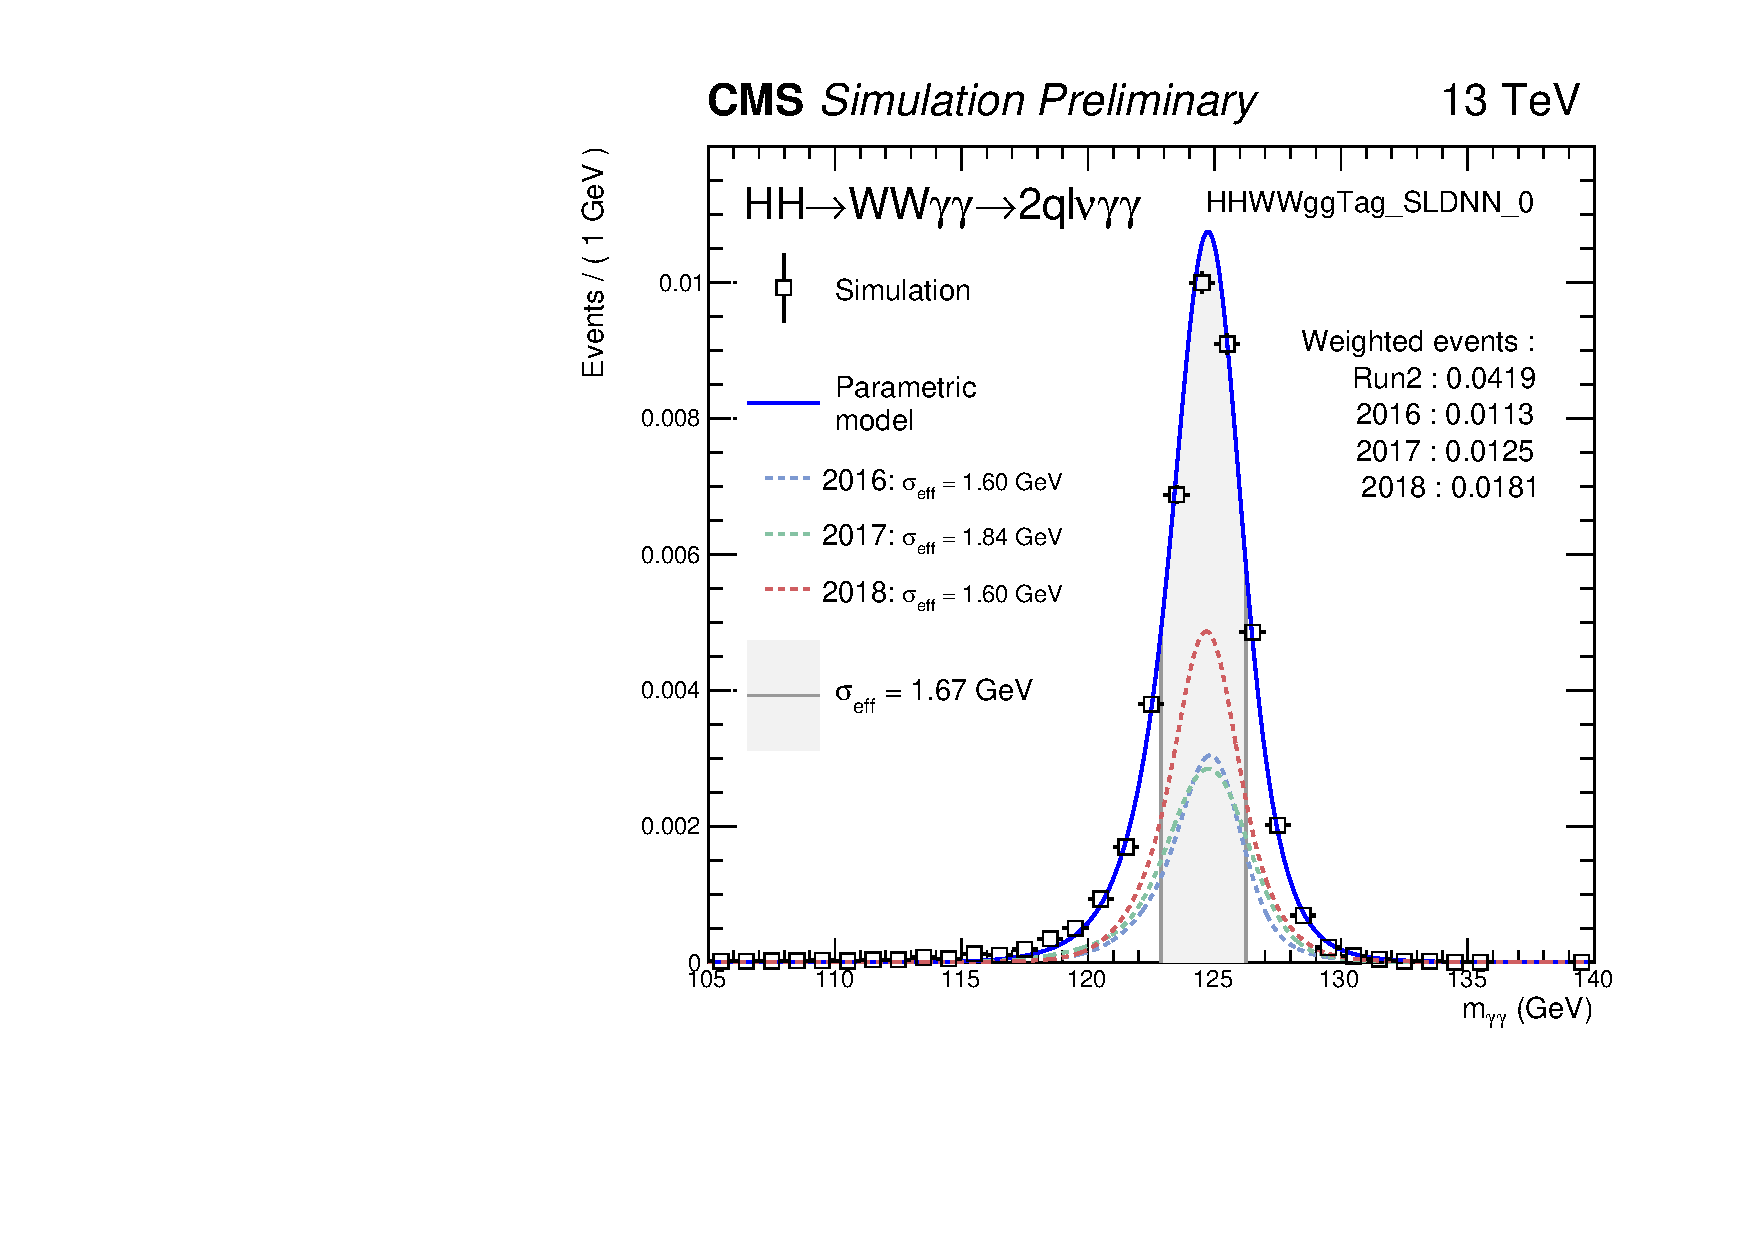
\includegraphics[width=0.45\textwidth]{Sections/HHWWgg/images/AnalyticFitting/Signal/smodel_HHWWggTag_SLDNN_0.pdf}}
    \qquad
    \subfloat[DNN Category 1]{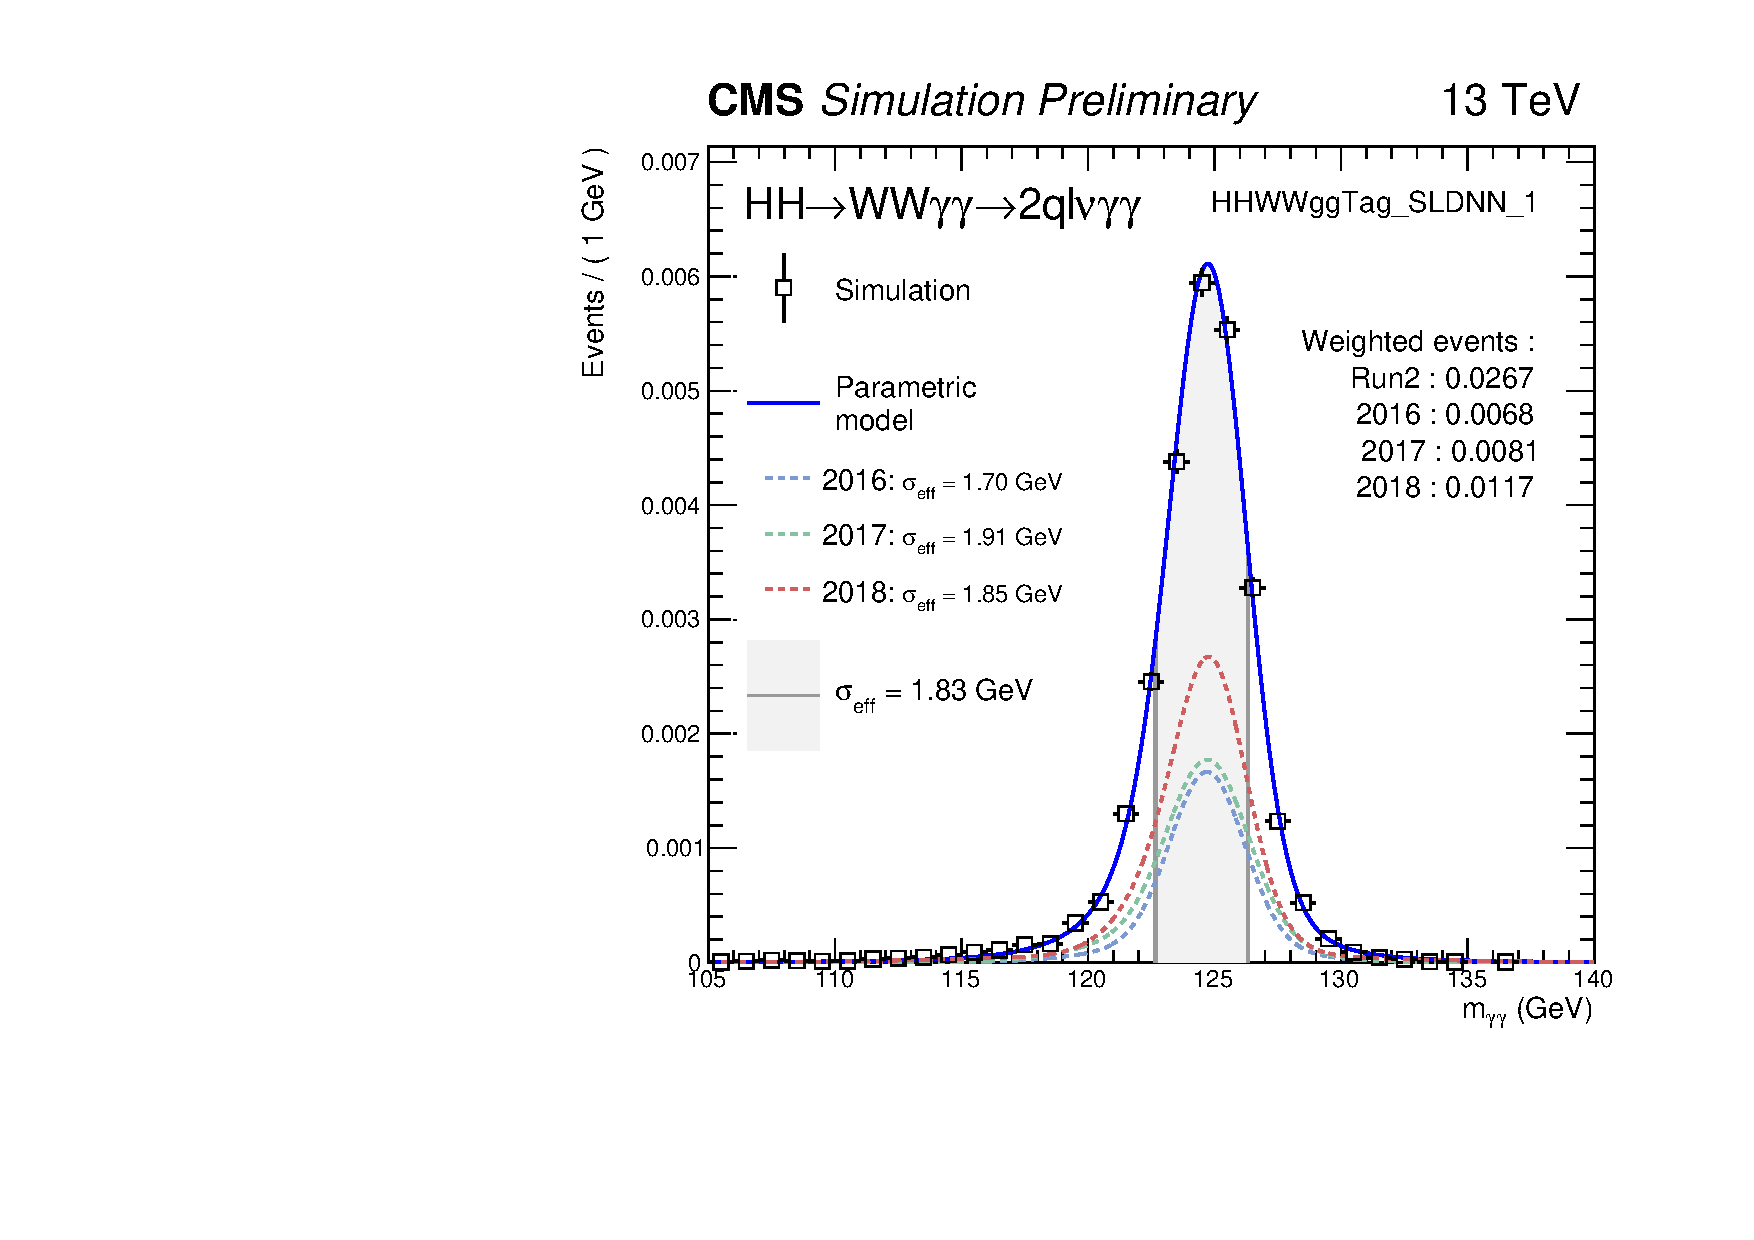
\includegraphics[width=0.45\textwidth]{Sections/HHWWgg/images/AnalyticFitting/Signal/smodel_HHWWggTag_SLDNN_1.pdf}}
    \caption{Semi-Leptonic signal models for all three years and the Run 2 combination, in the two highest DNN score categories.}
    \label{fig:SLSignal_01}
\end{figure}

For the Fully-Hadronic category, the remaining bb$\gamma\gamma$ and fully-hadronic ZZ$\gamma\gamma$ yields after the minimization of contamination in the WW$\gamma\gamma$ phase space are considered HH signal in this category when extracting upper limits the di-Higgs cross section. Signal
model fits are shown for the Fully-Hadronic WW, ZZ, and bb$\gamma\gamma$ categories in Figures \ref{fig:FHWWSignal}, \ref{fig:FHZZSignal}, and  \ref{fig:FHBBSignal} respectively. These signal models
are combined before fitting to data in the Fully-Hadronic categories.

\begin{figure}[!htbp]
    \setcounter{subfigure}{0}
    \centering
    \subfloat[WW$\gamma\gamma$ signal model \label{fig:FHWWSignal}]{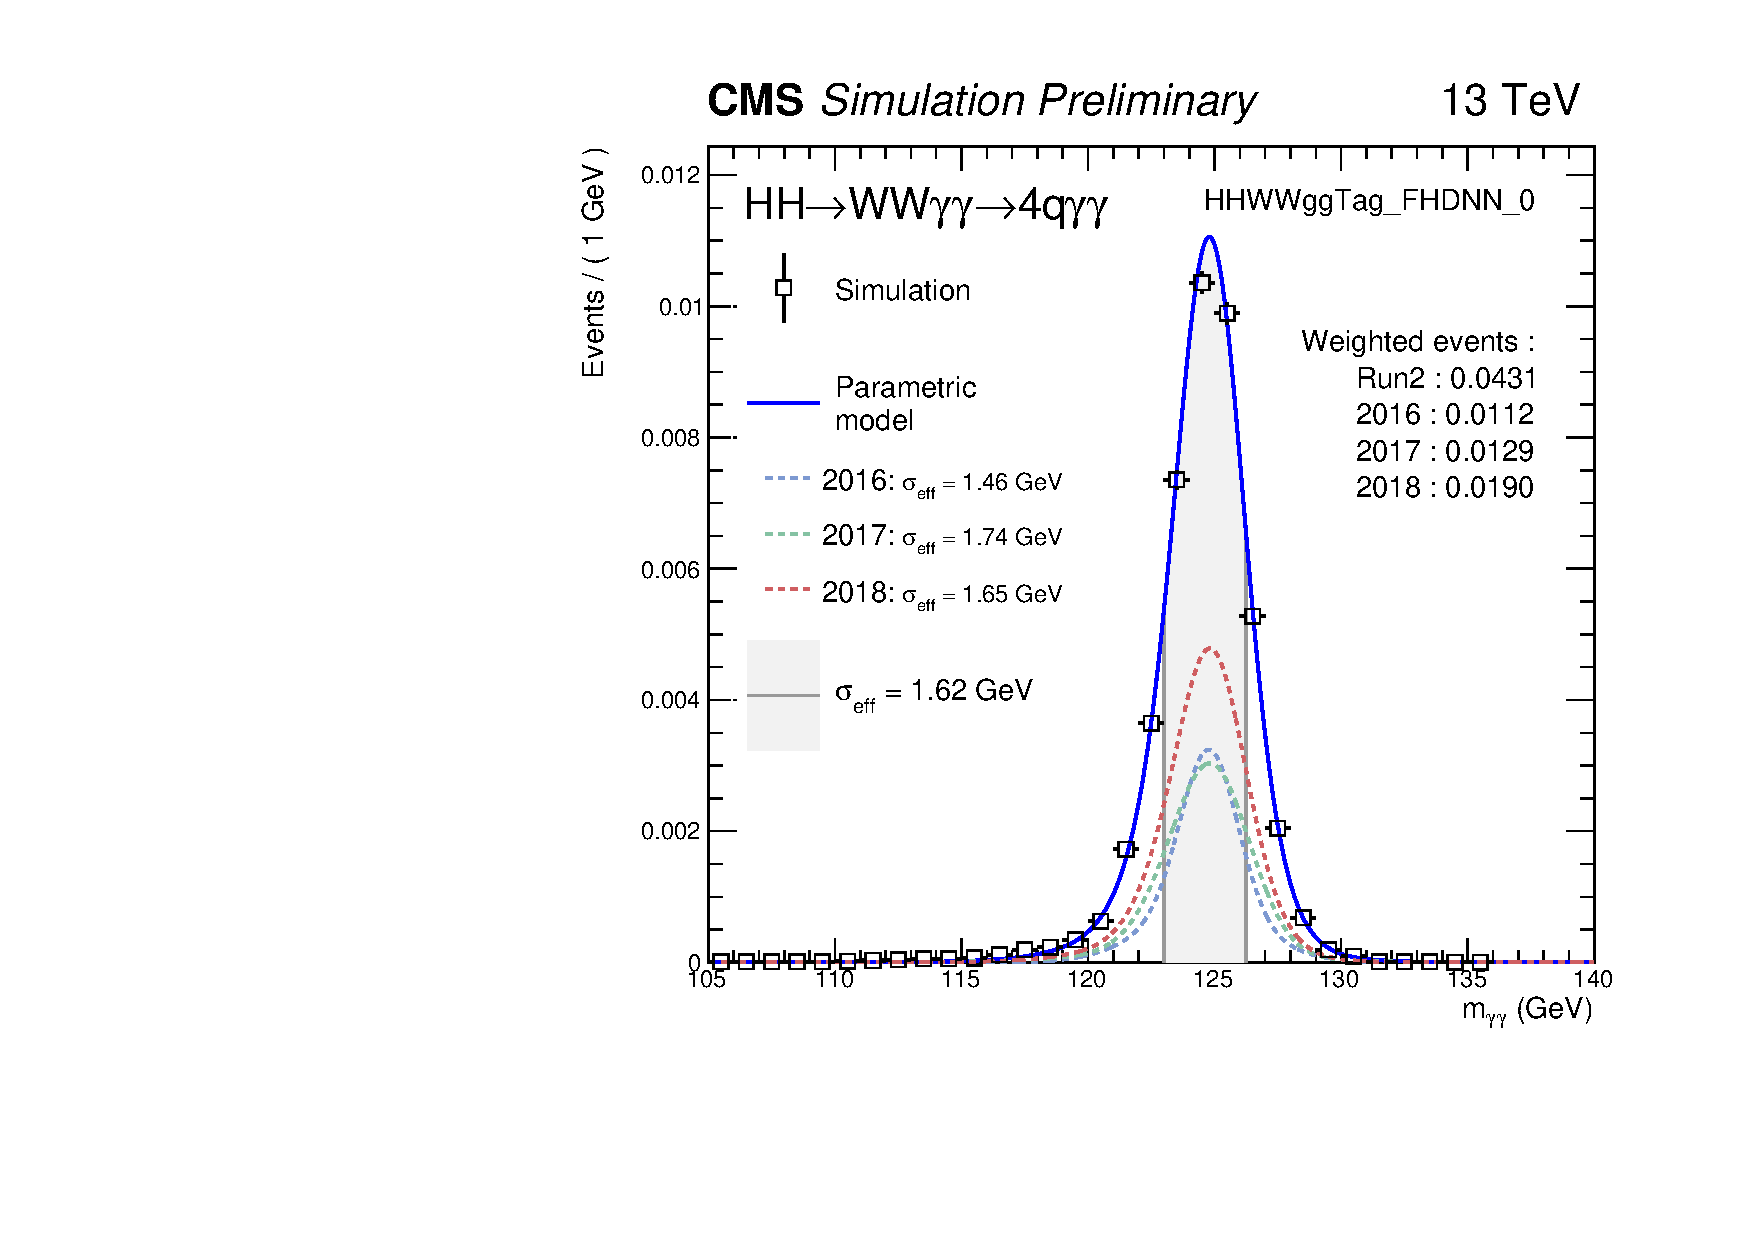
\includegraphics[width=0.45\textwidth]{Sections/HHWWgg/images/AnalyticFitting/Signal/FullyHadronic/smodel_HHWWggTag_FHDNN_0.pdf}}
    \qquad
    \subfloat[ZZ$\gamma\gamma$ signal model \label{fig:FHZZSignal}]{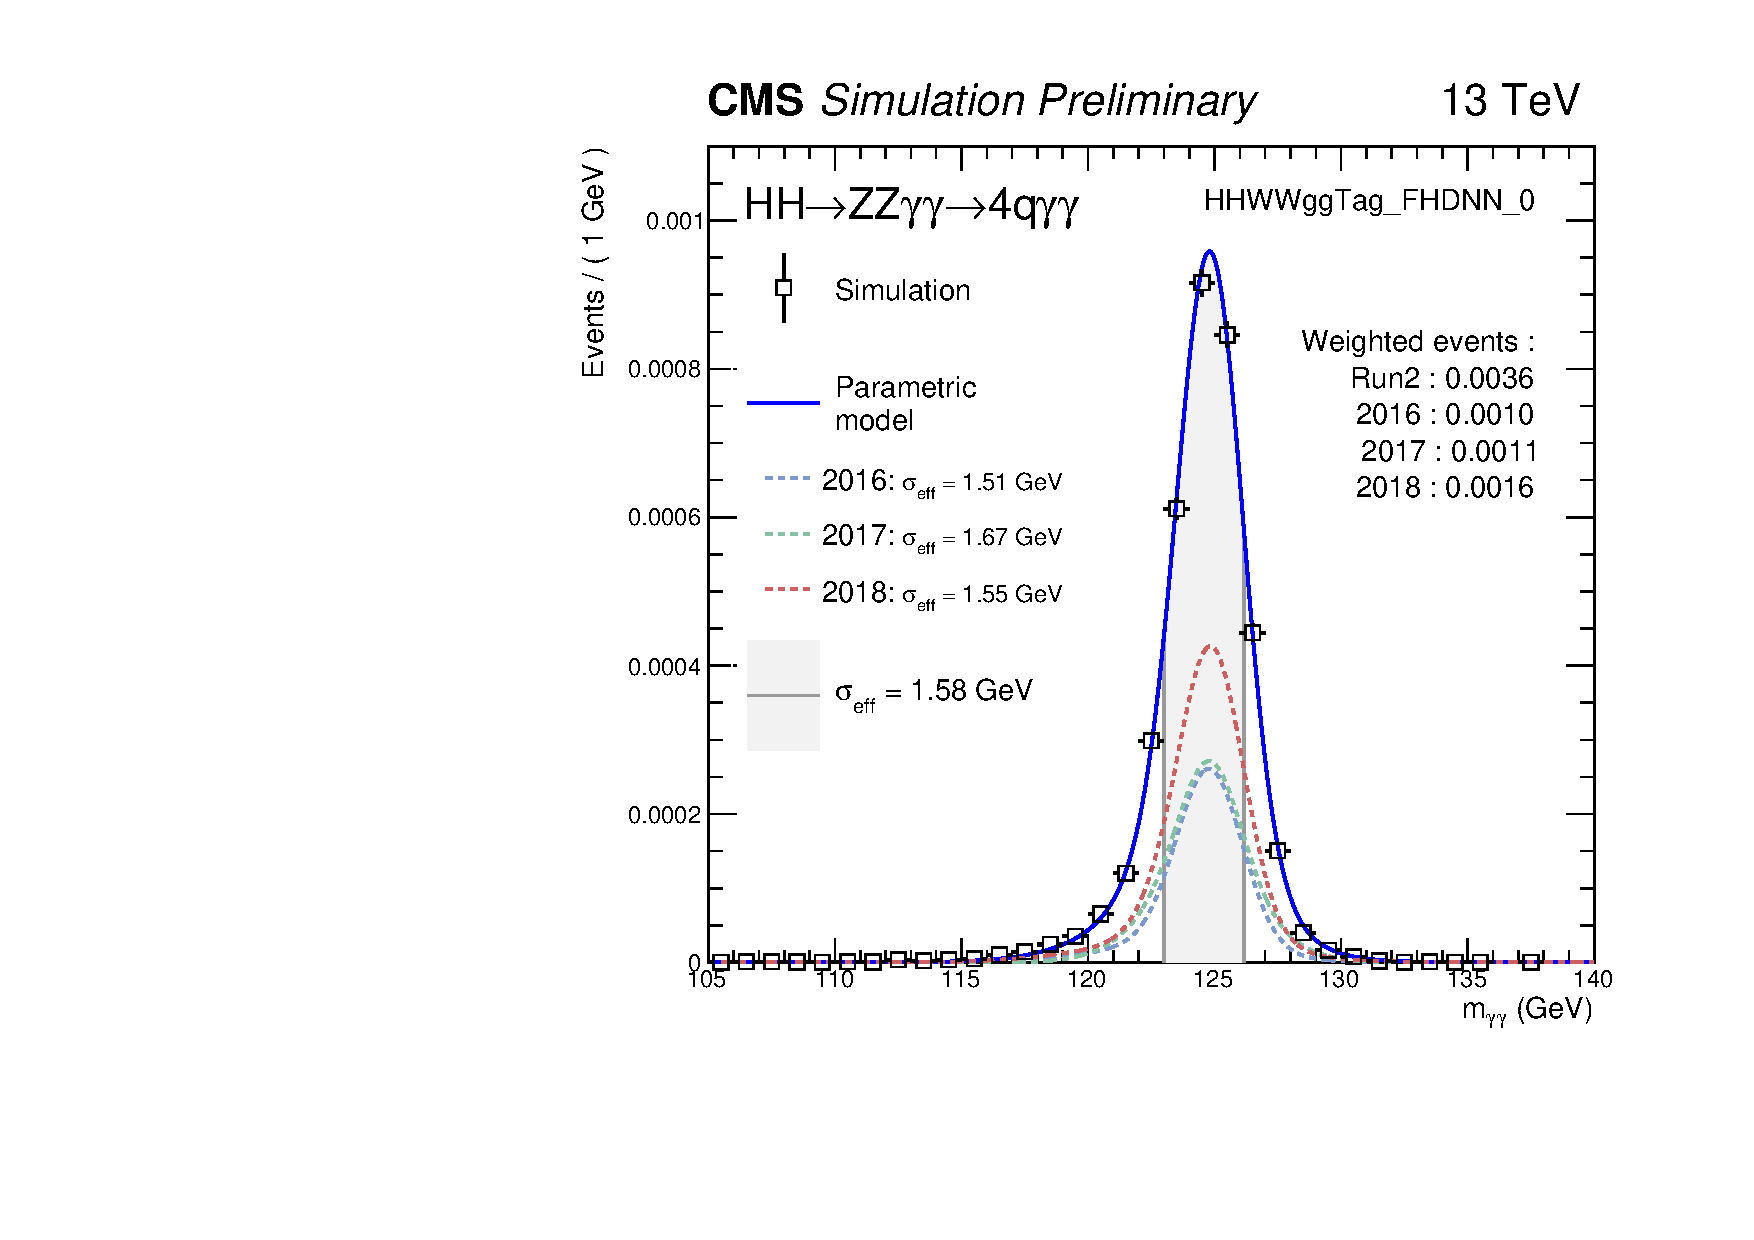
\includegraphics[width=0.45\textwidth]{Sections/HHWWgg/images/AnalyticFitting/Signal/FullyHadronic/smodel_HHZZggTag_FHDNN_0.pdf}}
    \caption{Fully-Hadronic HH models for all three years and the Run 2 combination in the highest DNN score Fully-hadronic category.}
\end{figure}

For the fully-leptonic final state, after applying the object and event selections described in Sections \ref{sec:Objects} and \ref{sec:FullyLeptonicEventSelections},
a signal fit model is produced using the remaining events. The signal model is shown in Figure \ref{fig:FLSignal}.

\begin{figure}[!htbp]
    \setcounter{subfigure}{0}
    \centering
    \subfloat[Fully-Hadronic bb$\gamma\gamma$ signal models for all three years and the Run 2 combination in the highest DNN score Fully-hadronic category. \label{fig:FHBBSignal}]{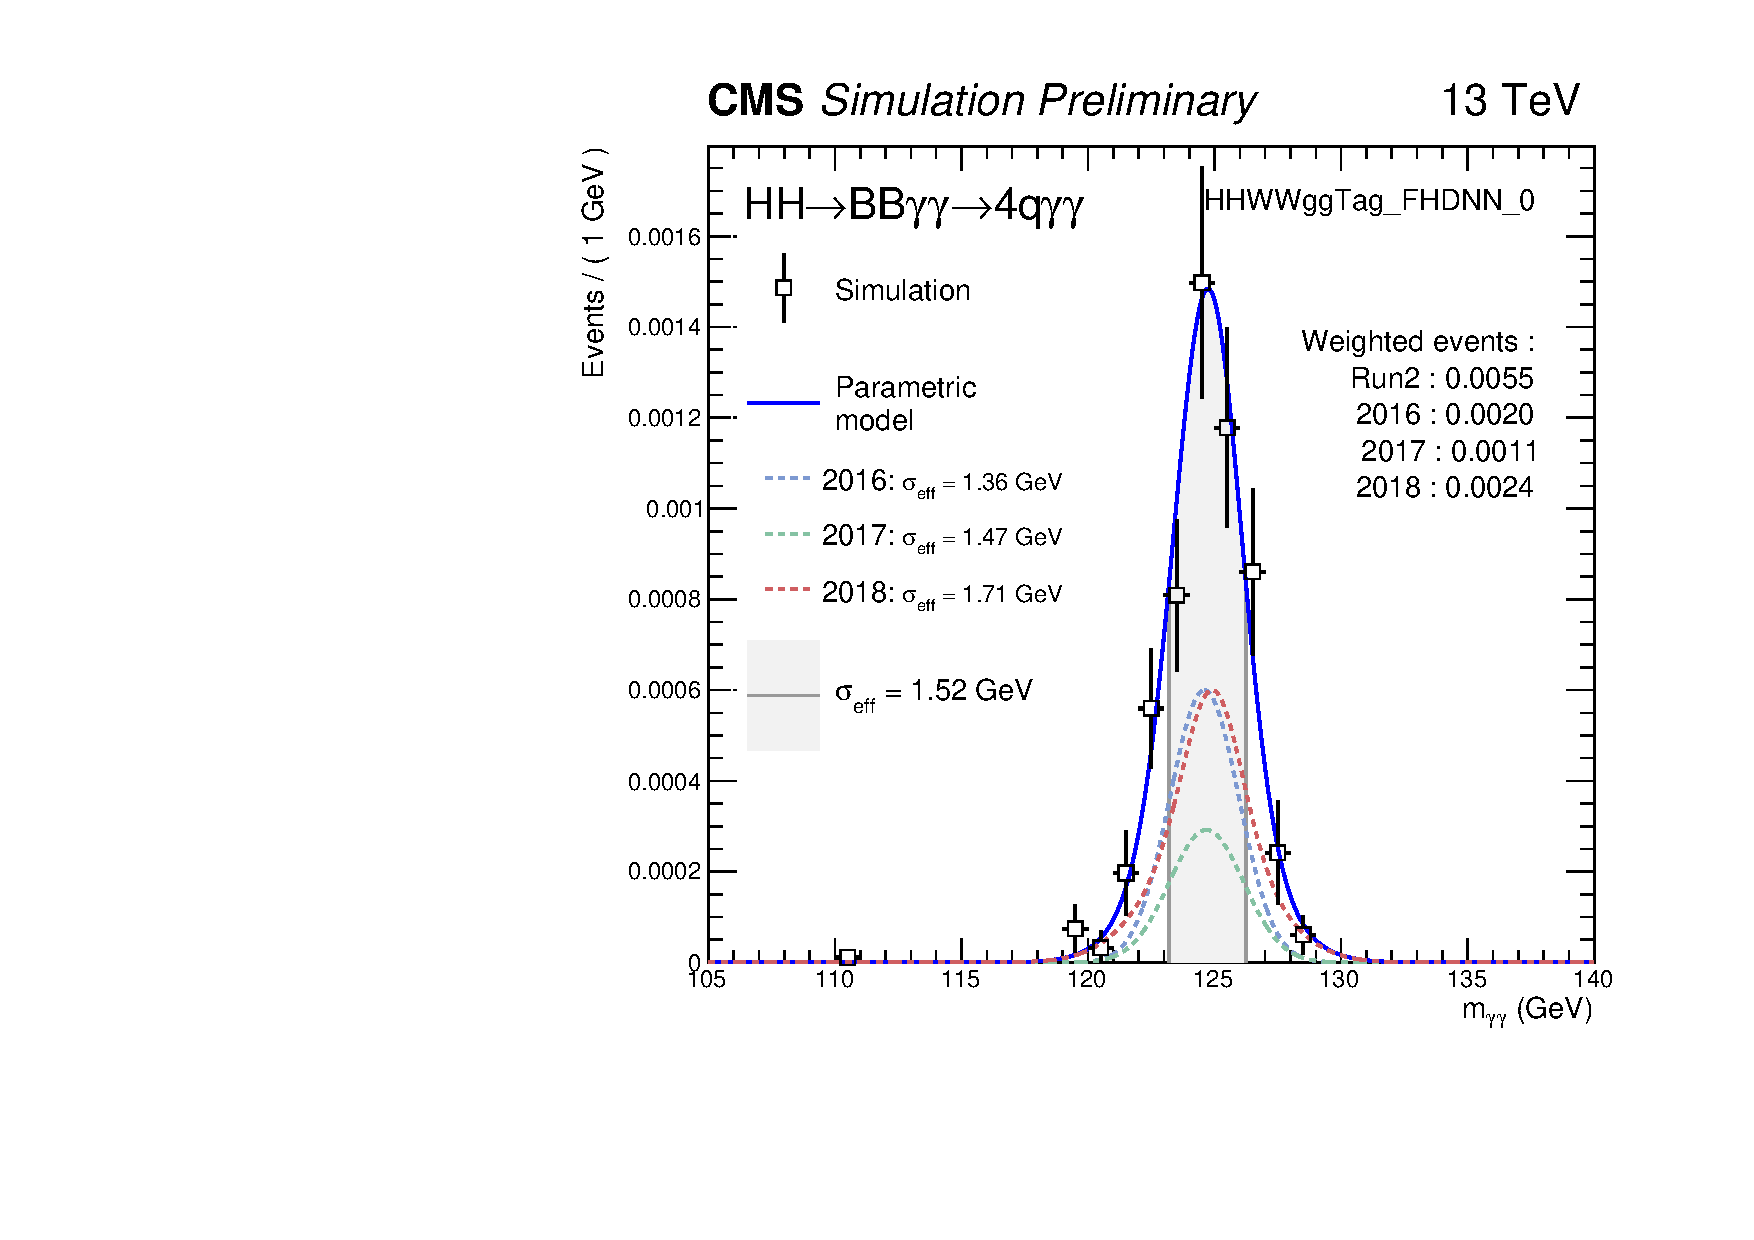
\includegraphics[width=0.45\textwidth]{Sections/HHWWgg/images/AnalyticFitting/Signal/FullyHadronic/smodel_HHBBggTag_FHDNN_0.pdf}}
    \qquad
    \subfloat[Fully-Leptonic signal models for all three years and the Run 2 combination \label{fig:FLSignal}]{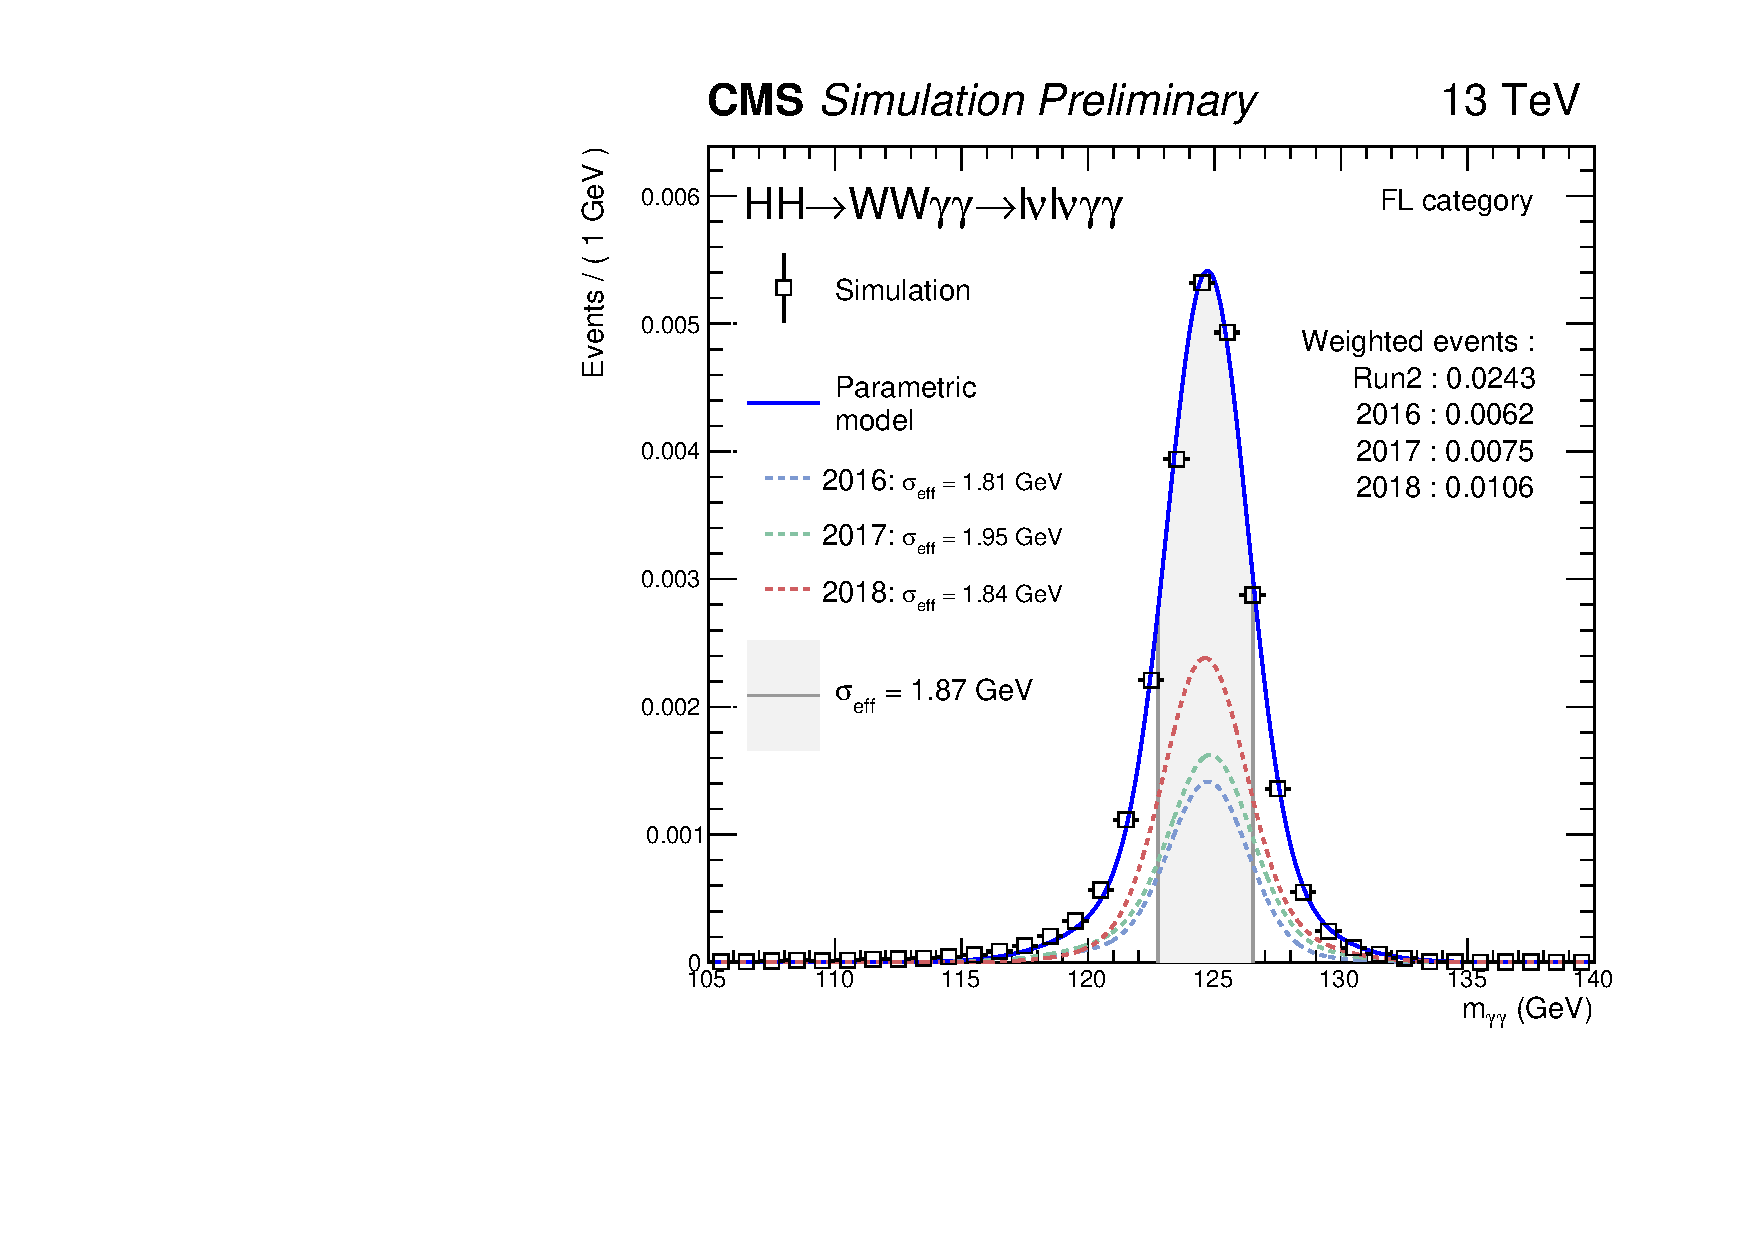
\includegraphics[width=0.45\textwidth]{Sections/HHWWgg/images/AnalyticFitting/Signal/smodel_all_FL.pdf}}
    \caption{Fully-Hadronic HH$\rightarrow$bb$\gamma\gamma$ and Fully-leptonic signal models for all three years and the Run 2 combination.}
\end{figure}

For all categories, the total number of signal events increases by year as expected due to the increase in integrated luminosity per year.

\clearpage
\subsection{Single Higgs Background}

There are expected resonant background processes present in the signal region, $115 < \mgg < 135$, due to $H\rightarrow\gamma\gamma$ processes, which cannot be modeled with a data-driven
method using data sideband events. These backgrounds are modeled with MC in the same fashion as the $HH\rightarrow WW\gamma\gamma$ signals in Section \ref{sec:SignalFitting}. Examples of some
Single Higgs models in the Semi-leptonic, Fully-hadronic and Fully-leptonic categories can
be seen in Figures \ref{fig:SL_SingleHiggs}, \ref{fig:FH_SingleHiggs}, and \ref{fig:FL_SingleHiggs}. Note that the ggH and VBFH single higgs signals are not provided for the Fully-Leptonic final state, as their contributions are either zero due to the absence of any
signal events passing the Fully-Leptonic selections, or are extremely low and can not be reasonably fit to an analytic model.

\begin{figure}[h!]
    \setcounter{subfigure}{0}
    \centering
    \subfloat[VHToGG]{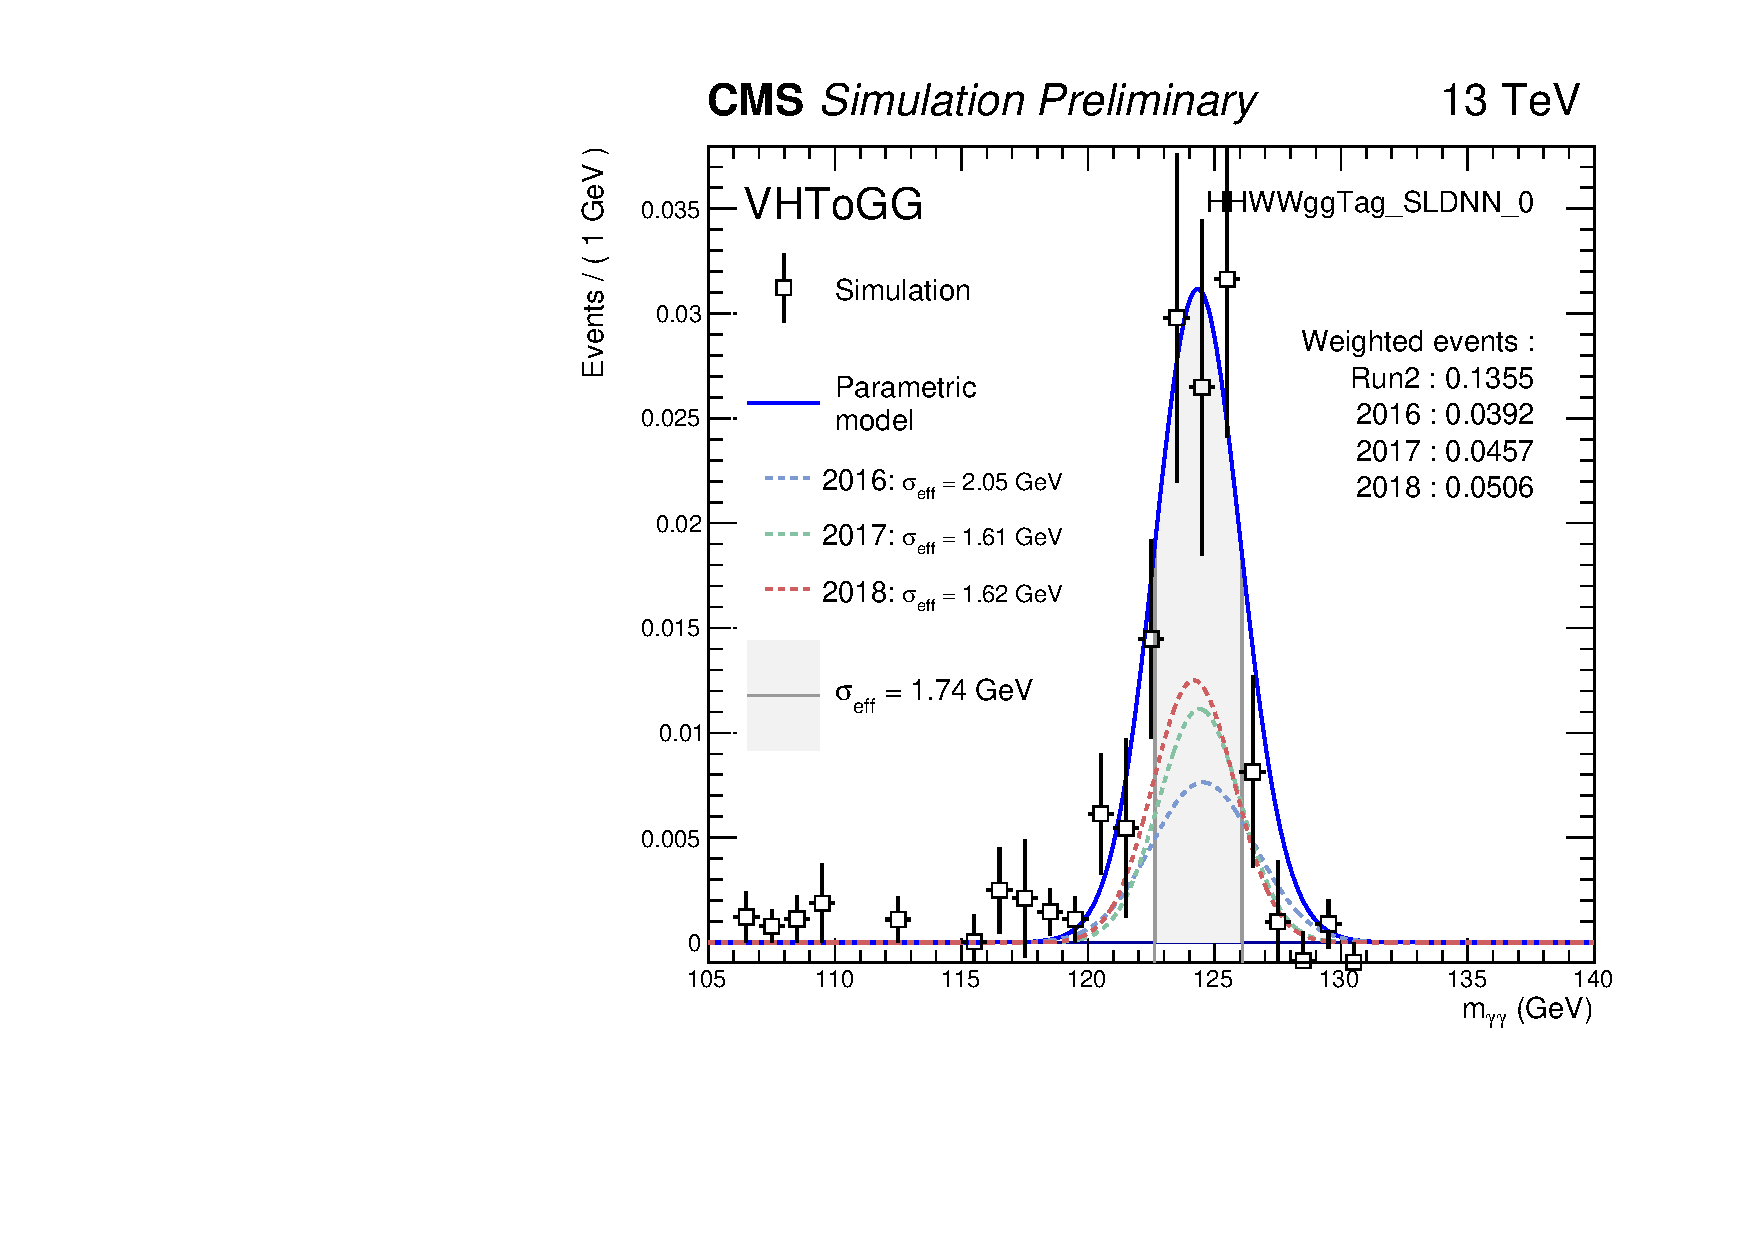
\includegraphics[width=0.45\textwidth]{Sections/HHWWgg/images/AnalyticFitting/SingleHiggs/VH/SL/smodel_HHWWggTag_SLDNN_0.pdf}}
    \qquad
    \subfloat[ttHJetToGG]{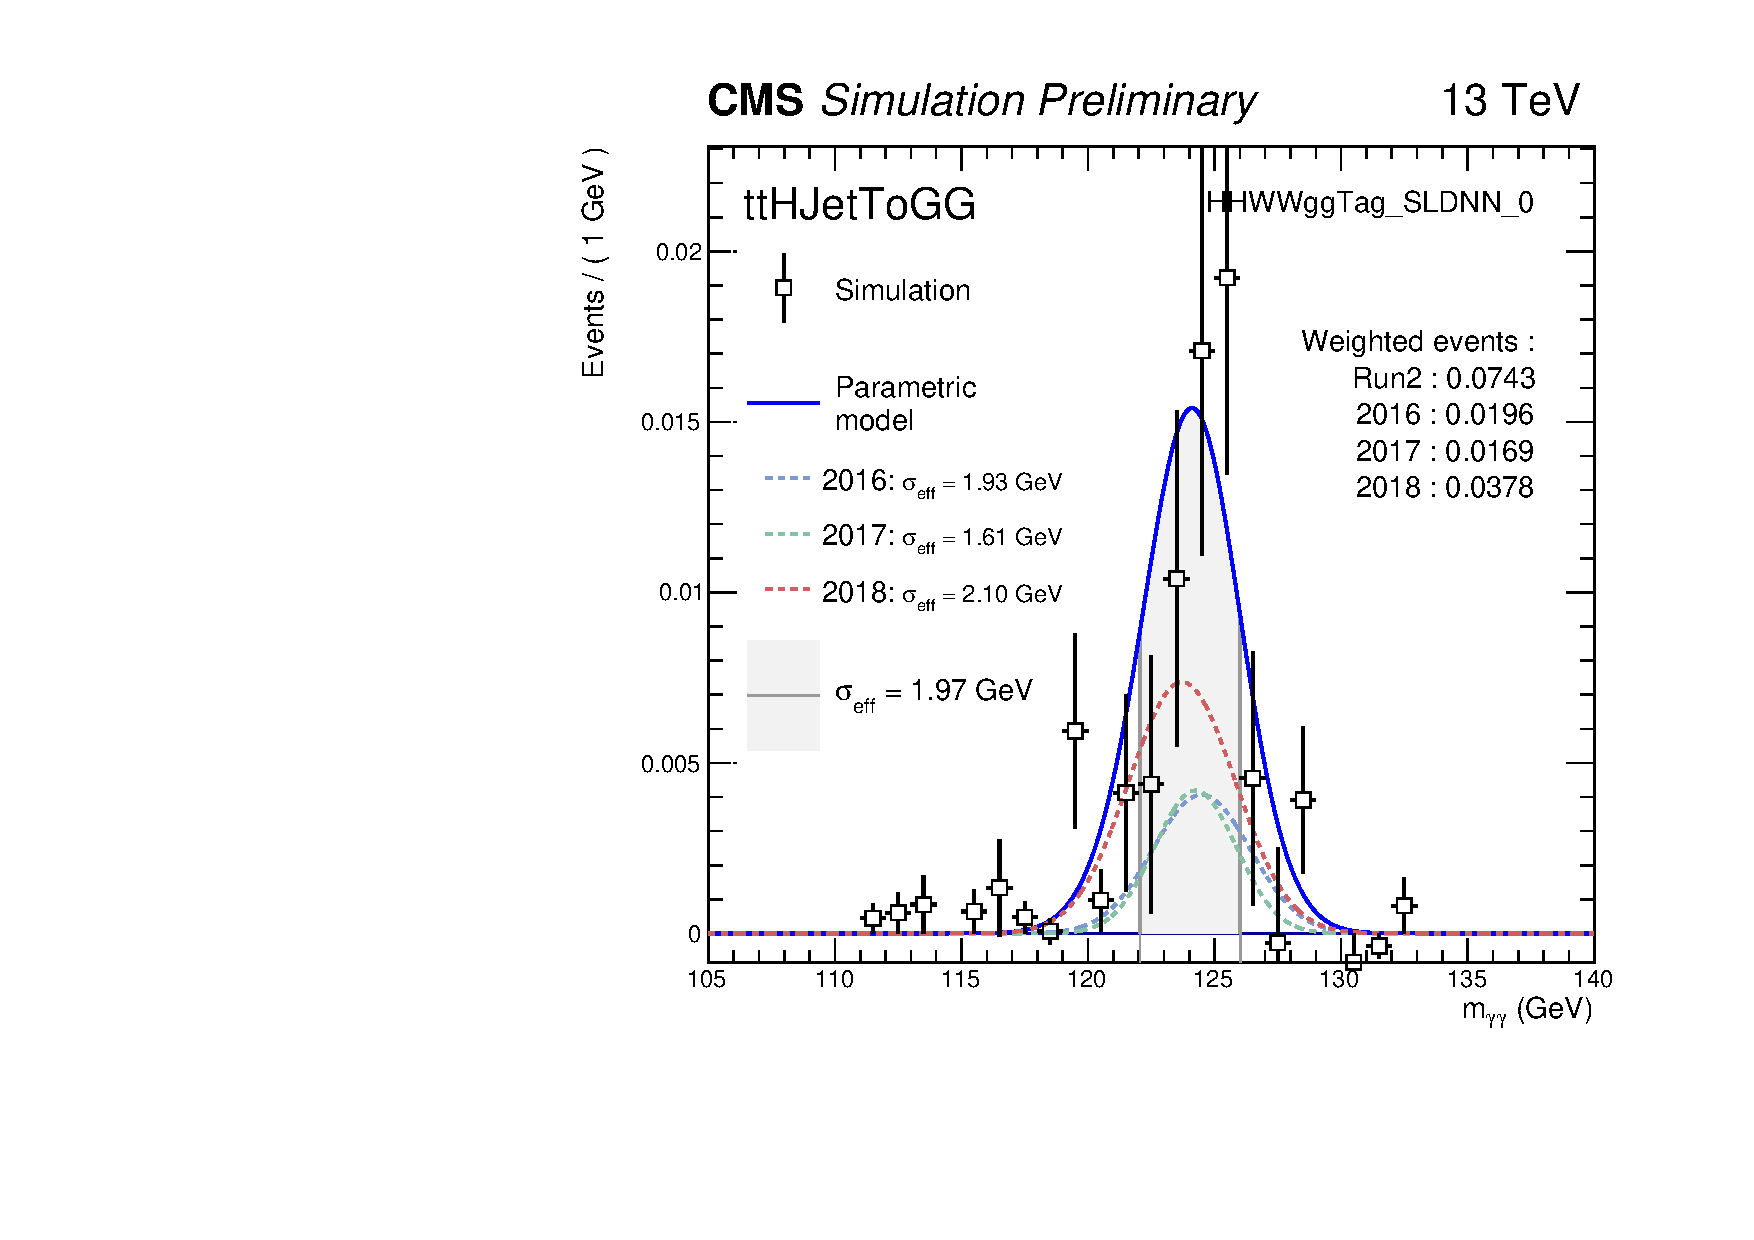
\includegraphics[width=0.45\textwidth]{Sections/HHWWgg/images/AnalyticFitting/SingleHiggs/ttHJet/SL/smodel_HHWWggTag_SLDNN_0.pdf}}
    \caption{Semi-Leptonic DNN Category 0 Single Higgs Models}
    \label{fig:SL_SingleHiggs}
\end{figure}

\begin{figure}[!htbp]
    \setcounter{subfigure}{0}
    \centering
    \subfloat[ggH\label{fig:FH_SingleHiggs_1}]{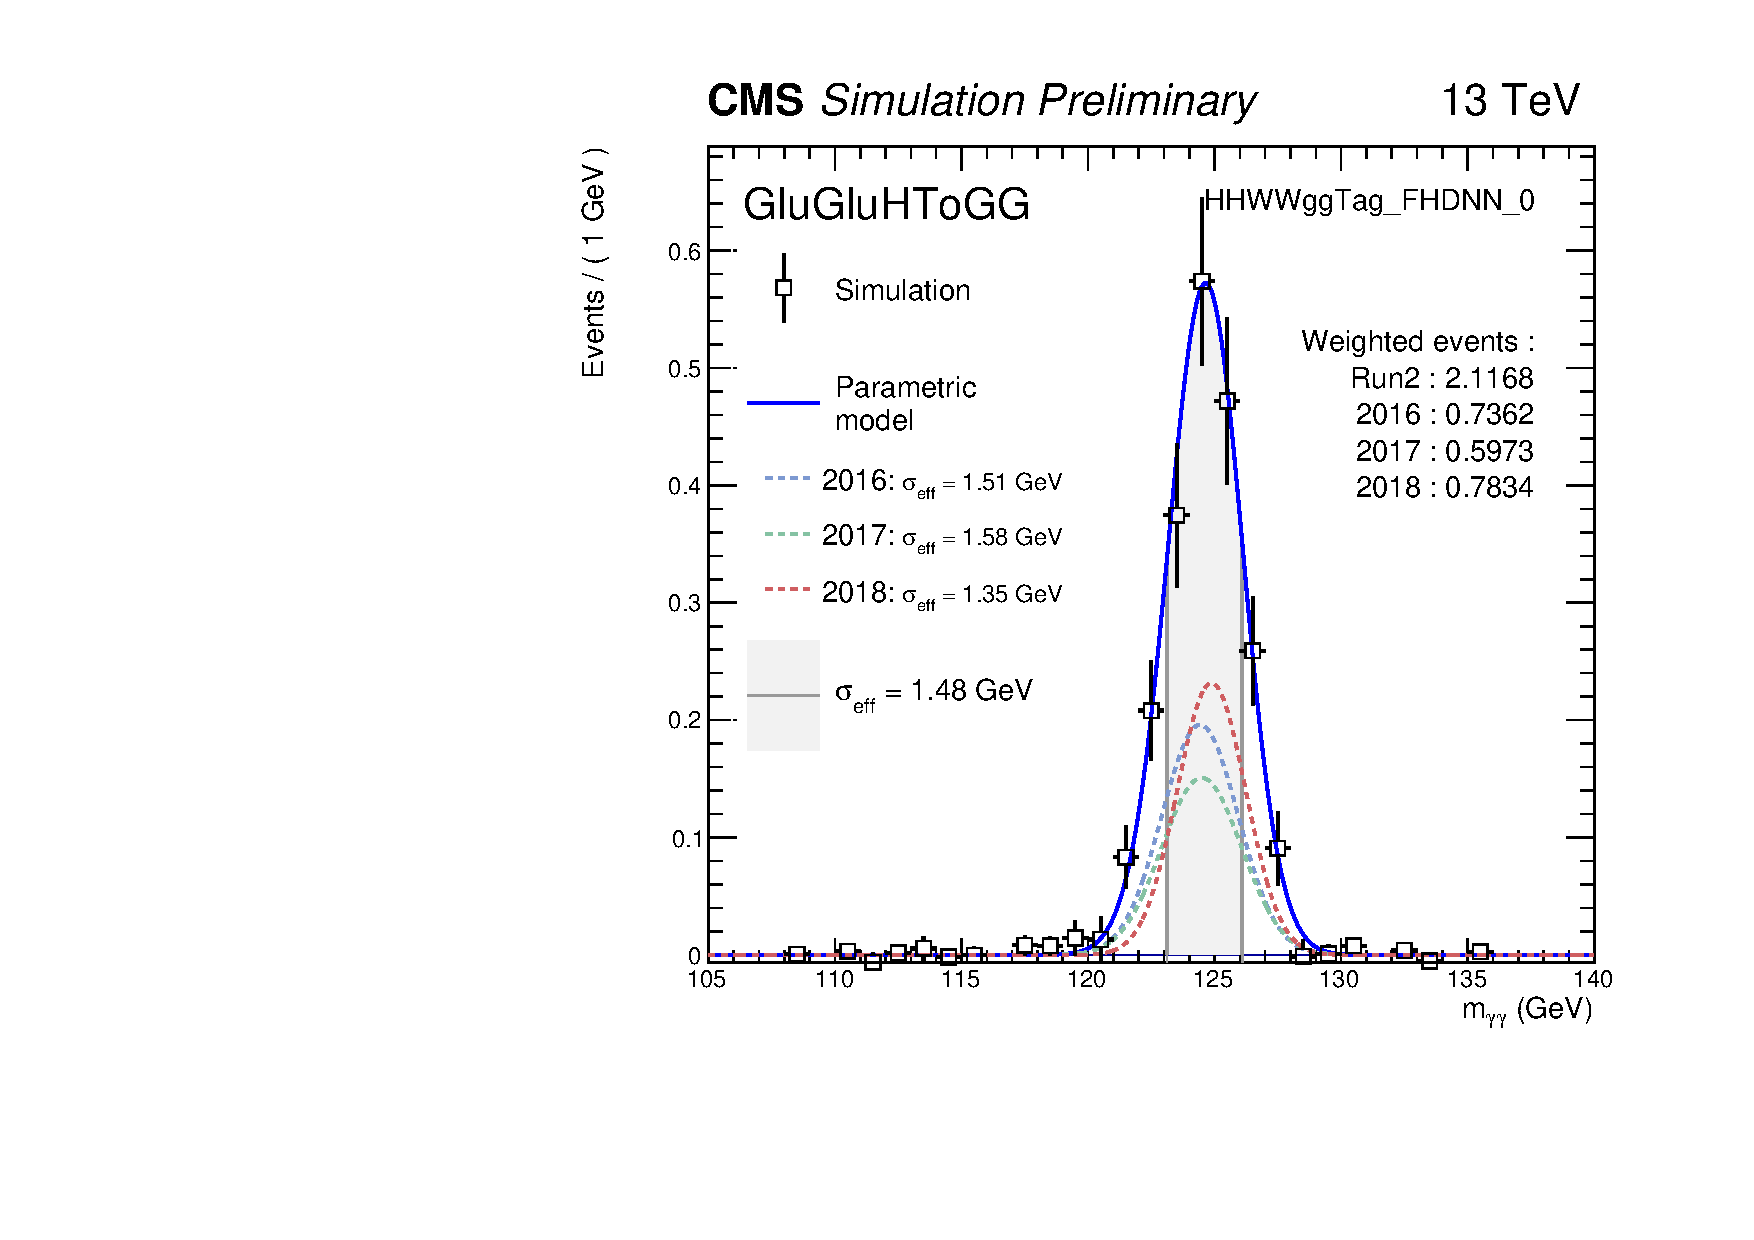
\includegraphics[width=0.45\textwidth]{Sections/HHWWgg/images/AnalyticFitting/SingleHiggs/ggH/FH/smodel_HHWWggTag_FHDNN_0.pdf}}
    \qquad
    \subfloat[VBFH\label{fig:FH_SingleHiggs_2}]{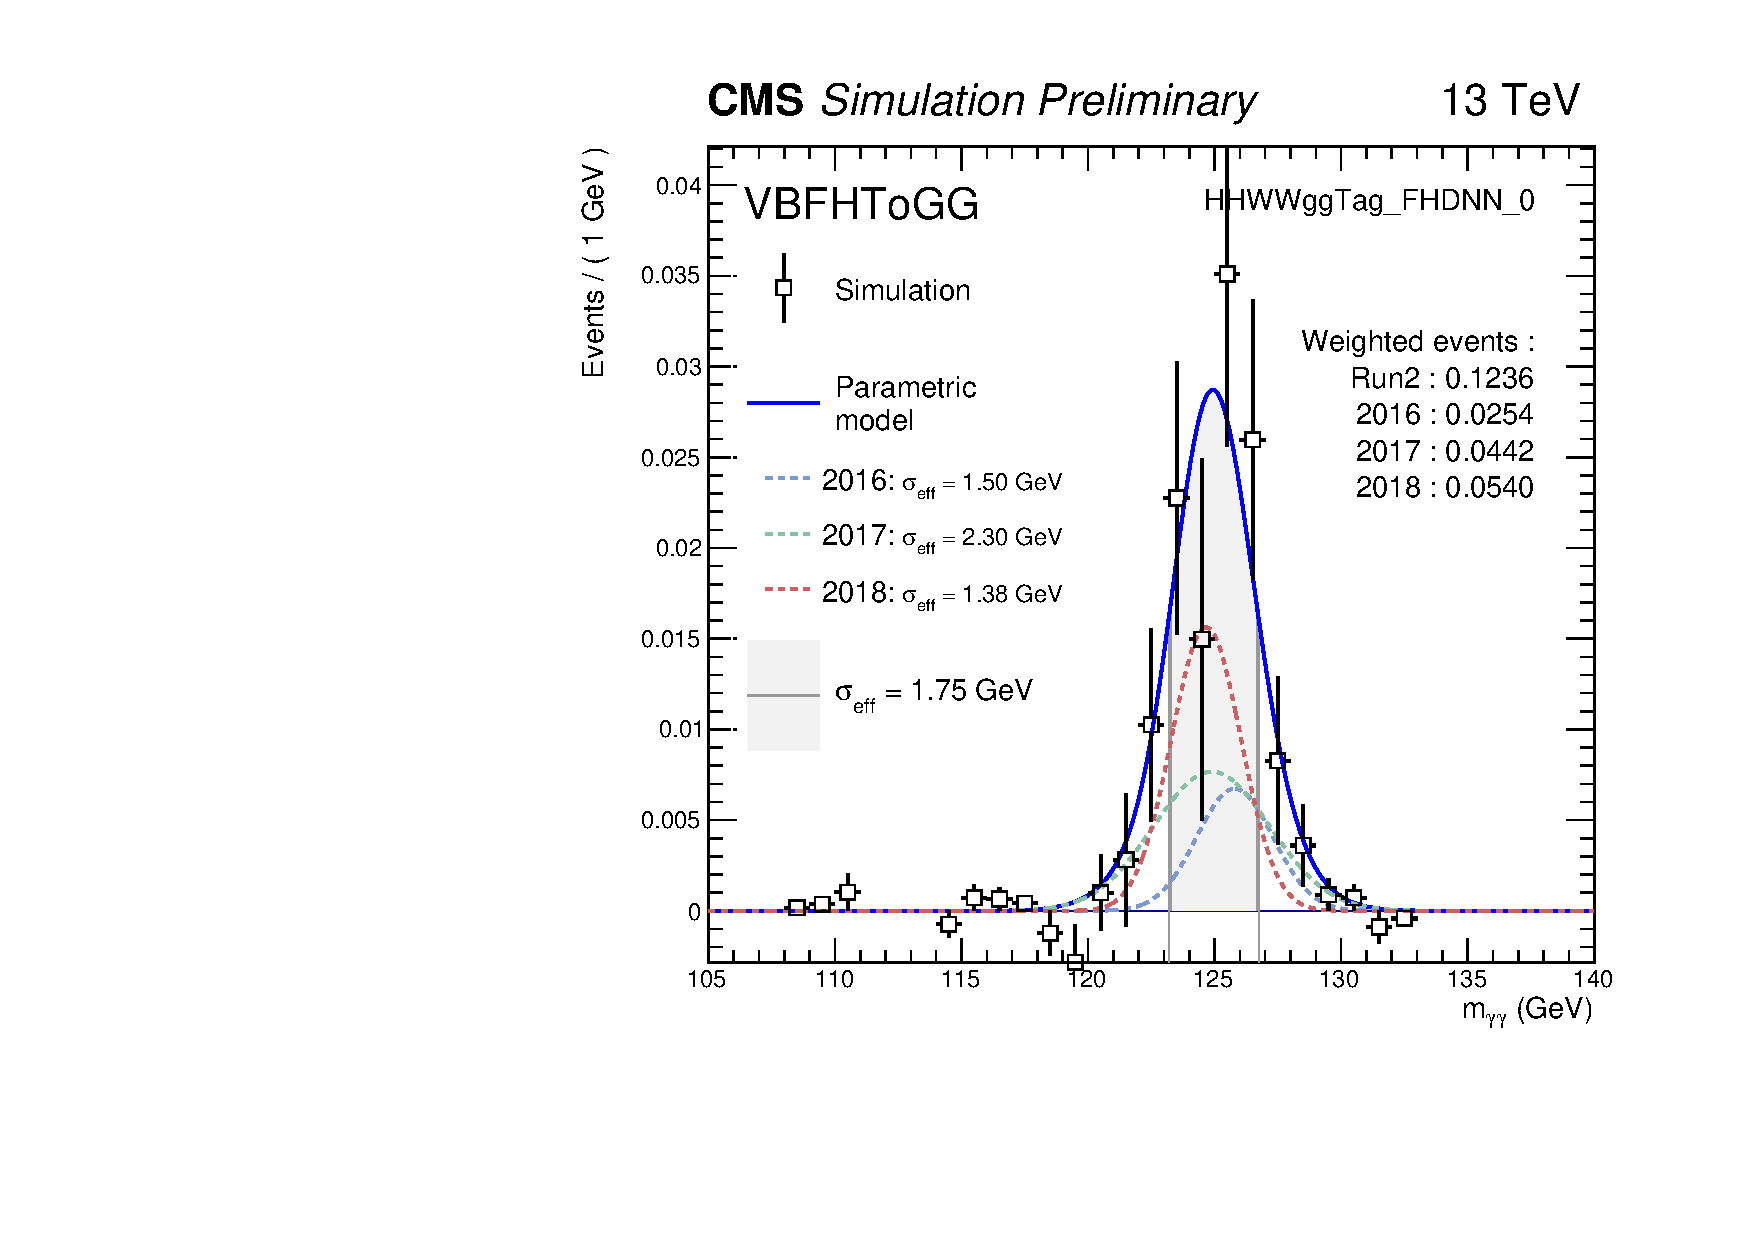
\includegraphics[width=0.45\textwidth]{Sections/HHWWgg/images/AnalyticFitting/SingleHiggs/VBFH/FH/smodel_HHWWggTag_FHDNN_0.pdf}}
    \caption{Fully-Hadronic single higgs models in the highest DNN score category.}
    \label{fig:FH_SingleHiggs}
\end{figure}

\begin{figure}[!htbp]
    \setcounter{subfigure}{0}
    \centering
    \subfloat[VHToGG]{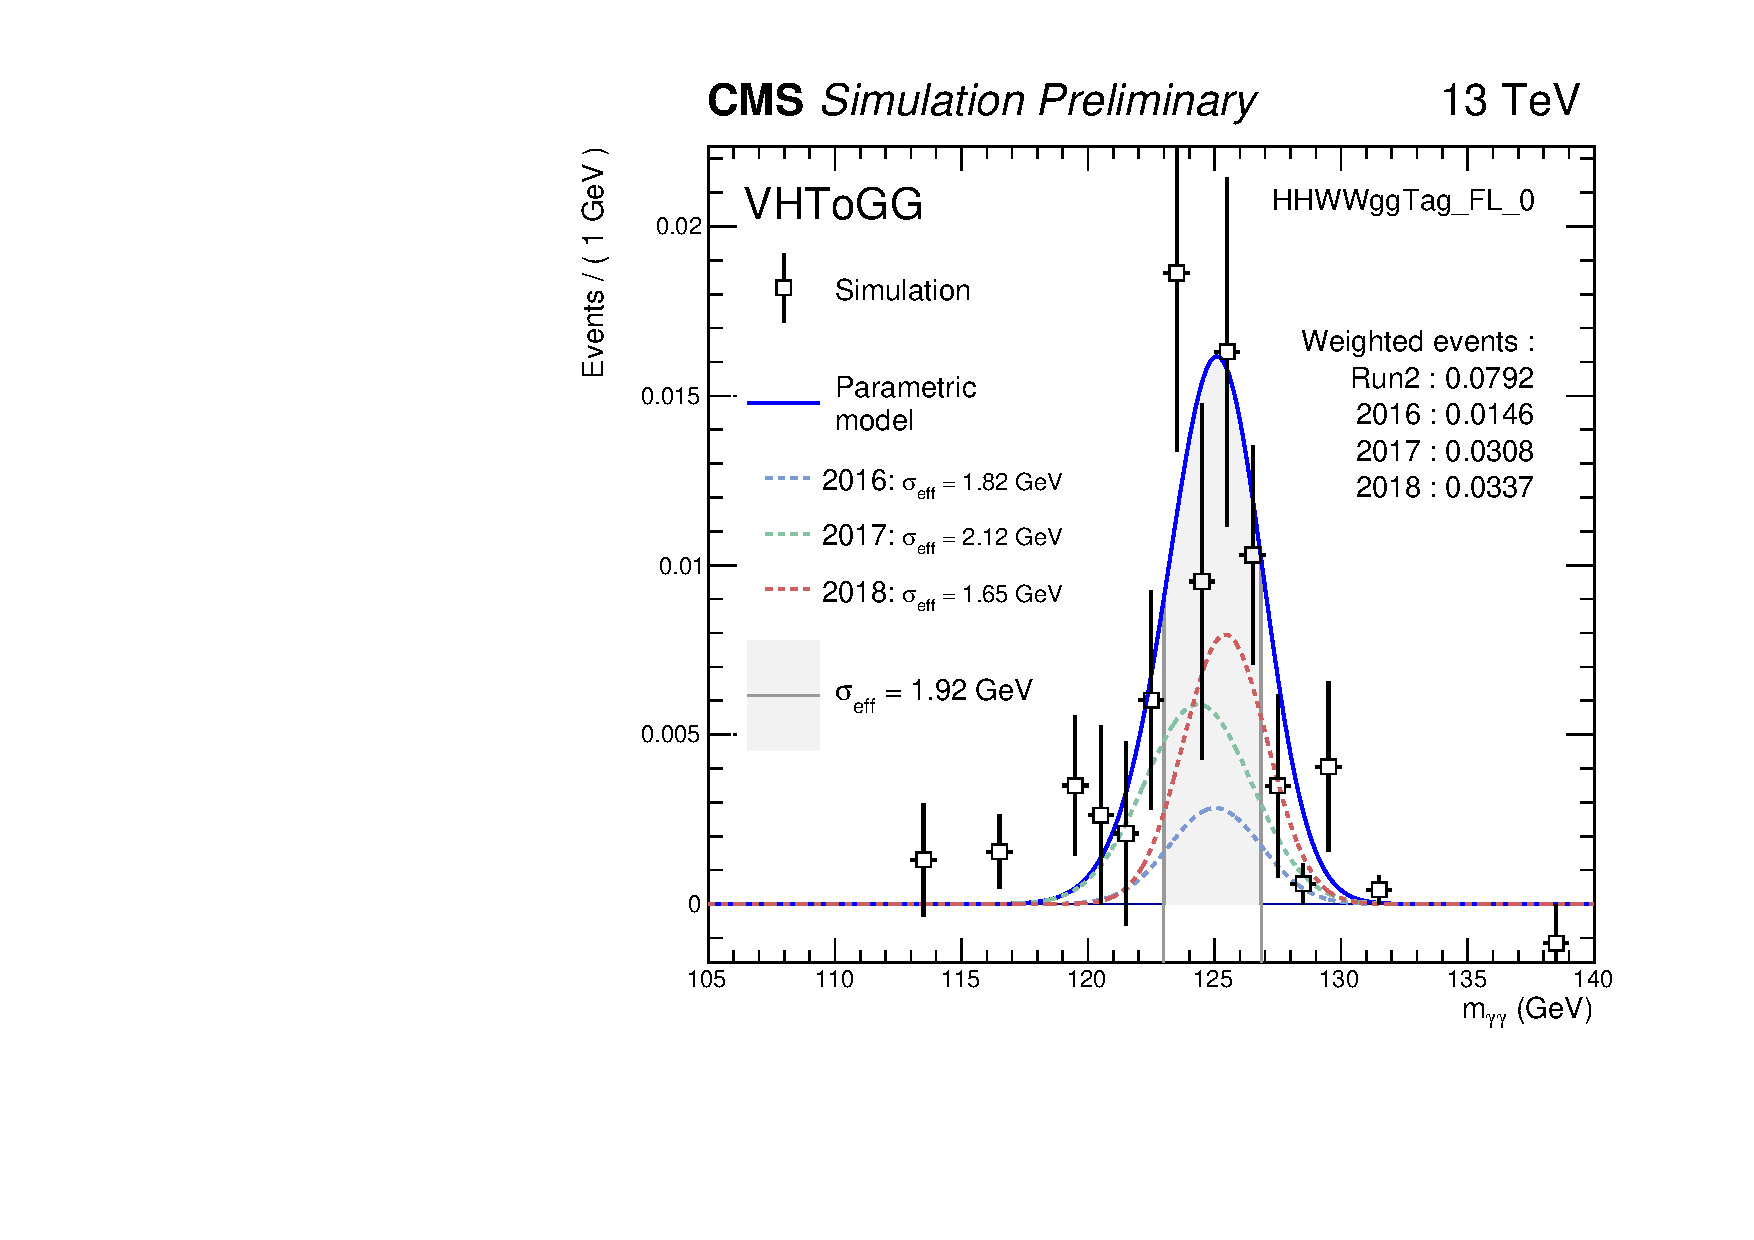
\includegraphics[width=0.45\textwidth]{Sections/HHWWgg/images/AnalyticFitting/SingleHiggs/VH/FL/smodel_all.pdf}}
    \qquad
    \subfloat[ttHJetToGG]{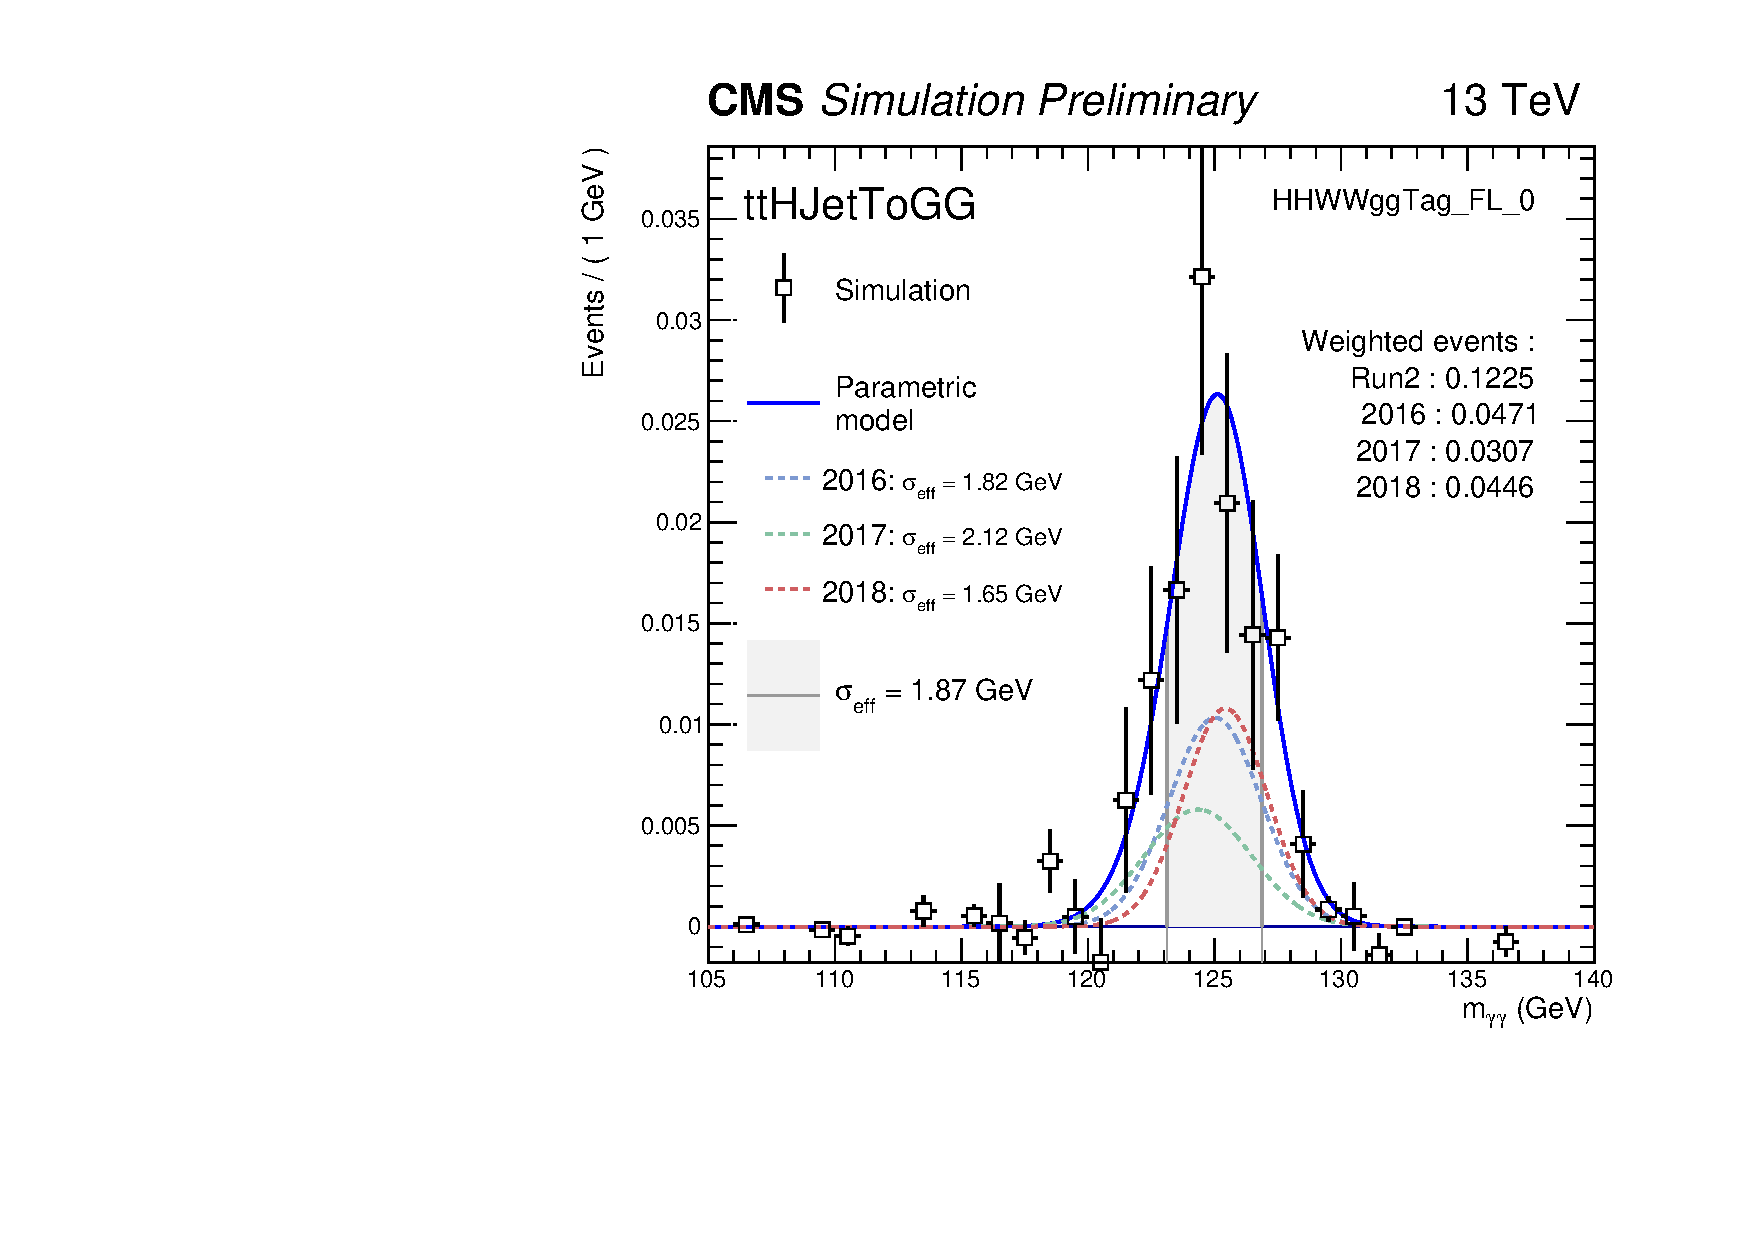
\includegraphics[width=0.45\textwidth]{Sections/HHWWgg/images/AnalyticFitting/SingleHiggs/ttHJet/FL/smodel_all.pdf}}
    \caption{Fully-Leptonic Single Higgs Models}
    \label{fig:FL_SingleHiggs}
\end{figure}

\clearpage

\subsection{Continuum Background}
\label{sec:AnalyticFitting_Background}

A data-driven background model is produced for each category using the data sidebands: events in the regions $100 < \mgg < 115$ and $135 < \mgg < 180$. The aim of this
is to model the continuum background. After the selections and categorizations of each final state category are applied to the 2016, 2017, and 2018 datasets, analytic functions are fit
to the resulting $m_{\gamma\gamma}$ distributions in the data sidebands for each analysis category. These are later combined with their corresponding single Higgs models in order to obtain a full background model. As
with the signal fitting, an F-Test is performed first in order to determine the most appropriate analytic function to fit to the data sidebands. Bernstein, laurent, exponential, and powerlaw function families are considered as
candidates to fit the data. The fit is then performed with the fit function shape determined from the F-Test.
In the Semi-Leptonic background fitting, the three data taking years are merged together before ftest and fitting are performed.
The ftests and S $+$ B fits for the Semi-Leptonic channel, where the HH signal model is scaled to the resulting simultaneous best fit to data in all WW$\gamma\gamma$ categories, are shown in Figures \ref{fig:SL_DataDrivenbkg_Run2_SLDNN_0}, \ref{fig:SL_DataDrivenbkg_Run2_SLDNN_1},
\ref{fig:SL_DataDrivenbkg_Run2_SLDNN_2} and \ref{fig:SL_DataDrivenbkg_Run2_SLDNN_3}. The f-tests and fits for the Fully-Hadronic
category is shown in Figures \ref{fig:FH_SidebandFits}. For the Fully-Leptonic category only, due to a low number of sideband events per year,
a single full Run2 continuum background model is produced by summing the three years of sideband data before performing an f-Test and producing a fit model, where uncertainty is obtained via the envelope method, which can be seen in Figure \ref{fig:FL_DataDrivenbkg_Run2}.
A best fit function is chosen by treating the choice of function as a discrete nuisance parameter.
An uncertainty is then assigned to the chosen fit function based on a combination of the likelihoods of all attempted fit functions. This method is described in
Ref. \cite{Dauncey_2015}. Note that in the lower panel plots for all data-driven background fit plots, the quantity shown is the data with the single Higgs and continuum background components subtracted. 
% \newpage
\begin{figure}[!htbp]
    \setcounter{subfigure}{0}
    \centering
    \subfloat[fTest]{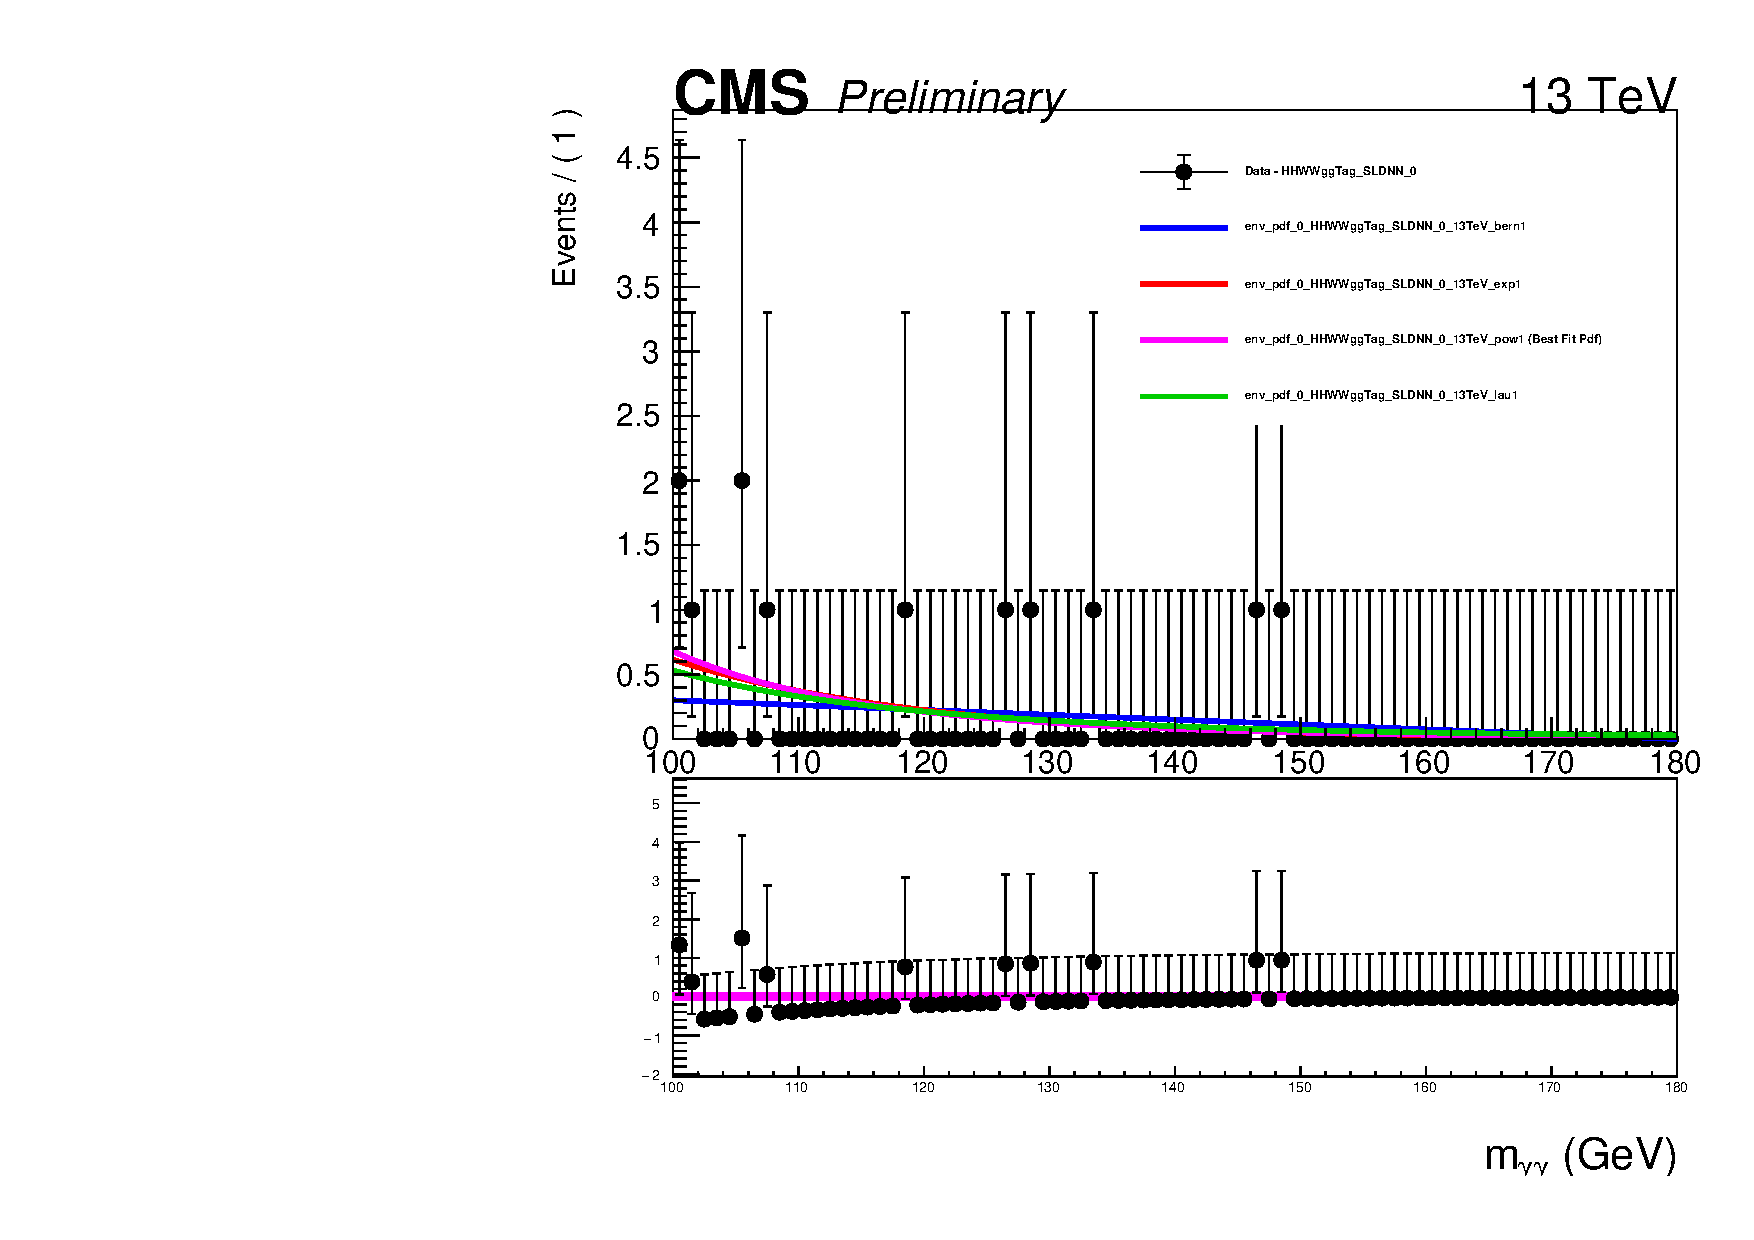
\includegraphics[width=0.45\textwidth]{Sections/HHWWgg/images/AnalyticFitting/ContinuumBackground/SL/Run2/multipdf_HHWWggTag_SLDNN_0.pdf}}
    \qquad
    \subfloat[Fit with uncertainty]{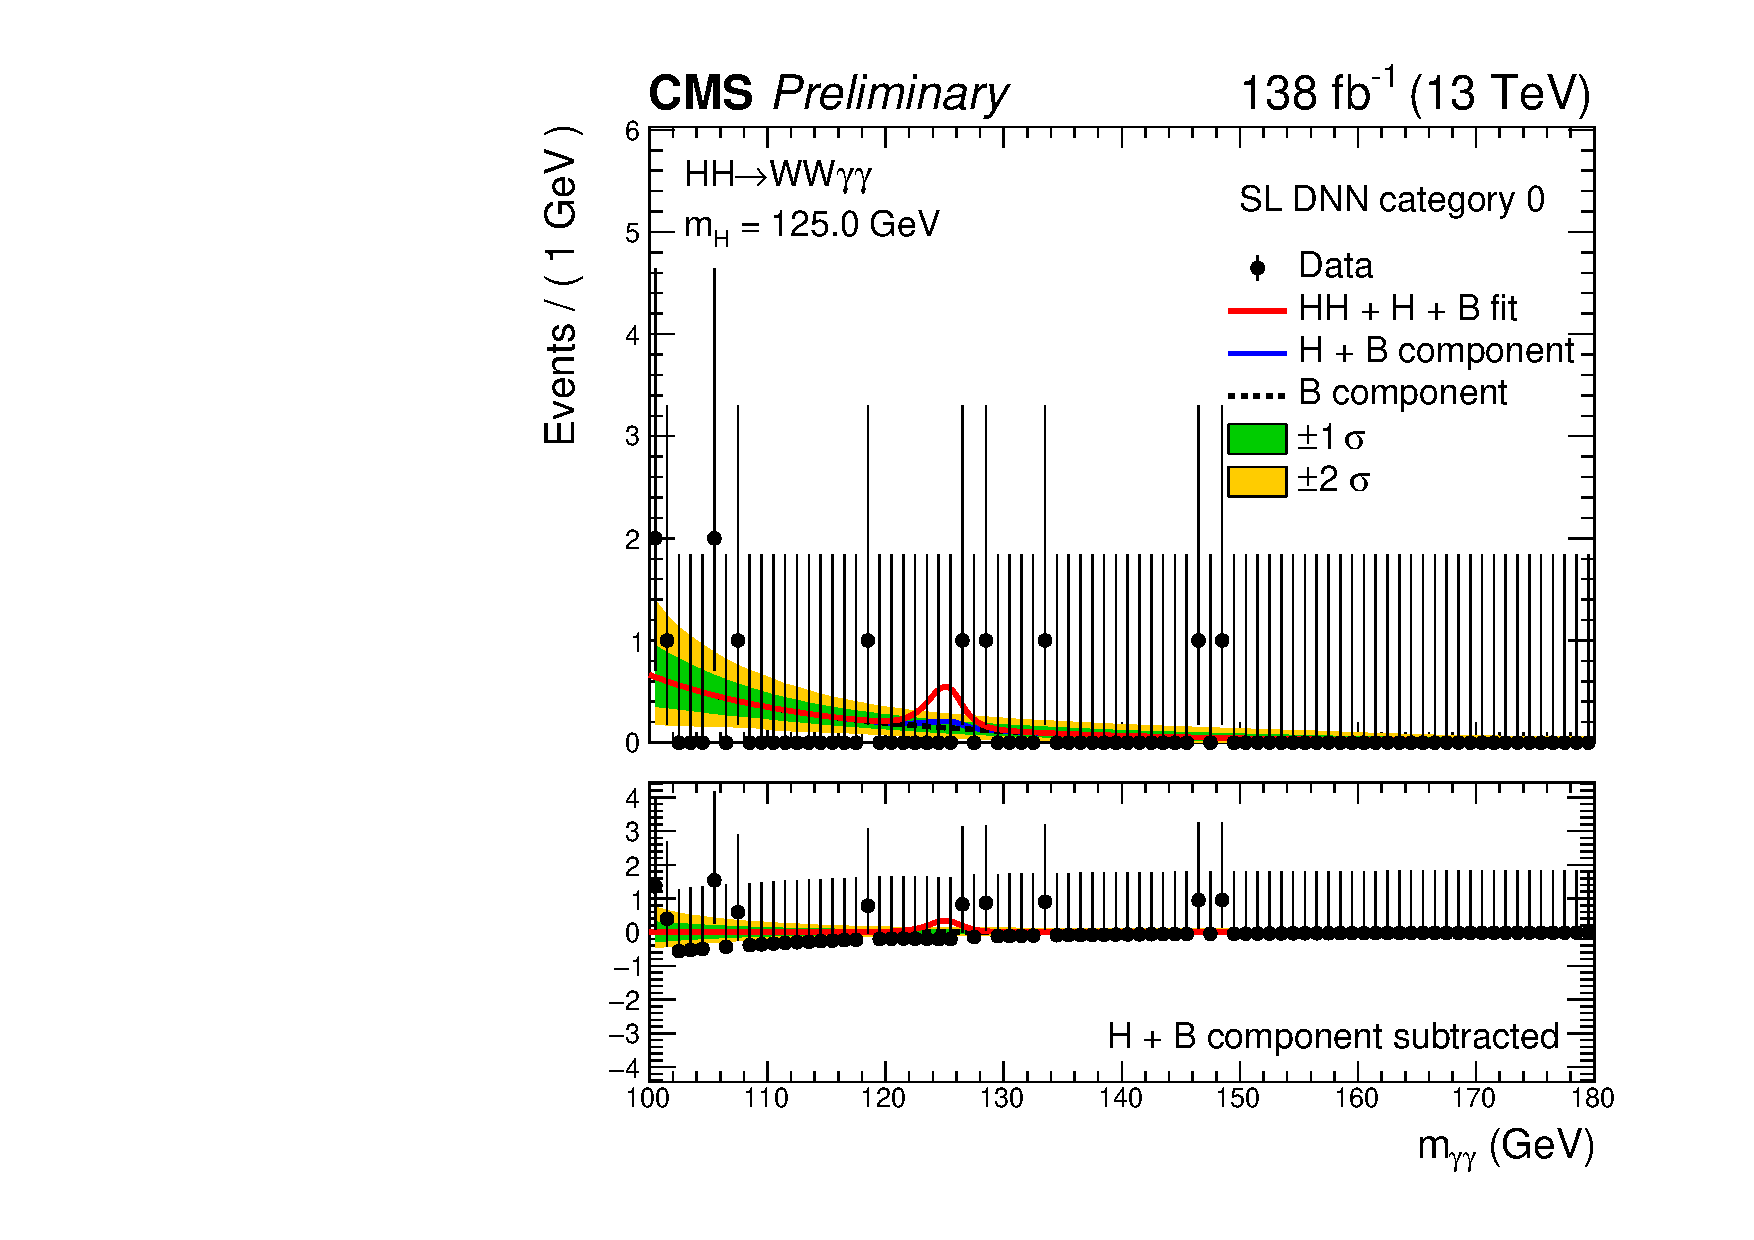
\includegraphics[width=0.45\textwidth]{Sections/HHWWgg/images/AnalyticFitting/SplusB/SLDNN_0_SplusB.pdf}}
    \caption{Semi-Leptonic data-driven background model for Run 2 data, DNN Category 0}
    \label{fig:SL_DataDrivenbkg_Run2_SLDNN_0}
\end{figure}

\begin{figure}[!htbp]

    \setcounter{subfigure}{0}
    \centering
    \subfloat[fTest]{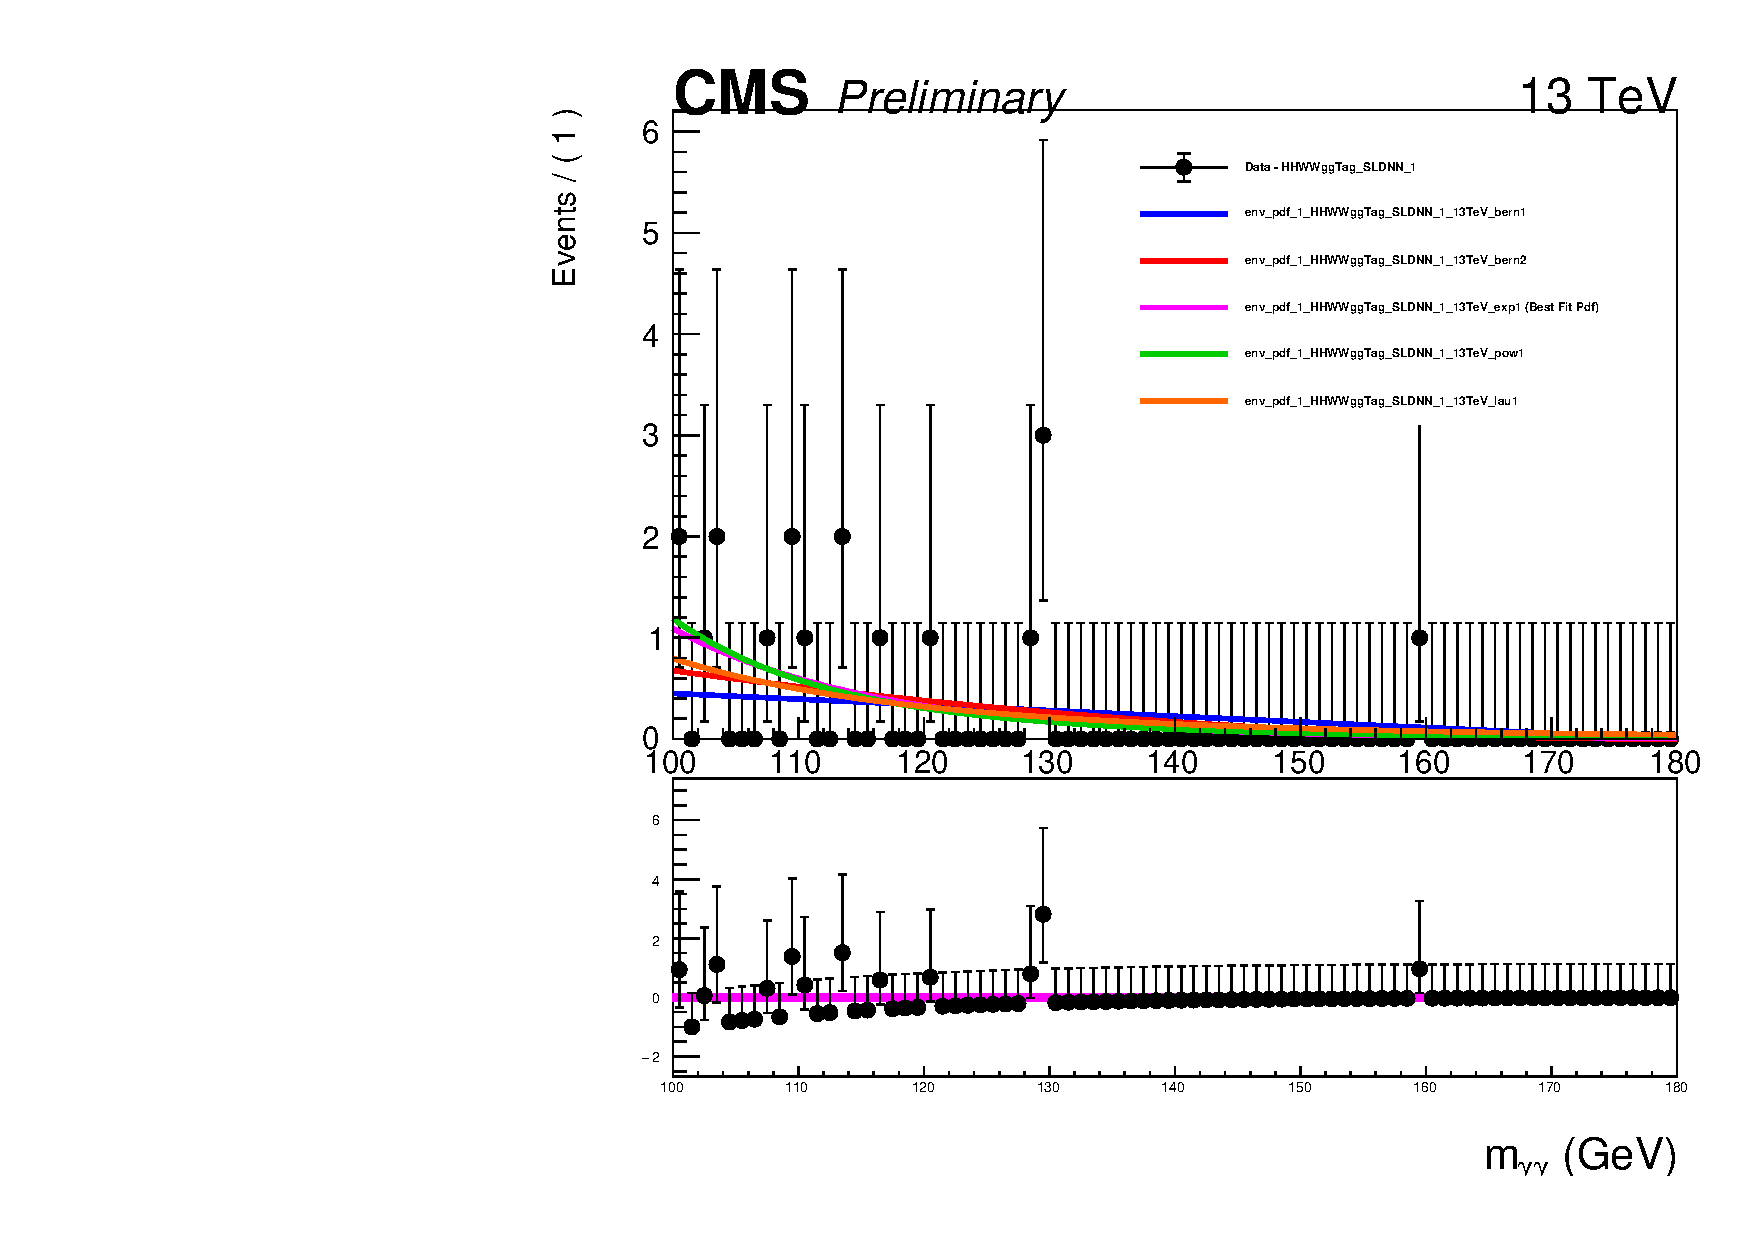
\includegraphics[width=0.45\textwidth]{Sections/HHWWgg/images/AnalyticFitting/ContinuumBackground/SL/Run2/multipdf_HHWWggTag_SLDNN_1.pdf}}
    \qquad
    \subfloat[Fit with uncertainty]{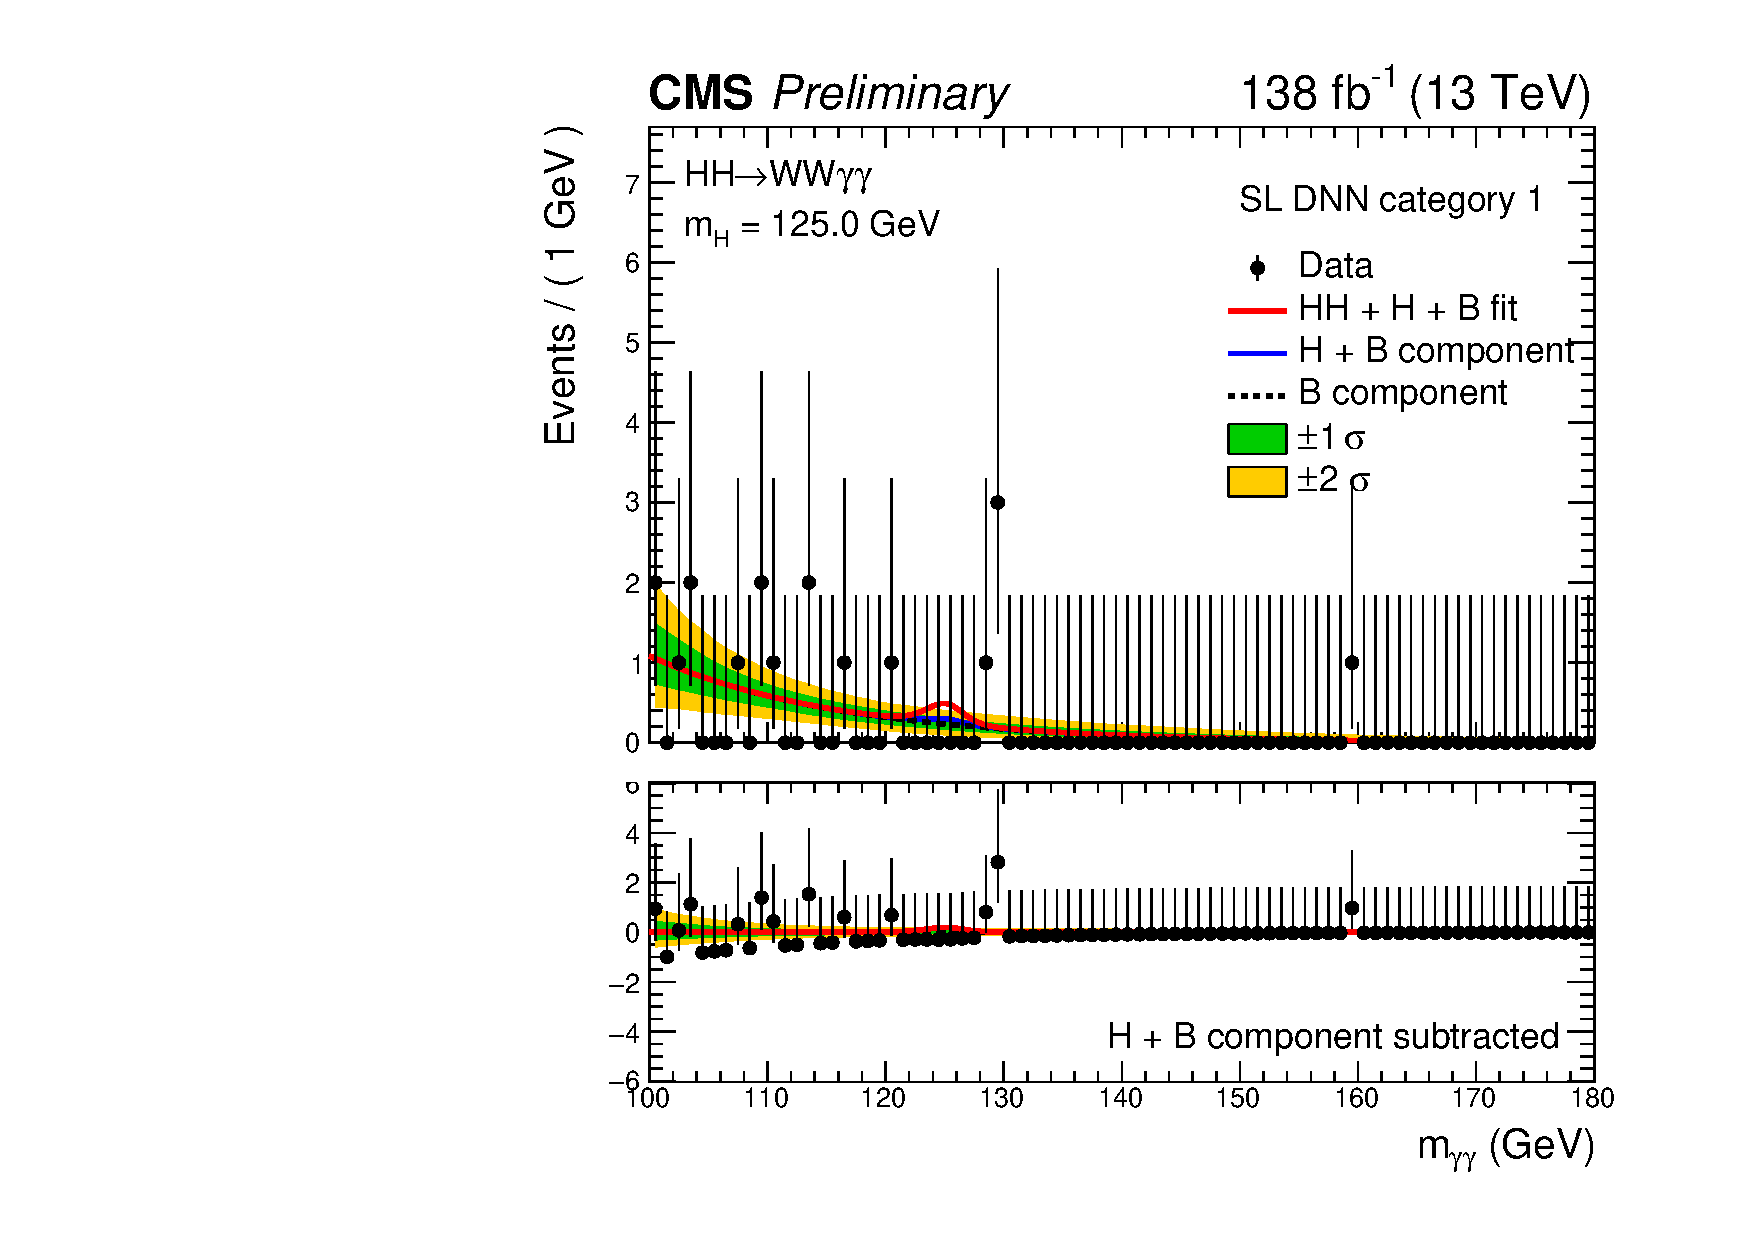
\includegraphics[width=0.45\textwidth]{Sections/HHWWgg/images/AnalyticFitting/SplusB/SLDNN_1_SplusB.pdf}}
    \caption{Semi-Leptonic data-driven background model for Run 2 data, DNN Category 1}
    \label{fig:SL_DataDrivenbkg_Run2_SLDNN_1}
\end{figure}

\begin{figure}[!htbp]

    \setcounter{subfigure}{0}
    \centering
    \subfloat[fTest]{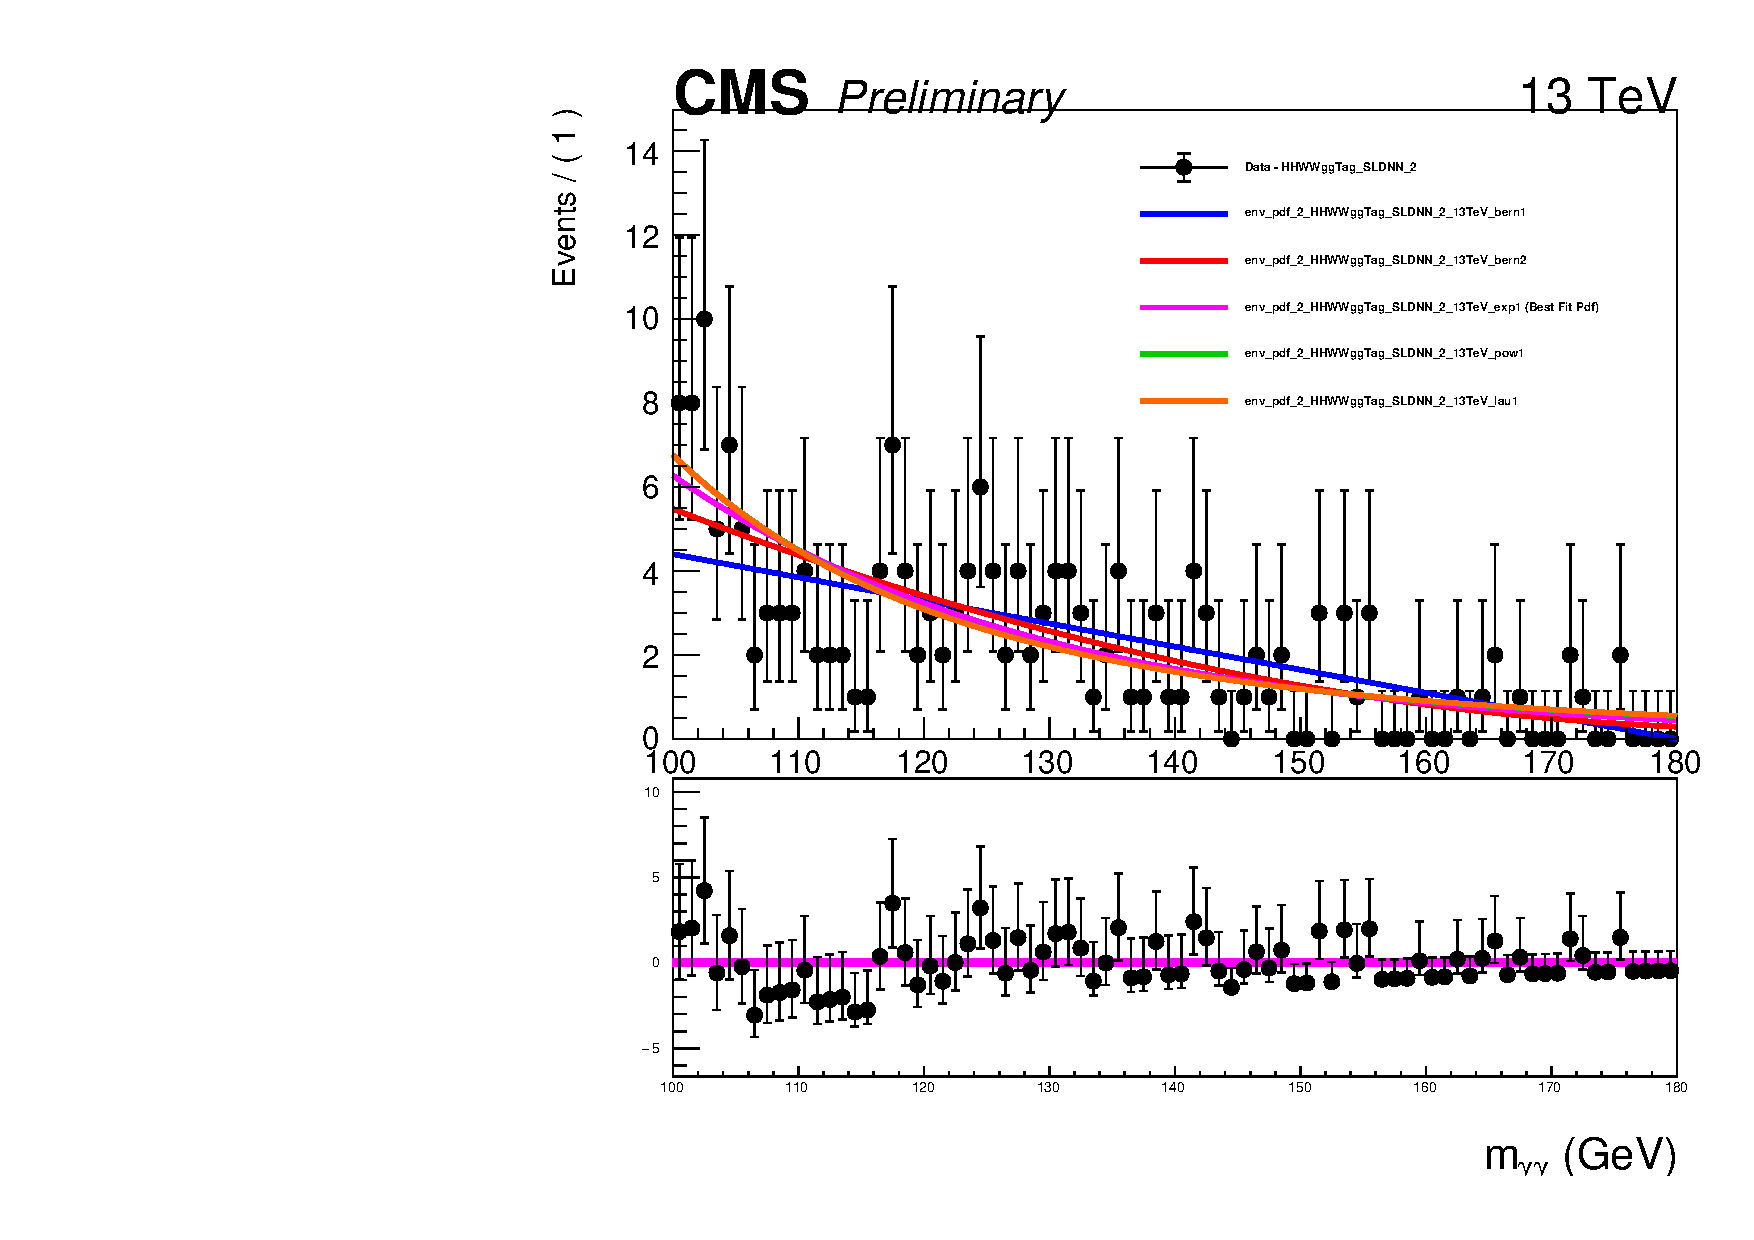
\includegraphics[width=0.45\textwidth]{Sections/HHWWgg/images/AnalyticFitting/ContinuumBackground/SL/Run2/multipdf_HHWWggTag_SLDNN_2.pdf}}
    \qquad
    \subfloat[Fit with uncertainty]{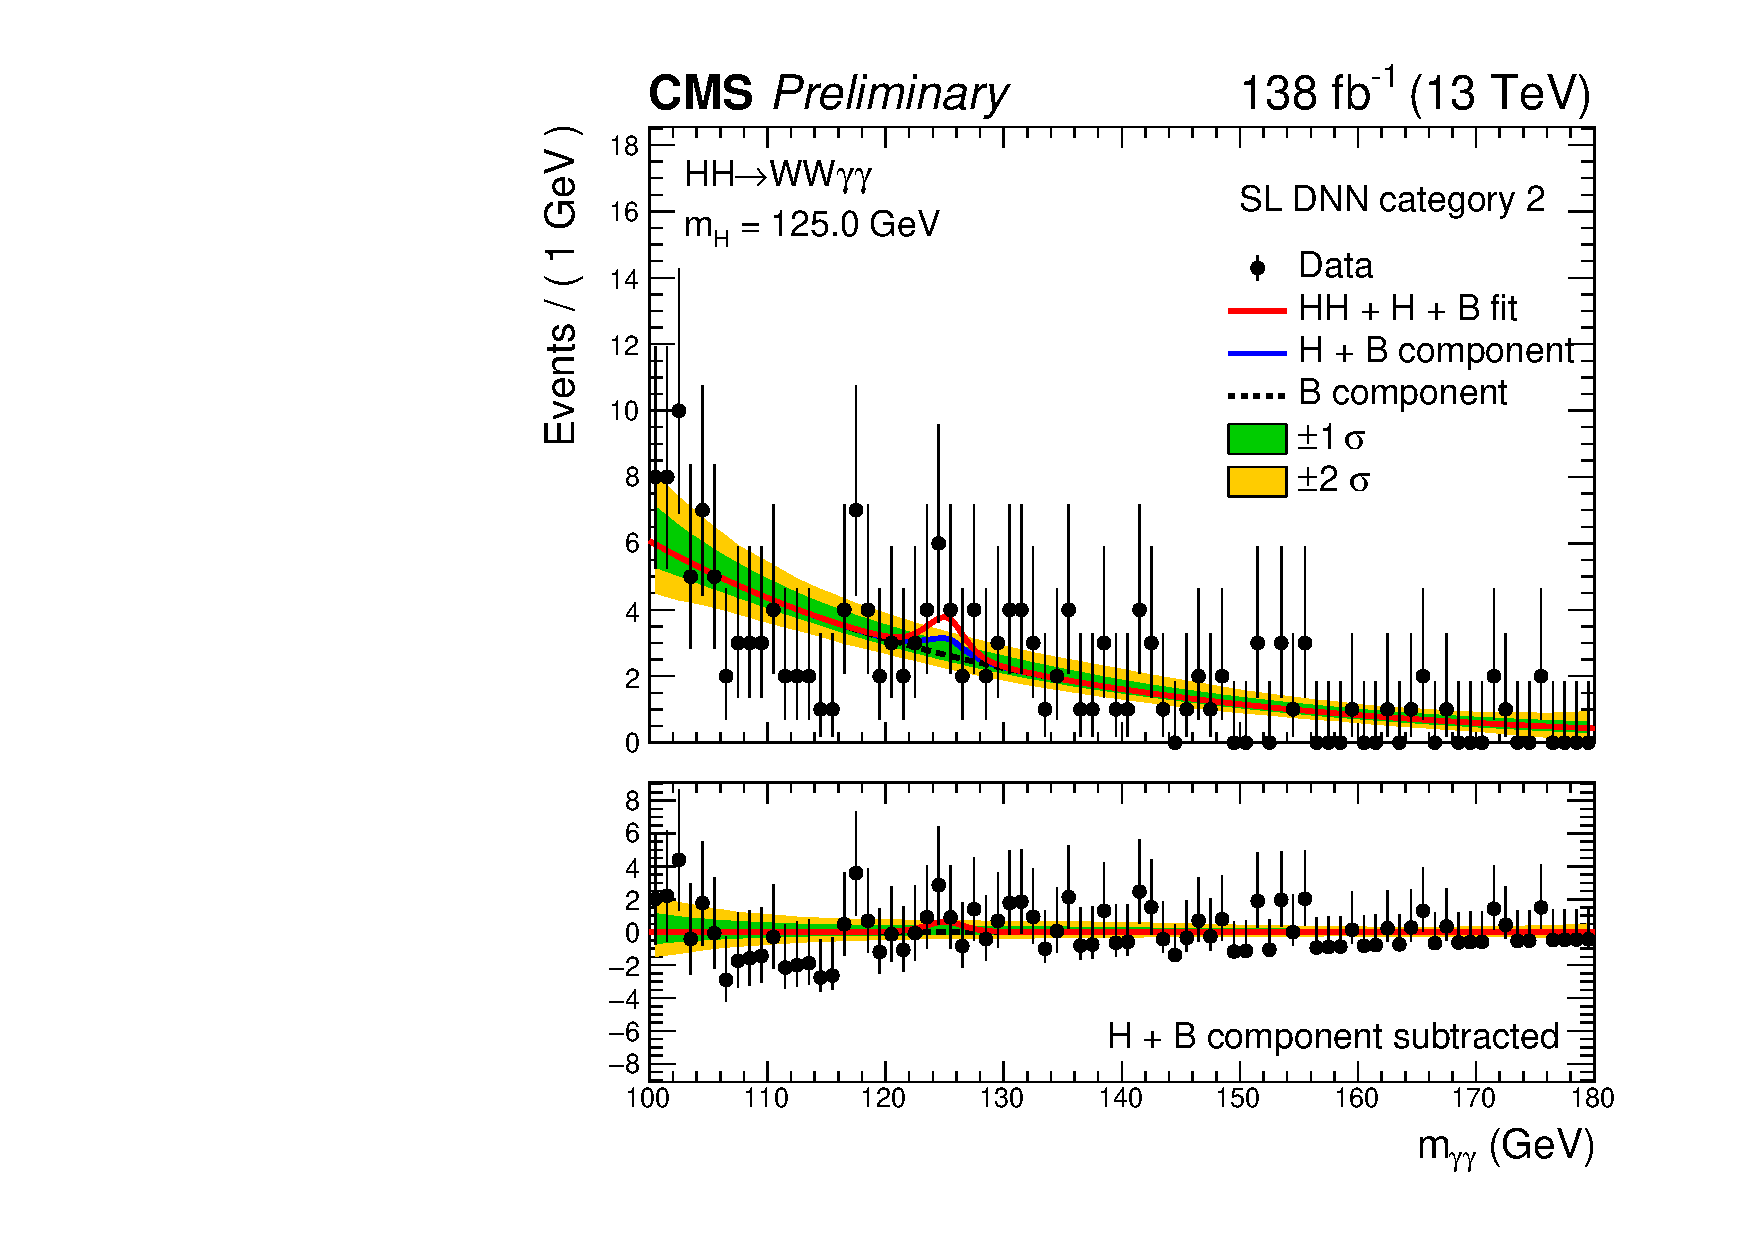
\includegraphics[width=0.45\textwidth]{Sections/HHWWgg/images/AnalyticFitting/SplusB/SLDNN_2_SplusB.pdf}}
    \caption{Semi-Leptonic data-driven background model for Run 2 data, DNN Category 2}
    \label{fig:SL_DataDrivenbkg_Run2_SLDNN_2}
\end{figure}

\begin{figure}[!htbp]

    \setcounter{subfigure}{0}
    \centering
    \subfloat[fTest]{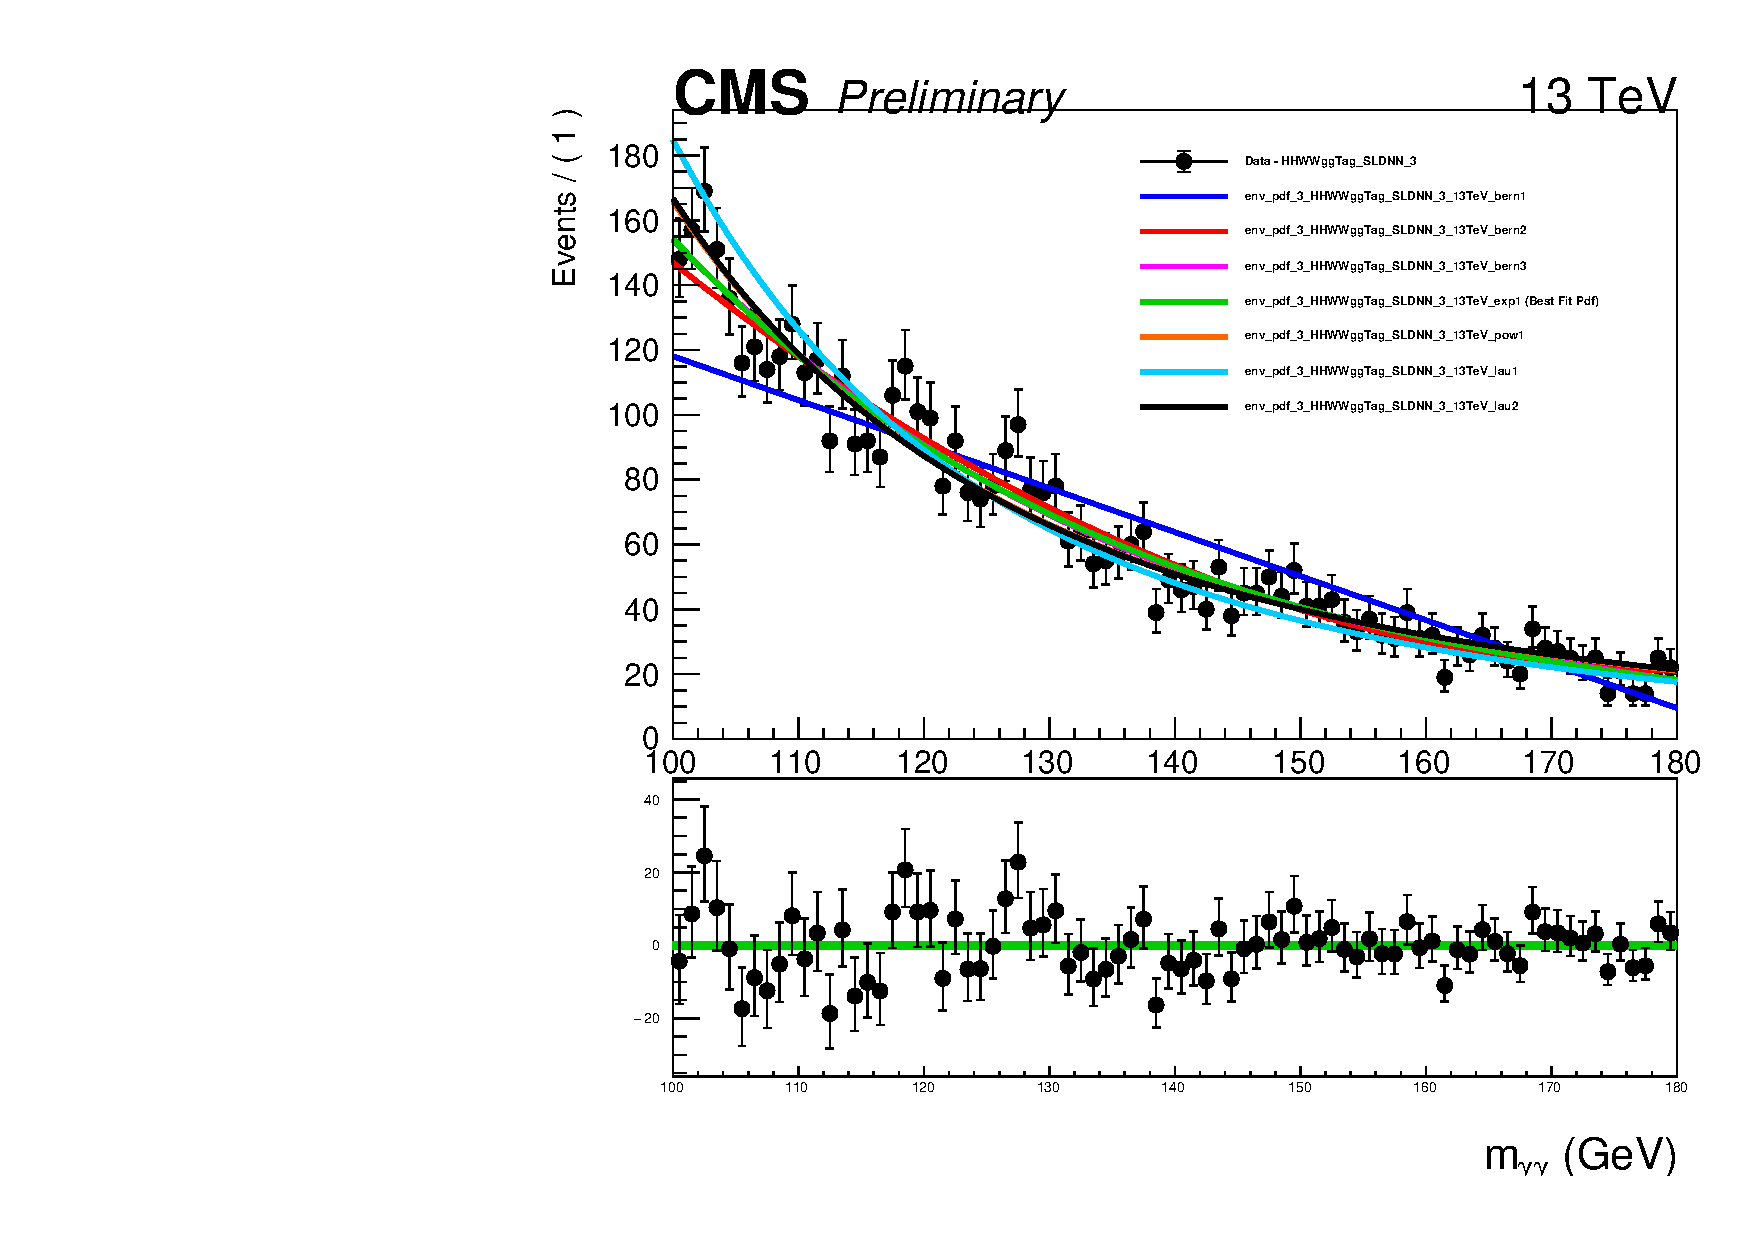
\includegraphics[width=0.45\textwidth]{Sections/HHWWgg/images/AnalyticFitting/ContinuumBackground/SL/Run2/multipdf_HHWWggTag_SLDNN_3.pdf}}
    \qquad
    \subfloat[Fit with uncertainty]{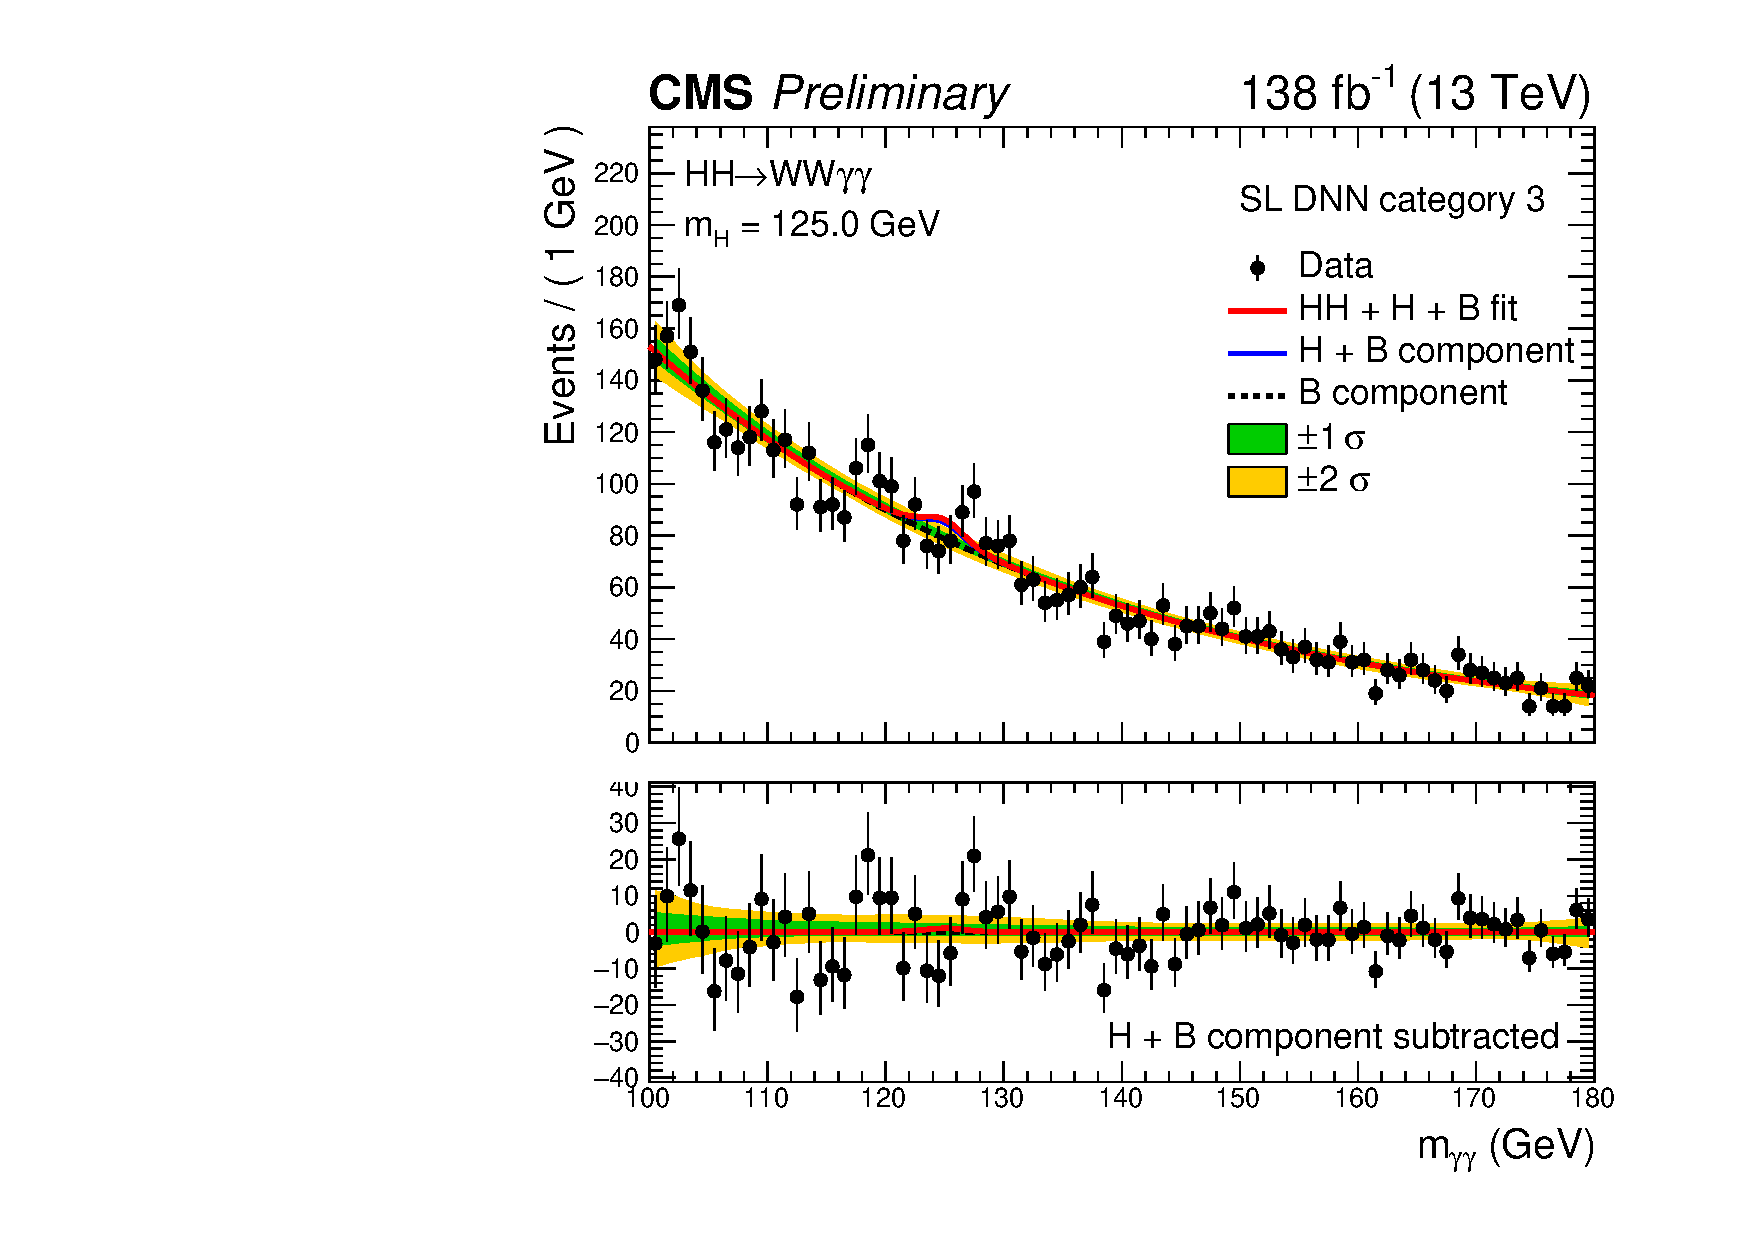
\includegraphics[width=0.45\textwidth]{Sections/HHWWgg/images/AnalyticFitting/SplusB/SLDNN_3_SplusB.pdf}}
    \caption{Semi-Leptonic data-driven background model for Run 2 data, DNN Category 3}
    \label{fig:SL_DataDrivenbkg_Run2_SLDNN_3}
\end{figure}

\begin{figure}[!htbp]
% \vspace{-1cm}
    \setcounter{subfigure}{0}

    \subfloat[fTest, DNN Category 2]{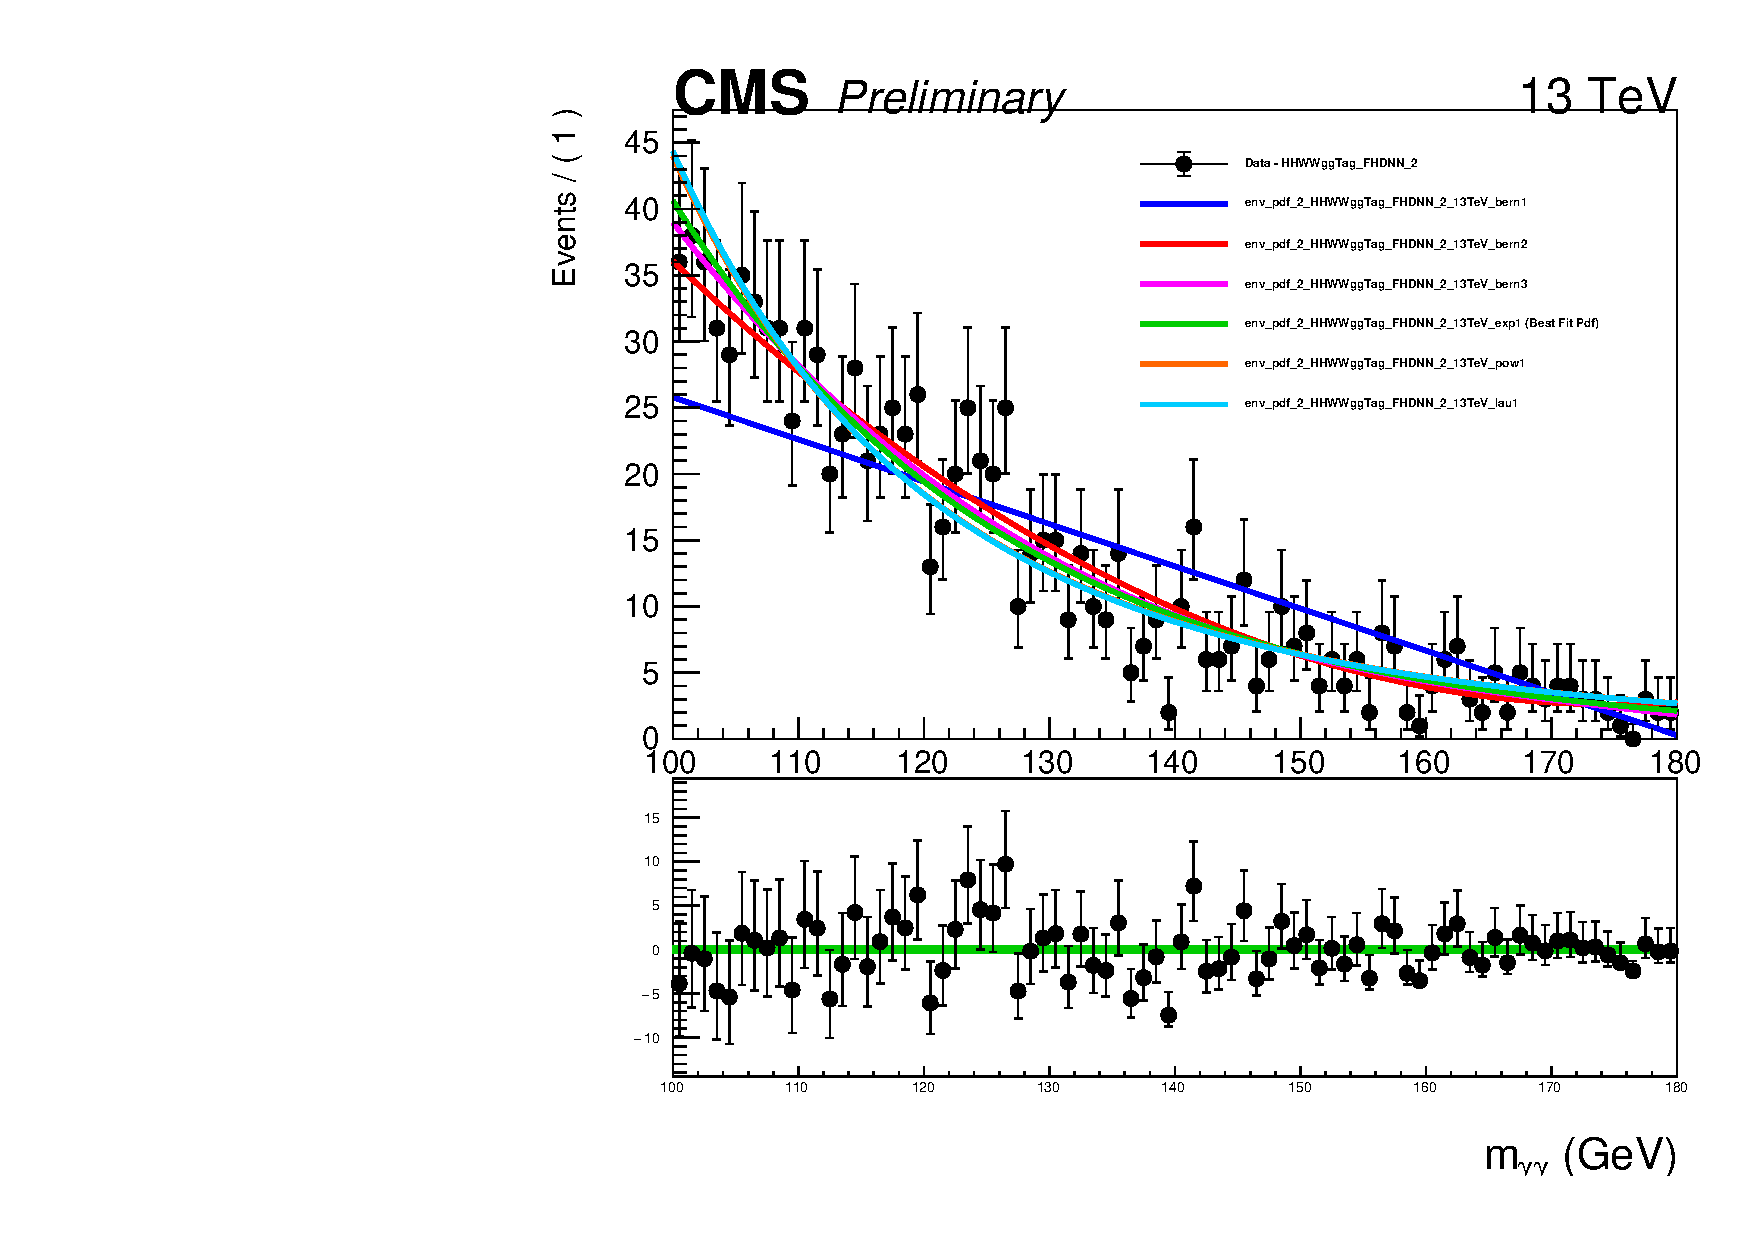
\includegraphics[width=0.45\textwidth]{Sections/HHWWgg/images/AnalyticFitting/ContinuumBackground/FullyHadronic/multipdf_HHWWggTag_FHDNN_2.pdf}}
    \qquad
    \subfloat[Background Fit, DNN Category 2]{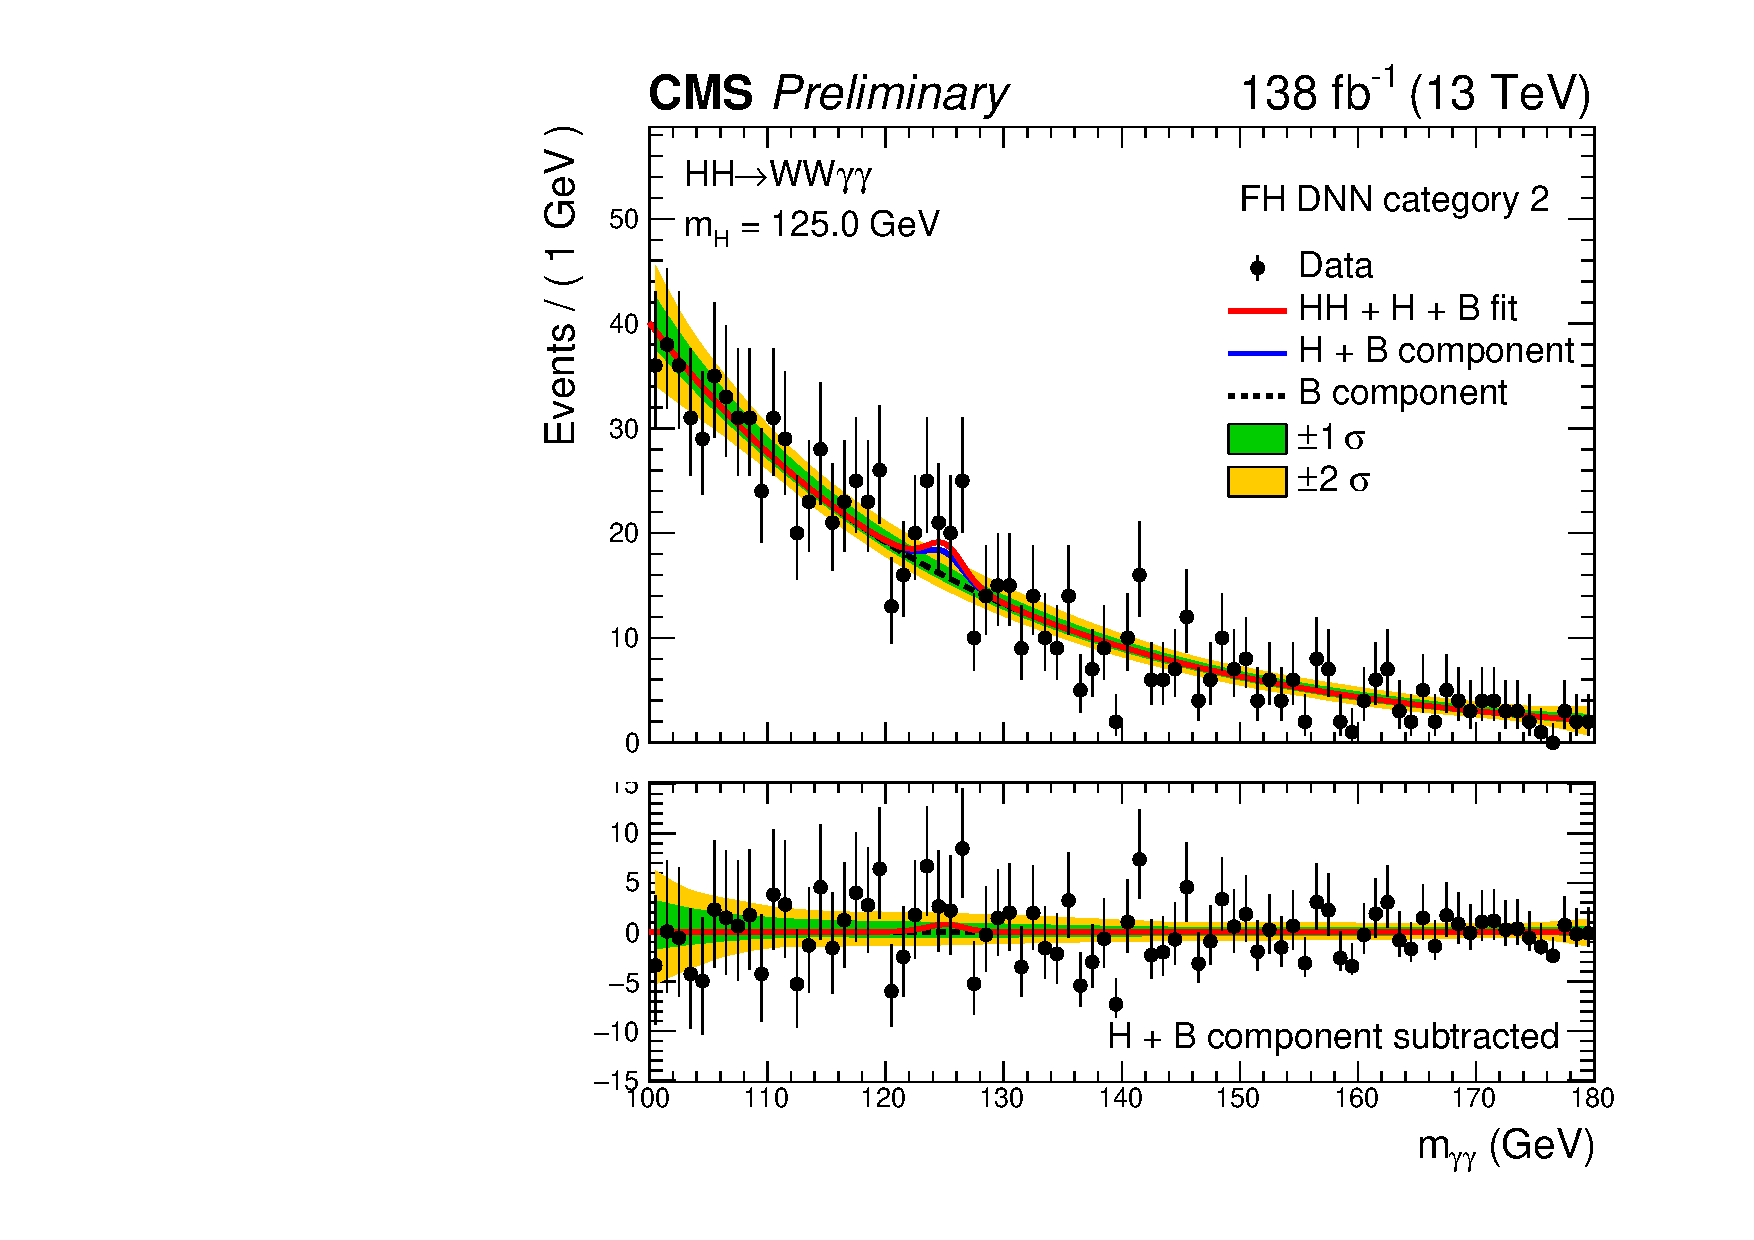
\includegraphics[width=0.45\textwidth]{Sections/HHWWgg/images/AnalyticFitting/SplusB/FHDNN_2_SplusB.pdf}}
    \caption{Fully-Hadronic data-driven background models for Run 2 data \label{fig:FH_SidebandFits}}
\end{figure}


\begin{figure}[!htbp]
    \setcounter{subfigure}{0}
    \centering
    \subfloat[fTest, DNN category 0]{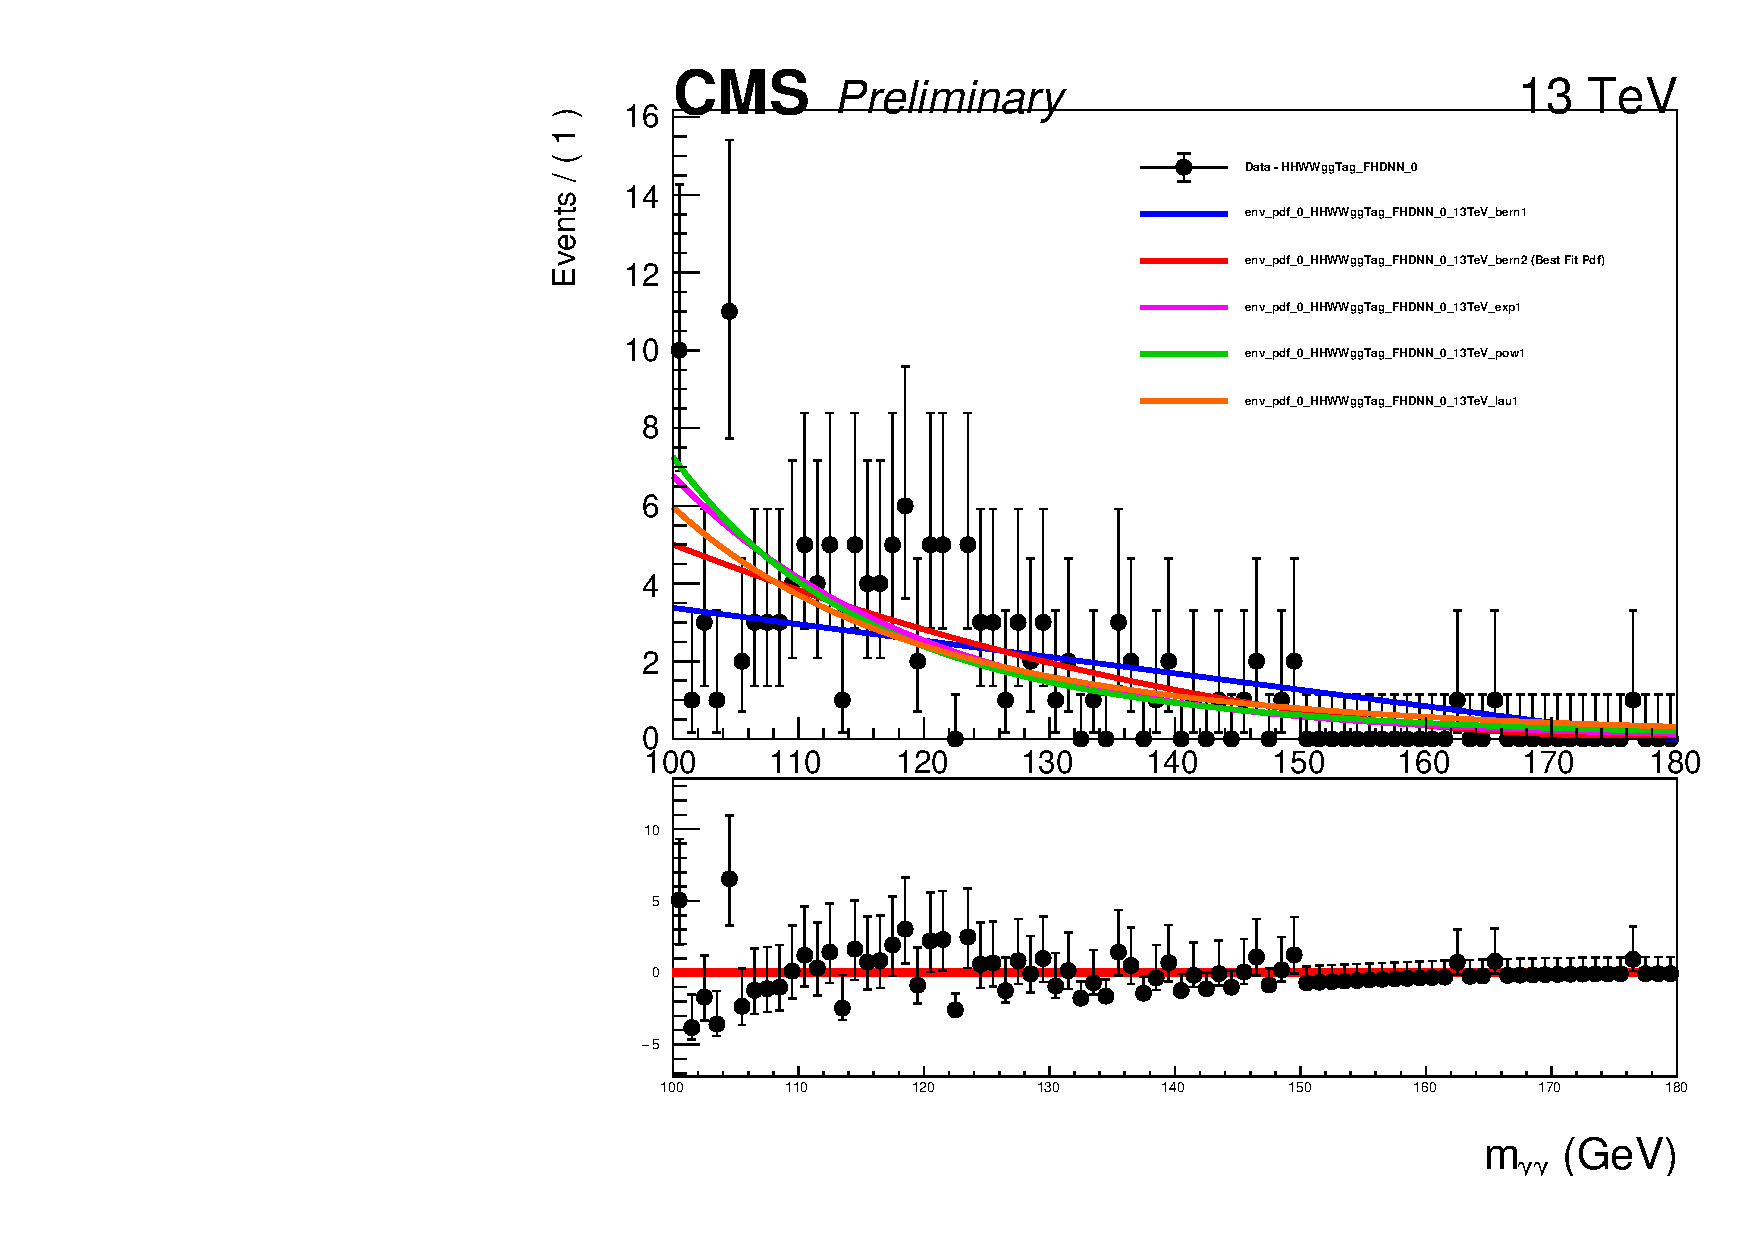
\includegraphics[width=0.45\textwidth]{Sections/HHWWgg/images/AnalyticFitting/ContinuumBackground/FullyHadronic/multipdf_HHWWggTag_FHDNN_0.pdf}}
    \qquad
    \subfloat[B $+$ S fit to data, category 0]{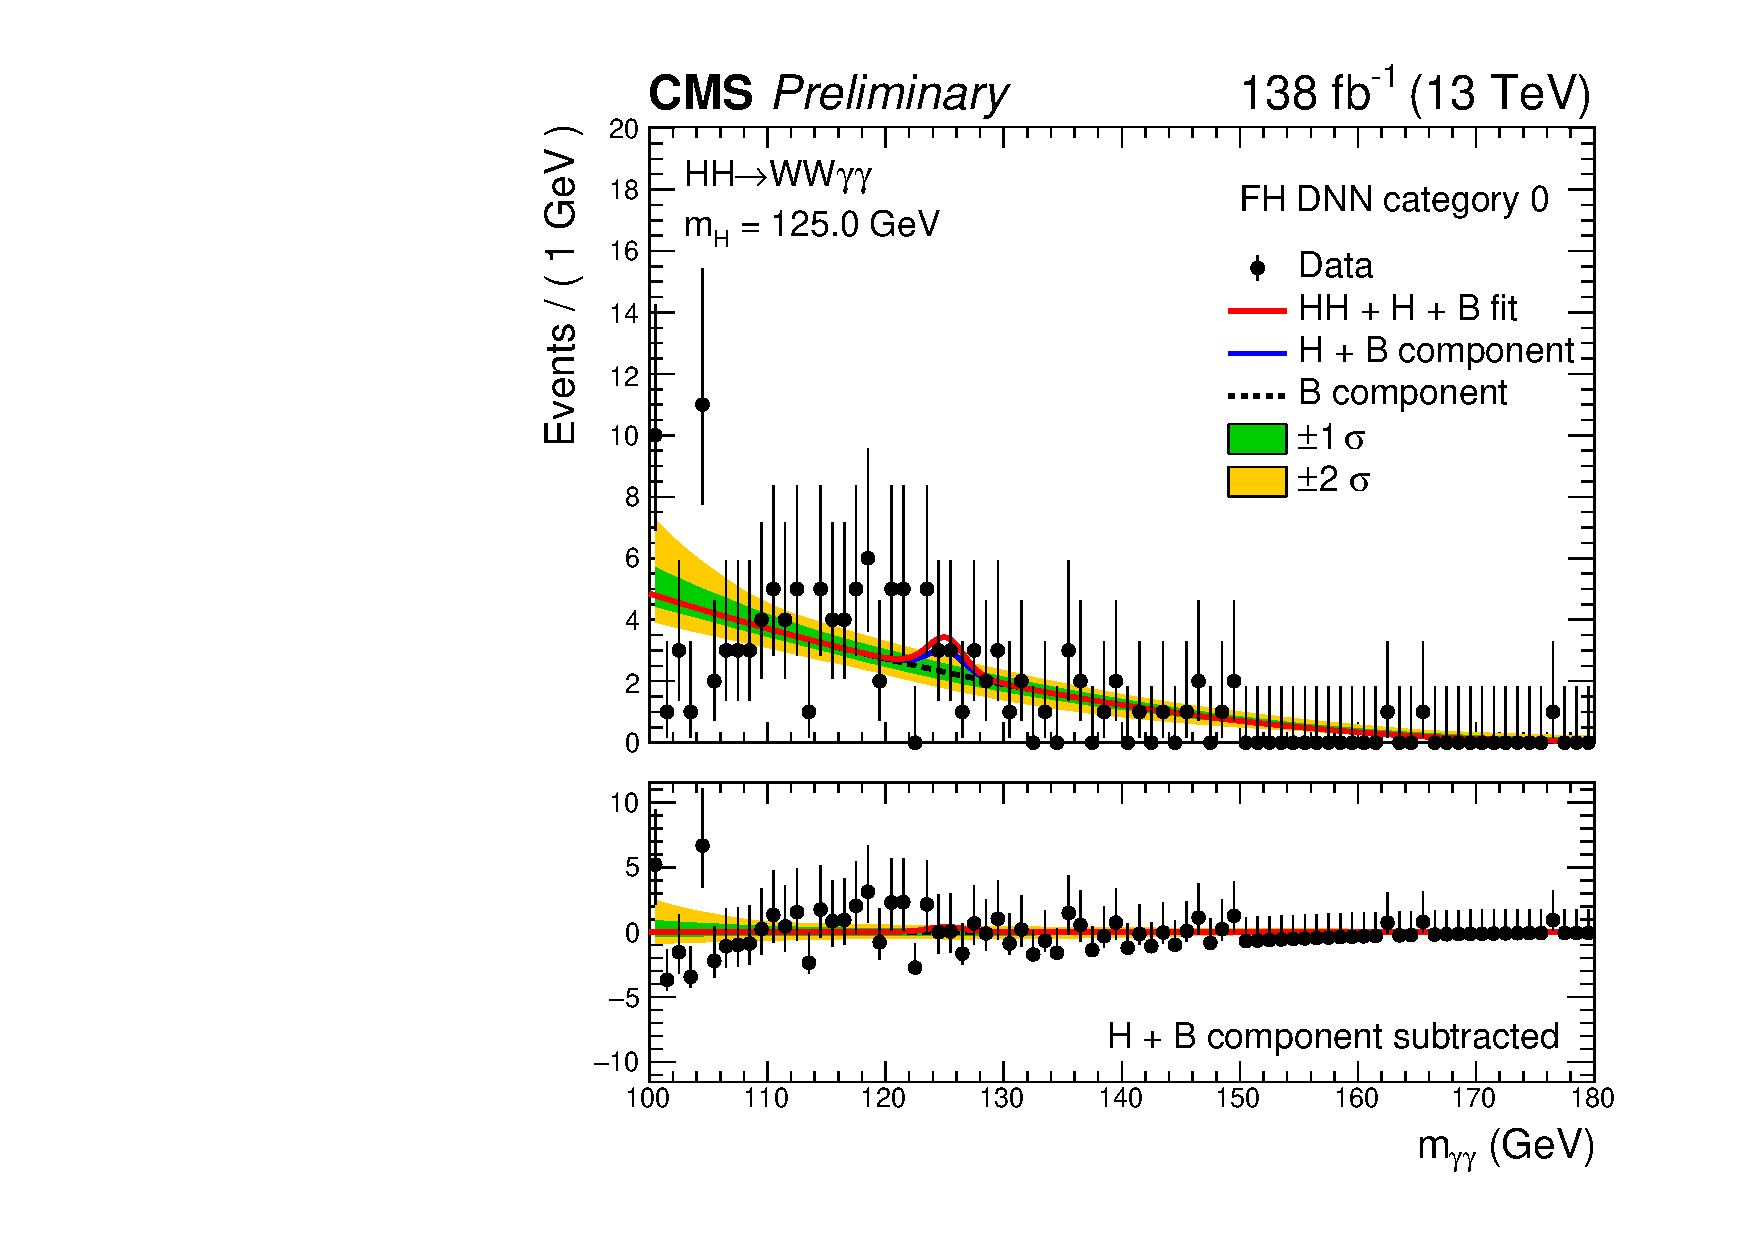
\includegraphics[width=0.45\textwidth]{Sections/HHWWgg/images/AnalyticFitting/SplusB/FHDNN_0_SplusB.pdf}}
    \caption{Fully-Hadronic data-driven background and simulation models}
    \label{fig:FH_SidebandFits_1}
\end{figure}

\begin{figure}[!htbp]
    \setcounter{subfigure}{0}
    \centering
    \subfloat[fTest, DNN category 1]{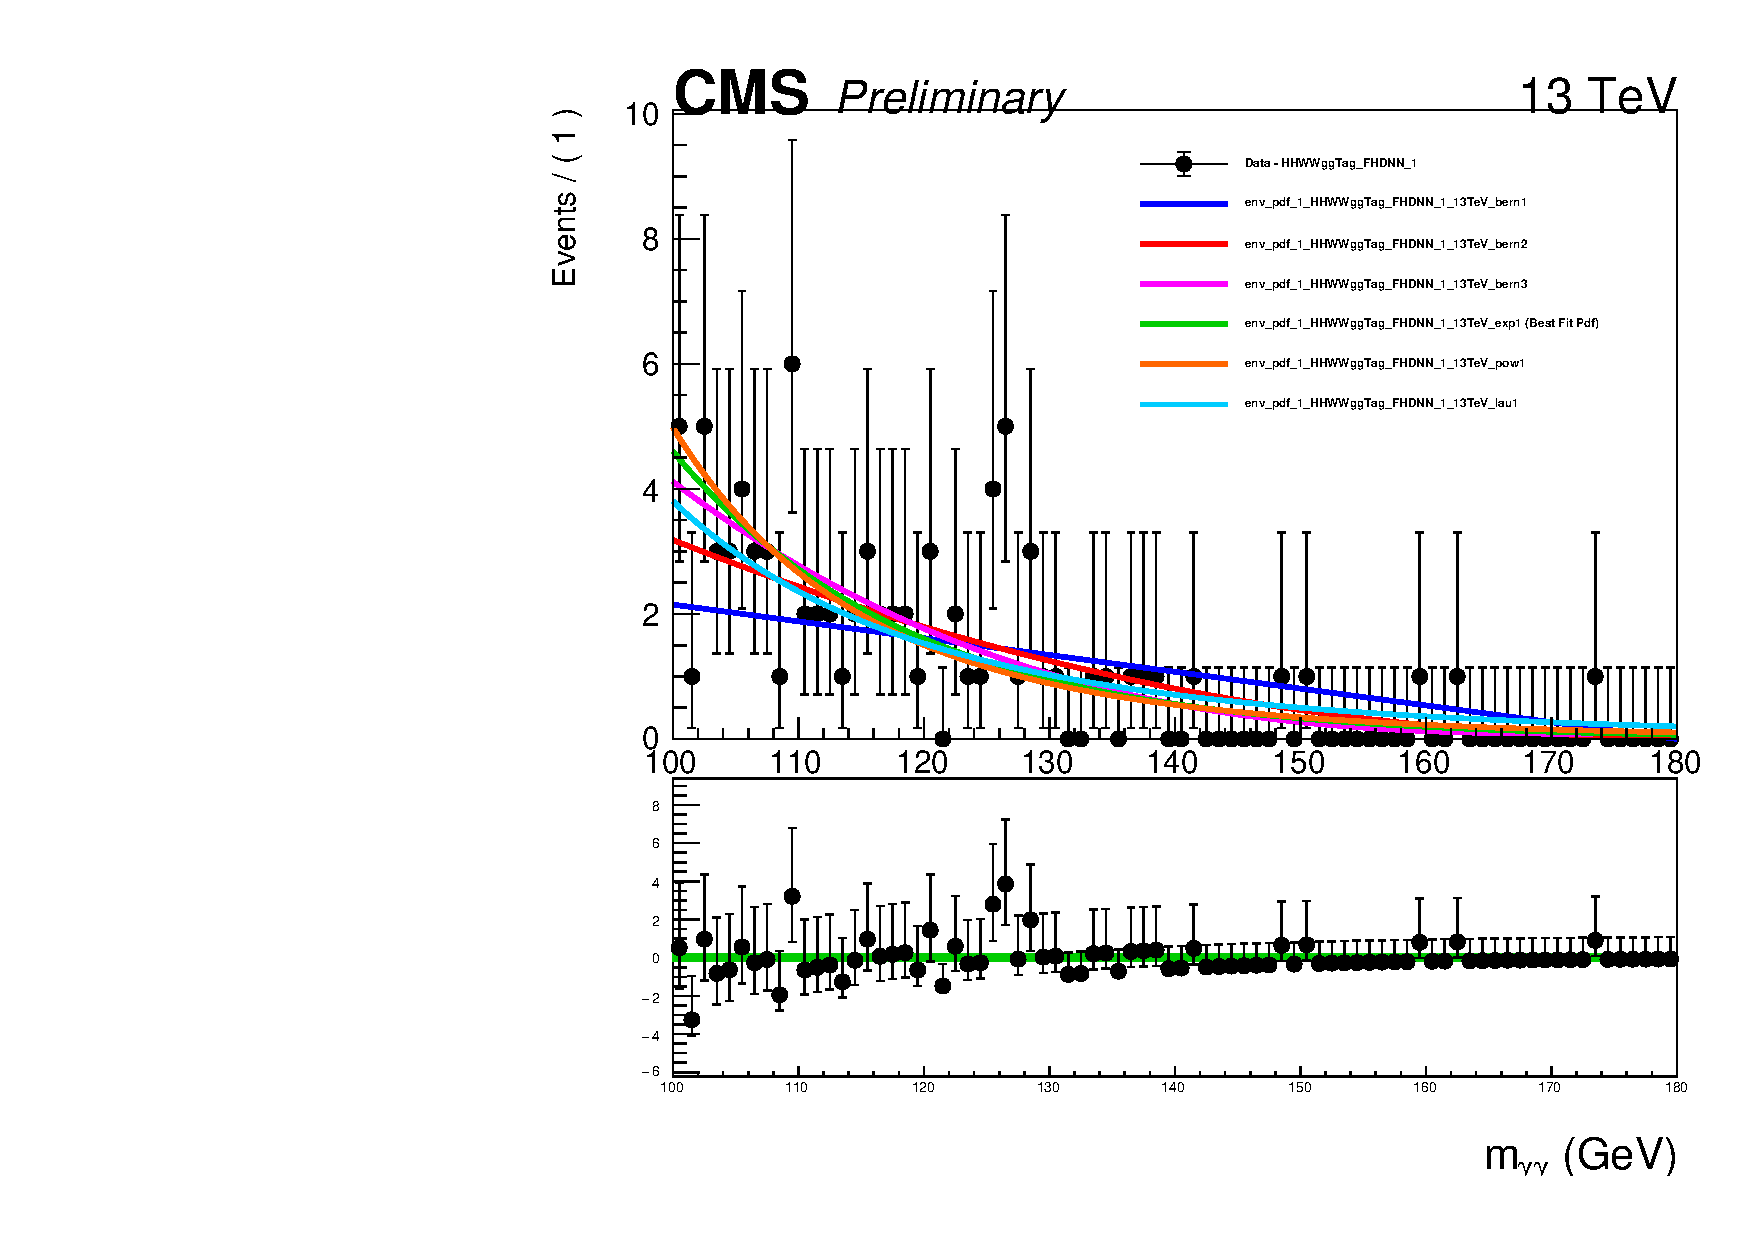
\includegraphics[width=0.45\textwidth]{Sections/HHWWgg/images/AnalyticFitting/ContinuumBackground/FullyHadronic/multipdf_HHWWggTag_FHDNN_1.pdf}}
    \qquad
    \subfloat[B $+$ S fit to data, category 1]{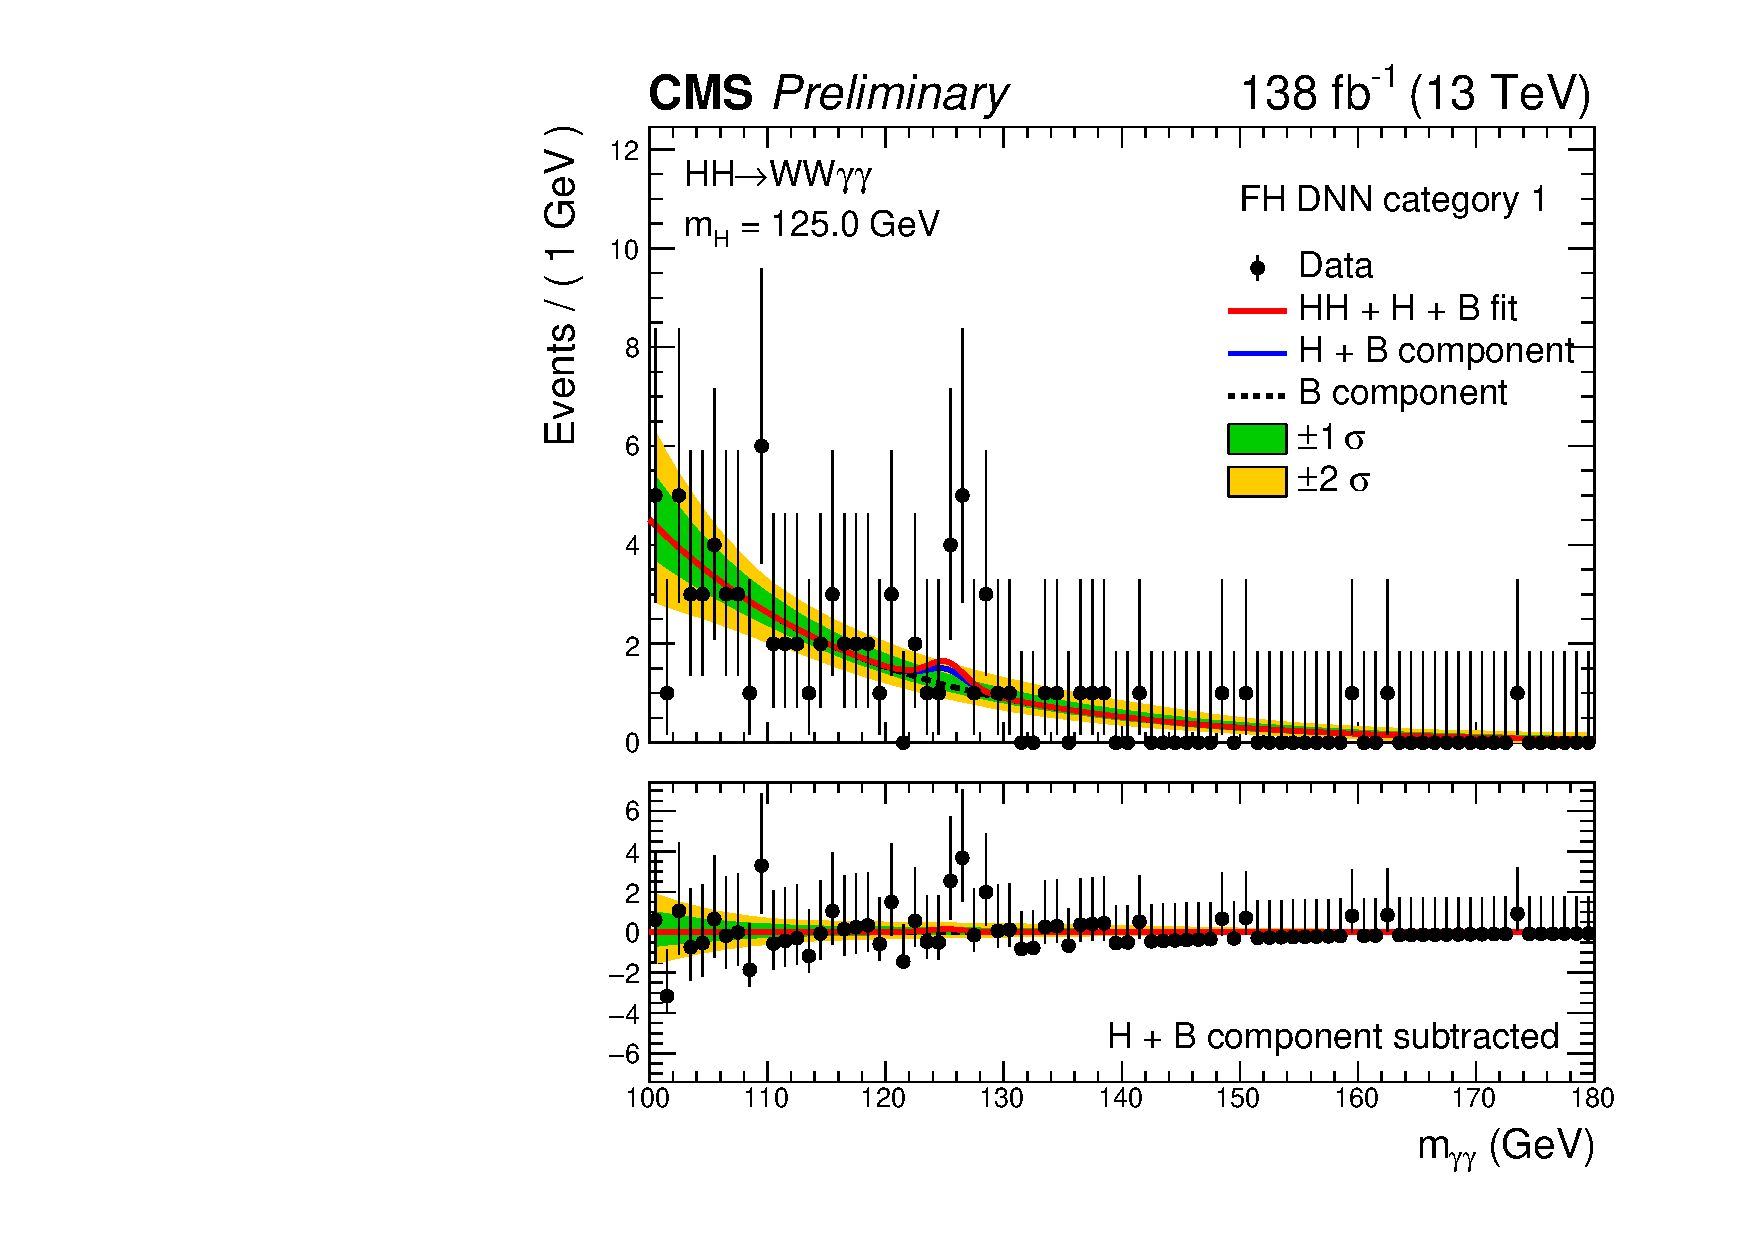
\includegraphics[width=0.45\textwidth]{Sections/HHWWgg/images/AnalyticFitting/SplusB/FHDNN_1_SplusB.pdf}}
    \caption{Fully-Hadronic data-driven background and simulation models}
    \label{fig:FH_SidebandFits_2}
\end{figure}

\begin{figure}[!htbp]
    \setcounter{subfigure}{0}
    \centering
    \subfloat[fTest, DNN category 2]{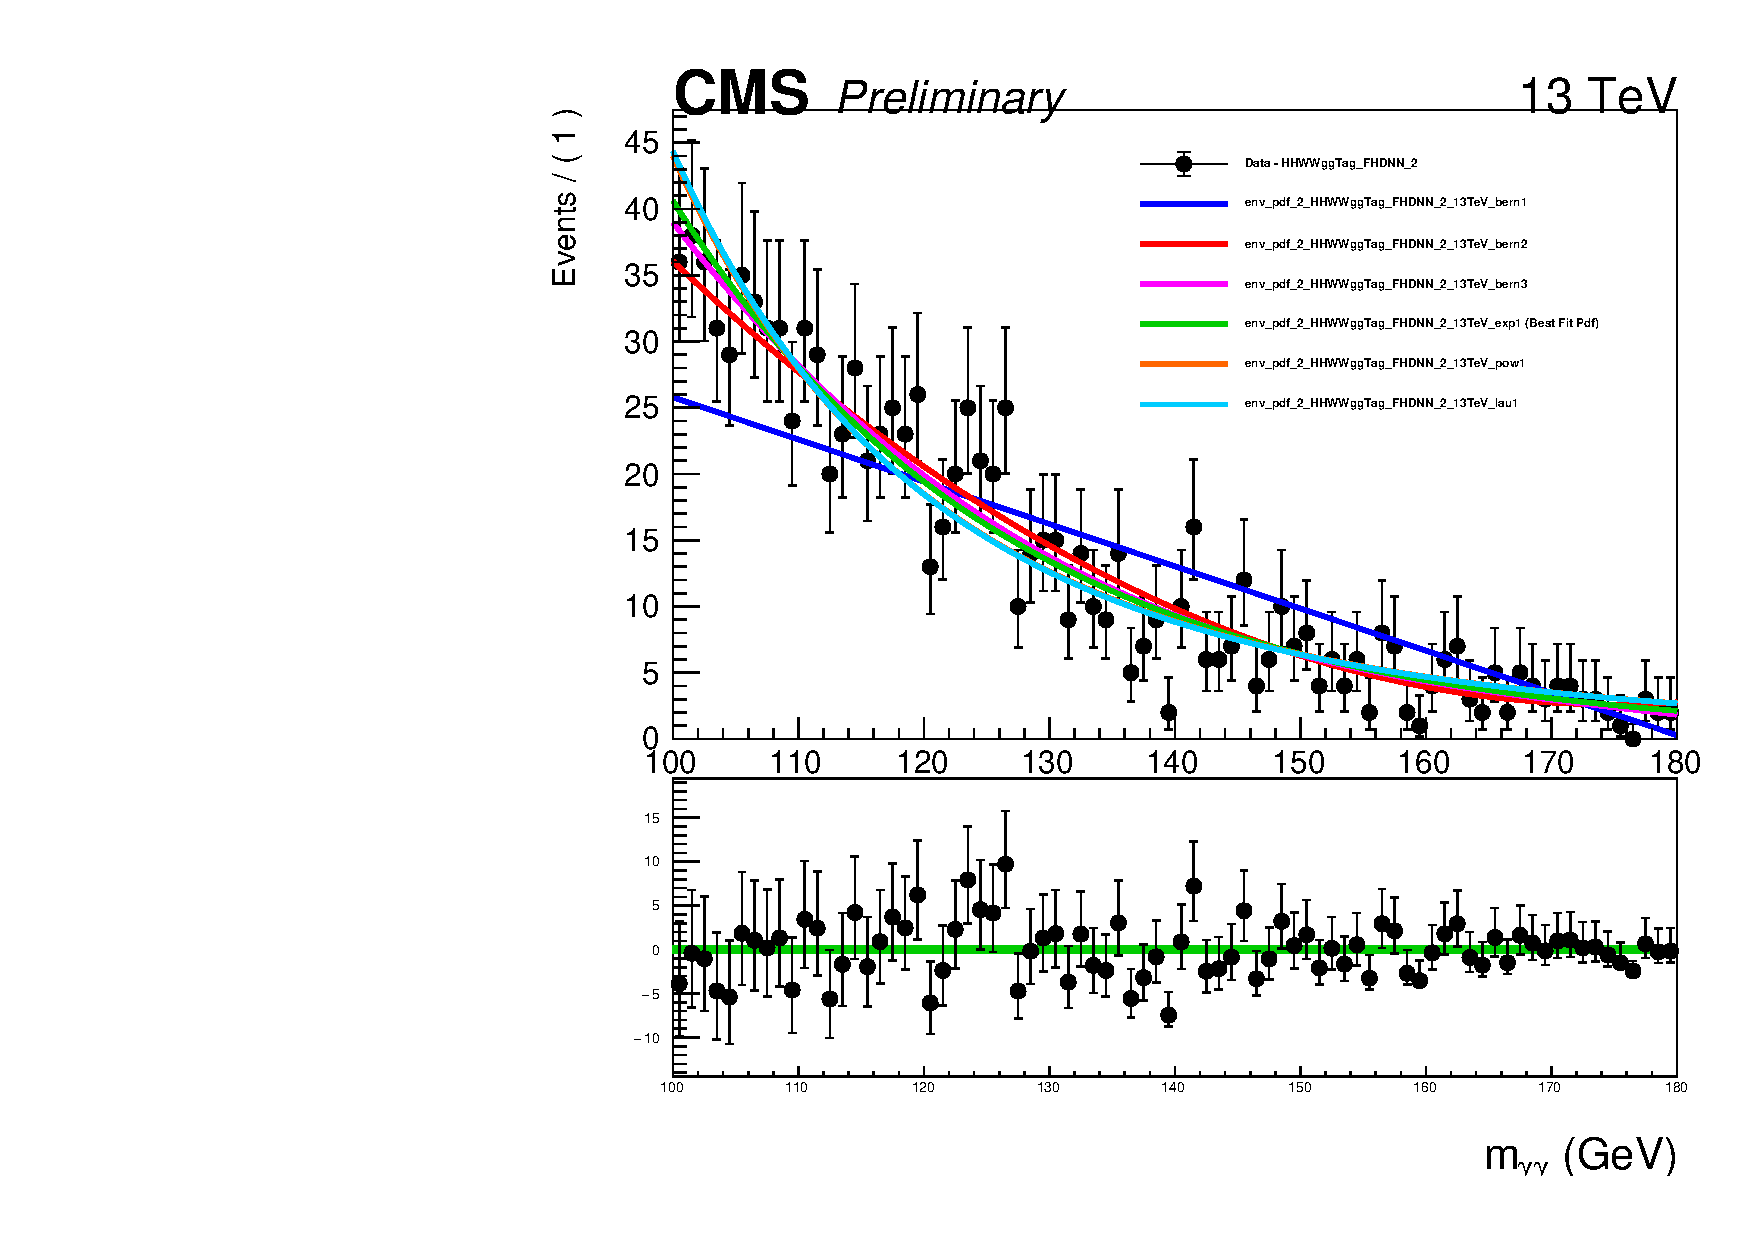
\includegraphics[width=0.45\textwidth]{Sections/HHWWgg/images/AnalyticFitting/ContinuumBackground/FullyHadronic/multipdf_HHWWggTag_FHDNN_2.pdf}}
    \qquad
    \subfloat[B $+$ S fit to data, category 2]{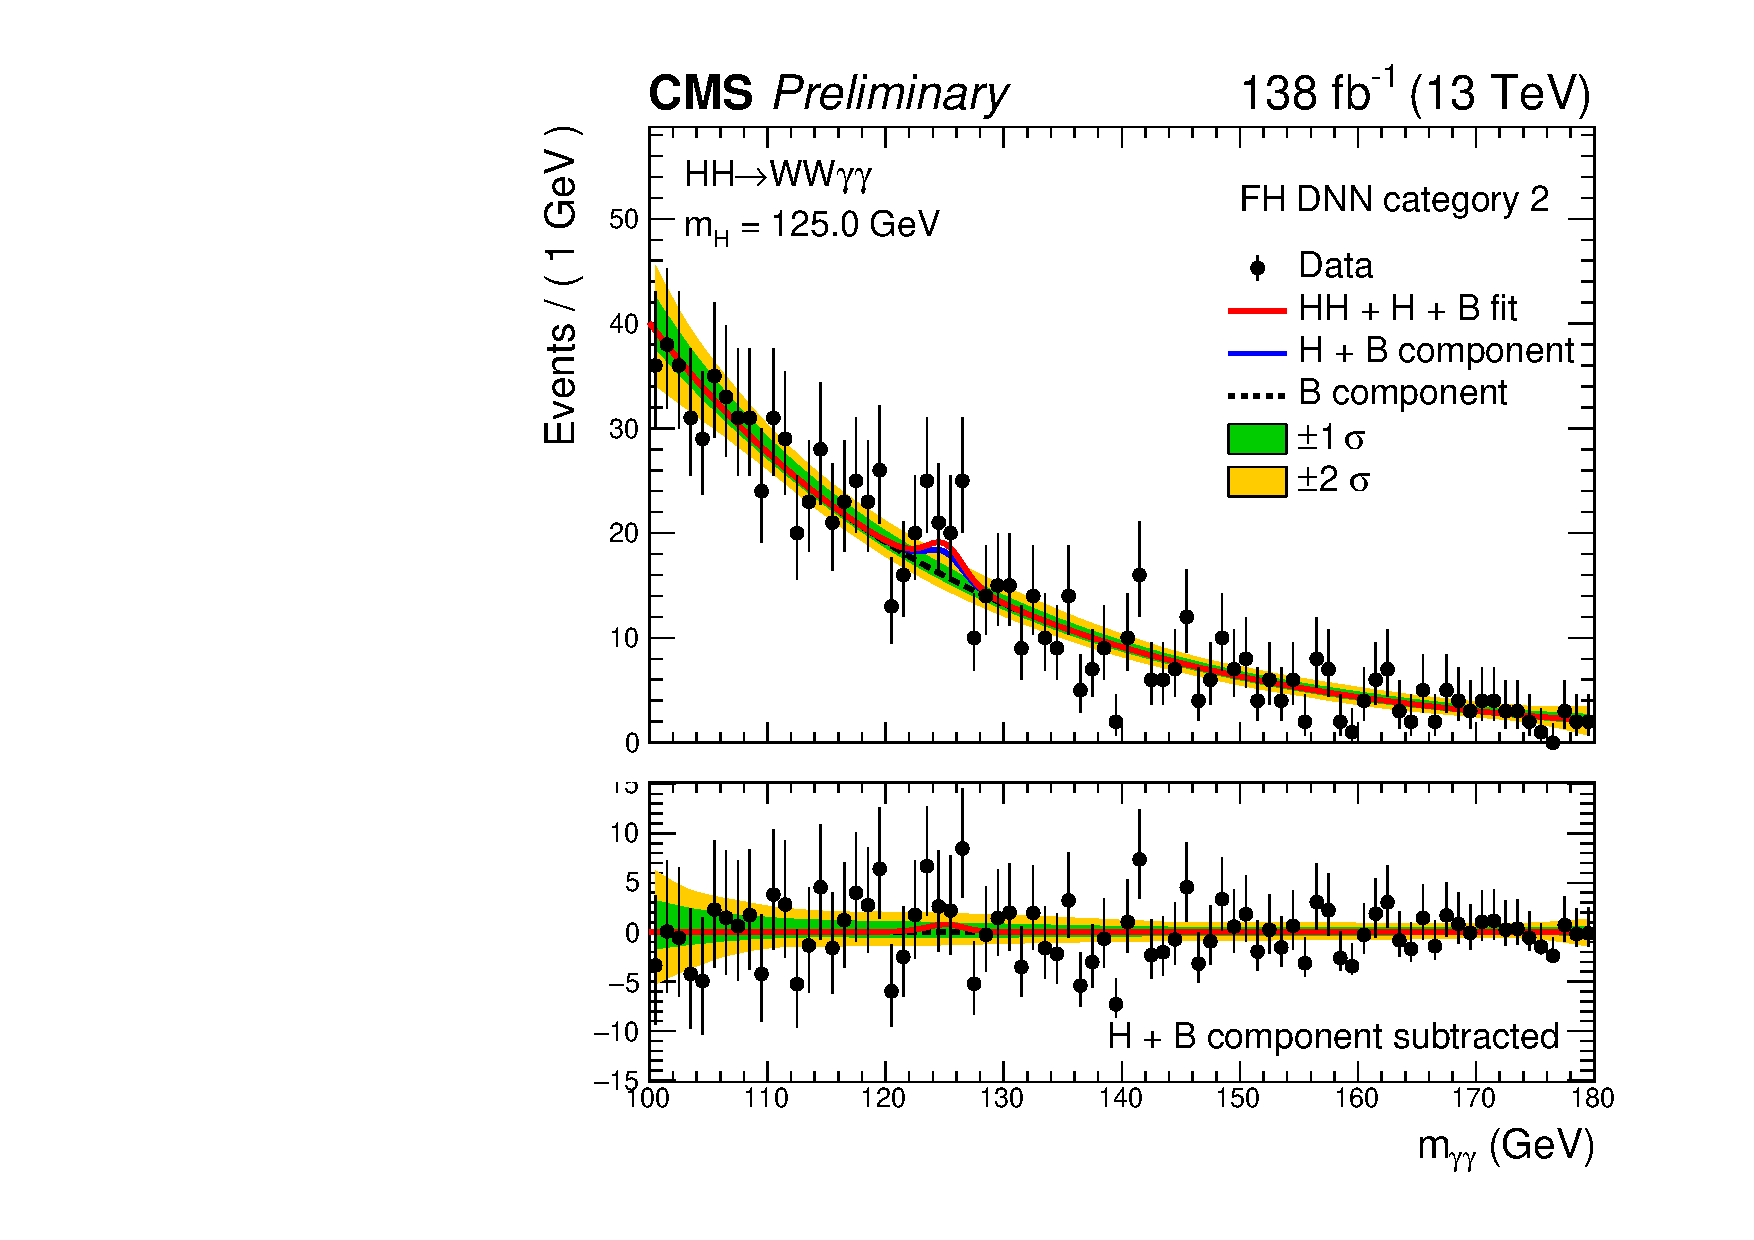
\includegraphics[width=0.45\textwidth]{Sections/HHWWgg/images/AnalyticFitting/SplusB/FHDNN_2_SplusB.pdf}}
    \caption{Fully-Hadronic data-driven background and simulation models}
    \label{fig:FH_SidebandFits_2}
\end{figure}

\begin{figure}[!htbp]
    \setcounter{subfigure}{0}
    \centering
    \subfloat[fTest]{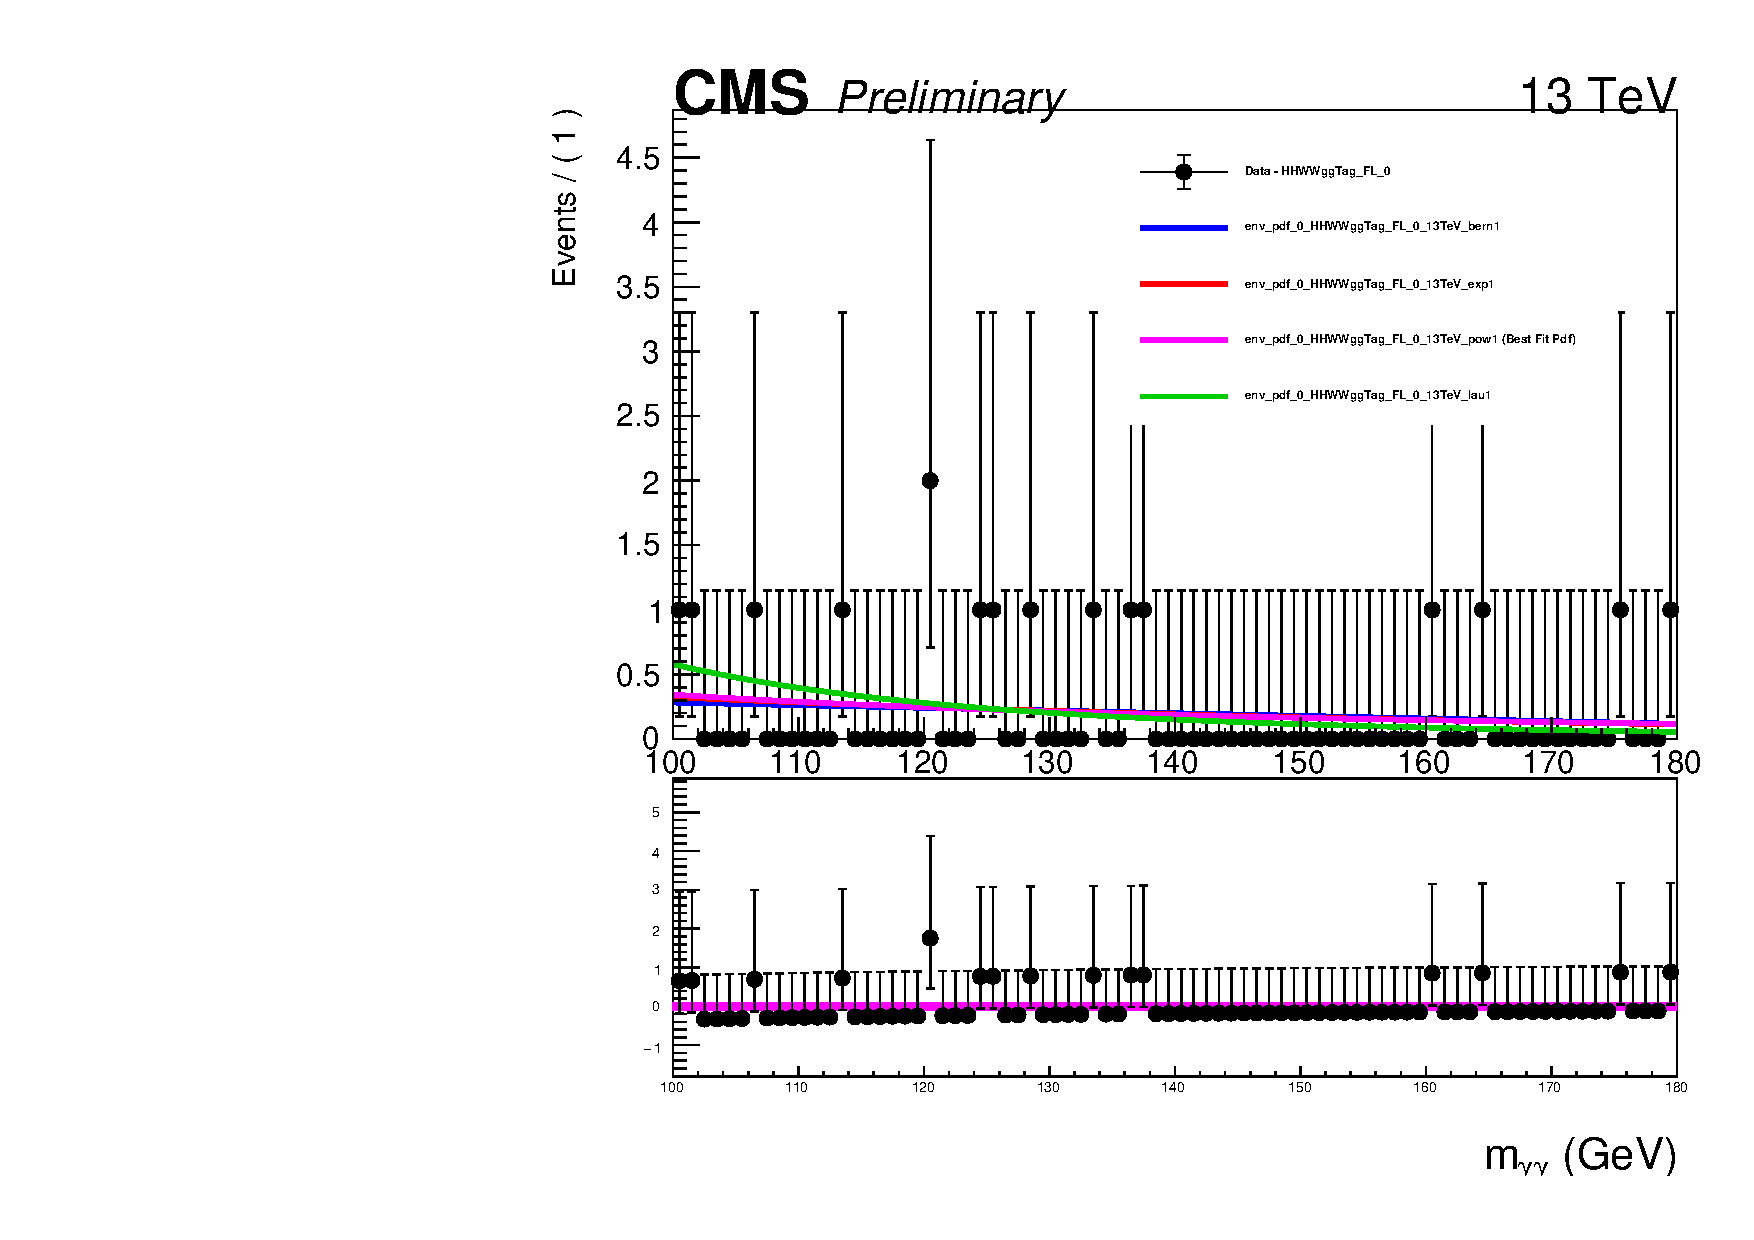
\includegraphics[width=0.45\textwidth]{Sections/HHWWgg/images/AnalyticFitting/ContinuumBackground/multipdf_HHWWggTag_FL_0_Run2.pdf}}
    \qquad
    \subfloat[Fit with uncertainty]{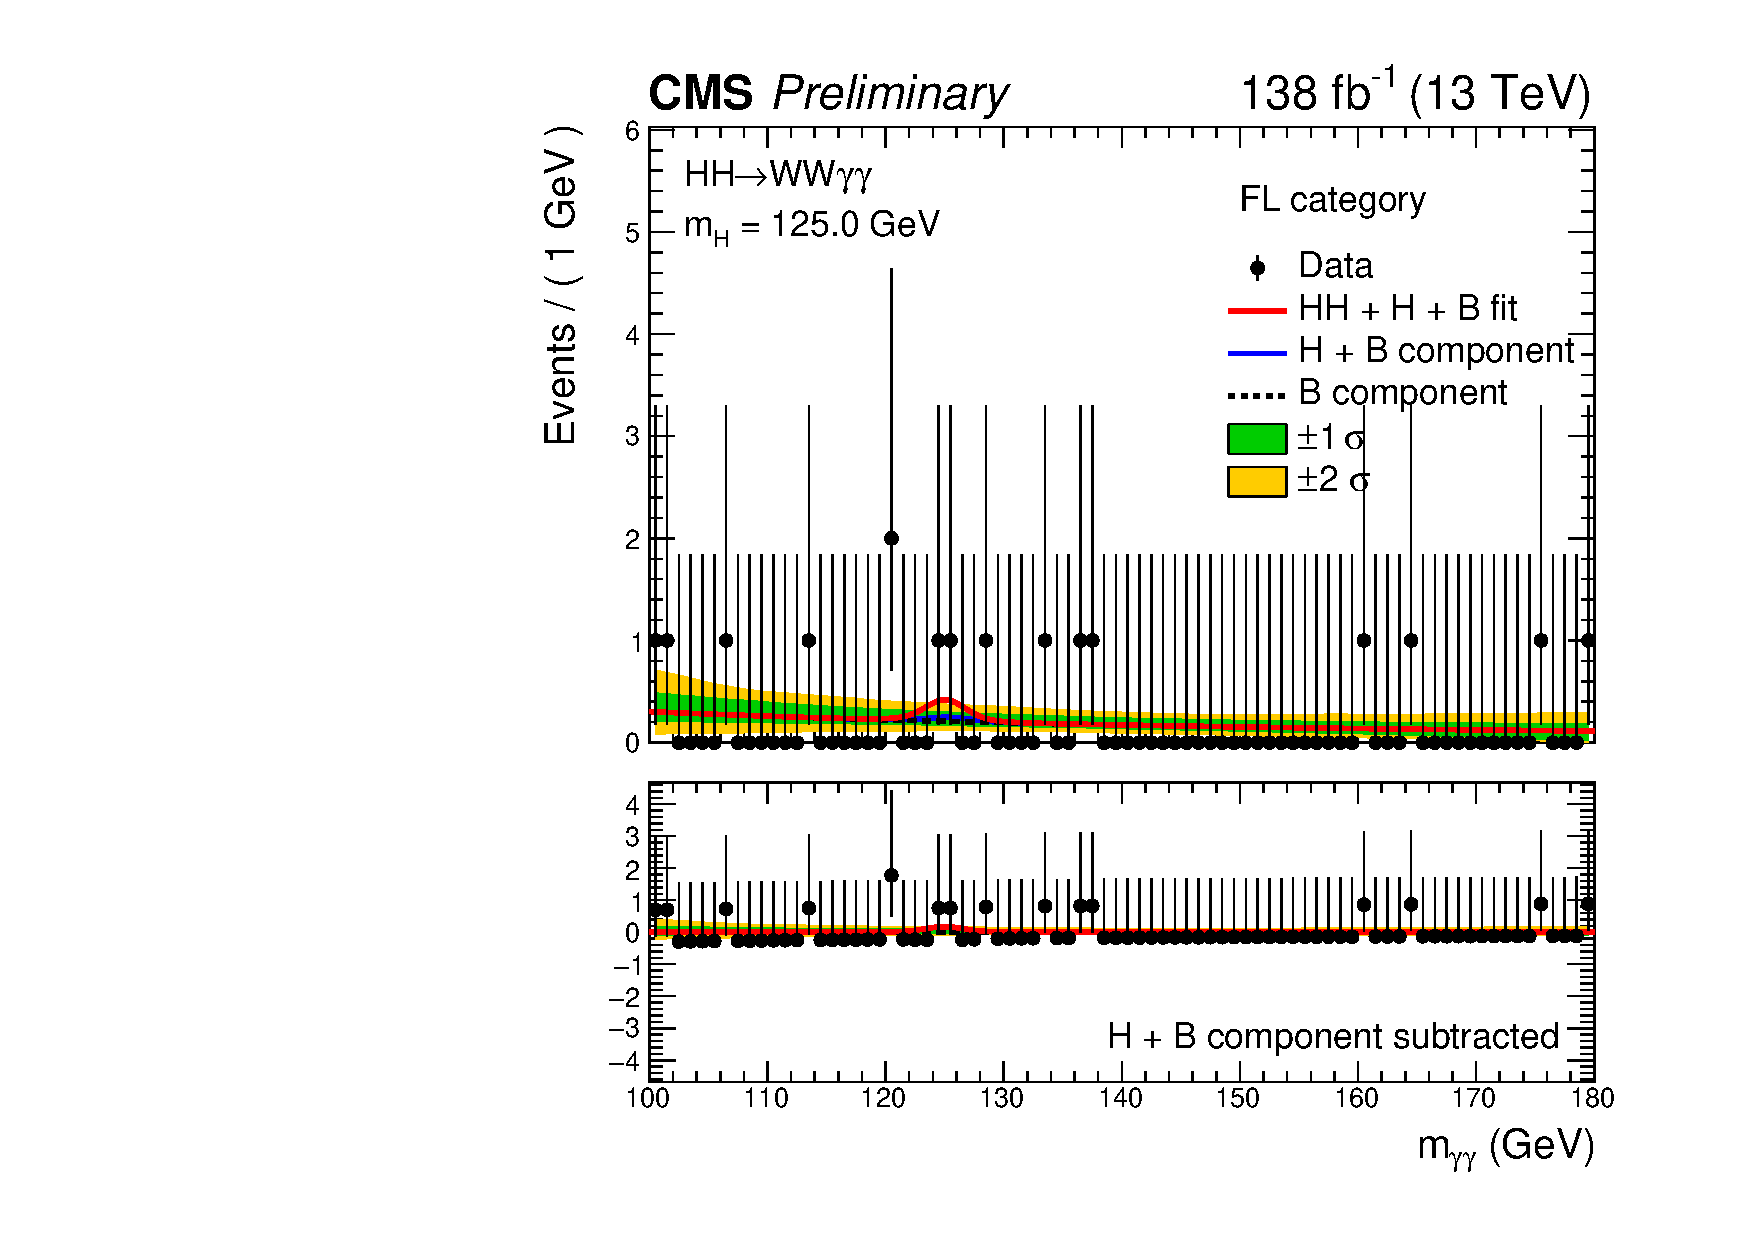
\includegraphics[width=0.45\textwidth]{Sections/HHWWgg/images/AnalyticFitting/SplusB/FL_SplusB.pdf}}
    \caption{Fully-Leptonic data-driven background model for Run 2 data}
    \label{fig:FL_DataDrivenbkg_Run2}
\end{figure}

The resulting combined fit of the background $+$ signal models to the data, where the signal strength of the HH models are varied to best fit the data, are shown in Figure \ref{fig:CombinedSPlusB} where each analysis category's contribution is weighted by its signal to background yield ratio.

\begin{figure}[!htbp]
    \centering
    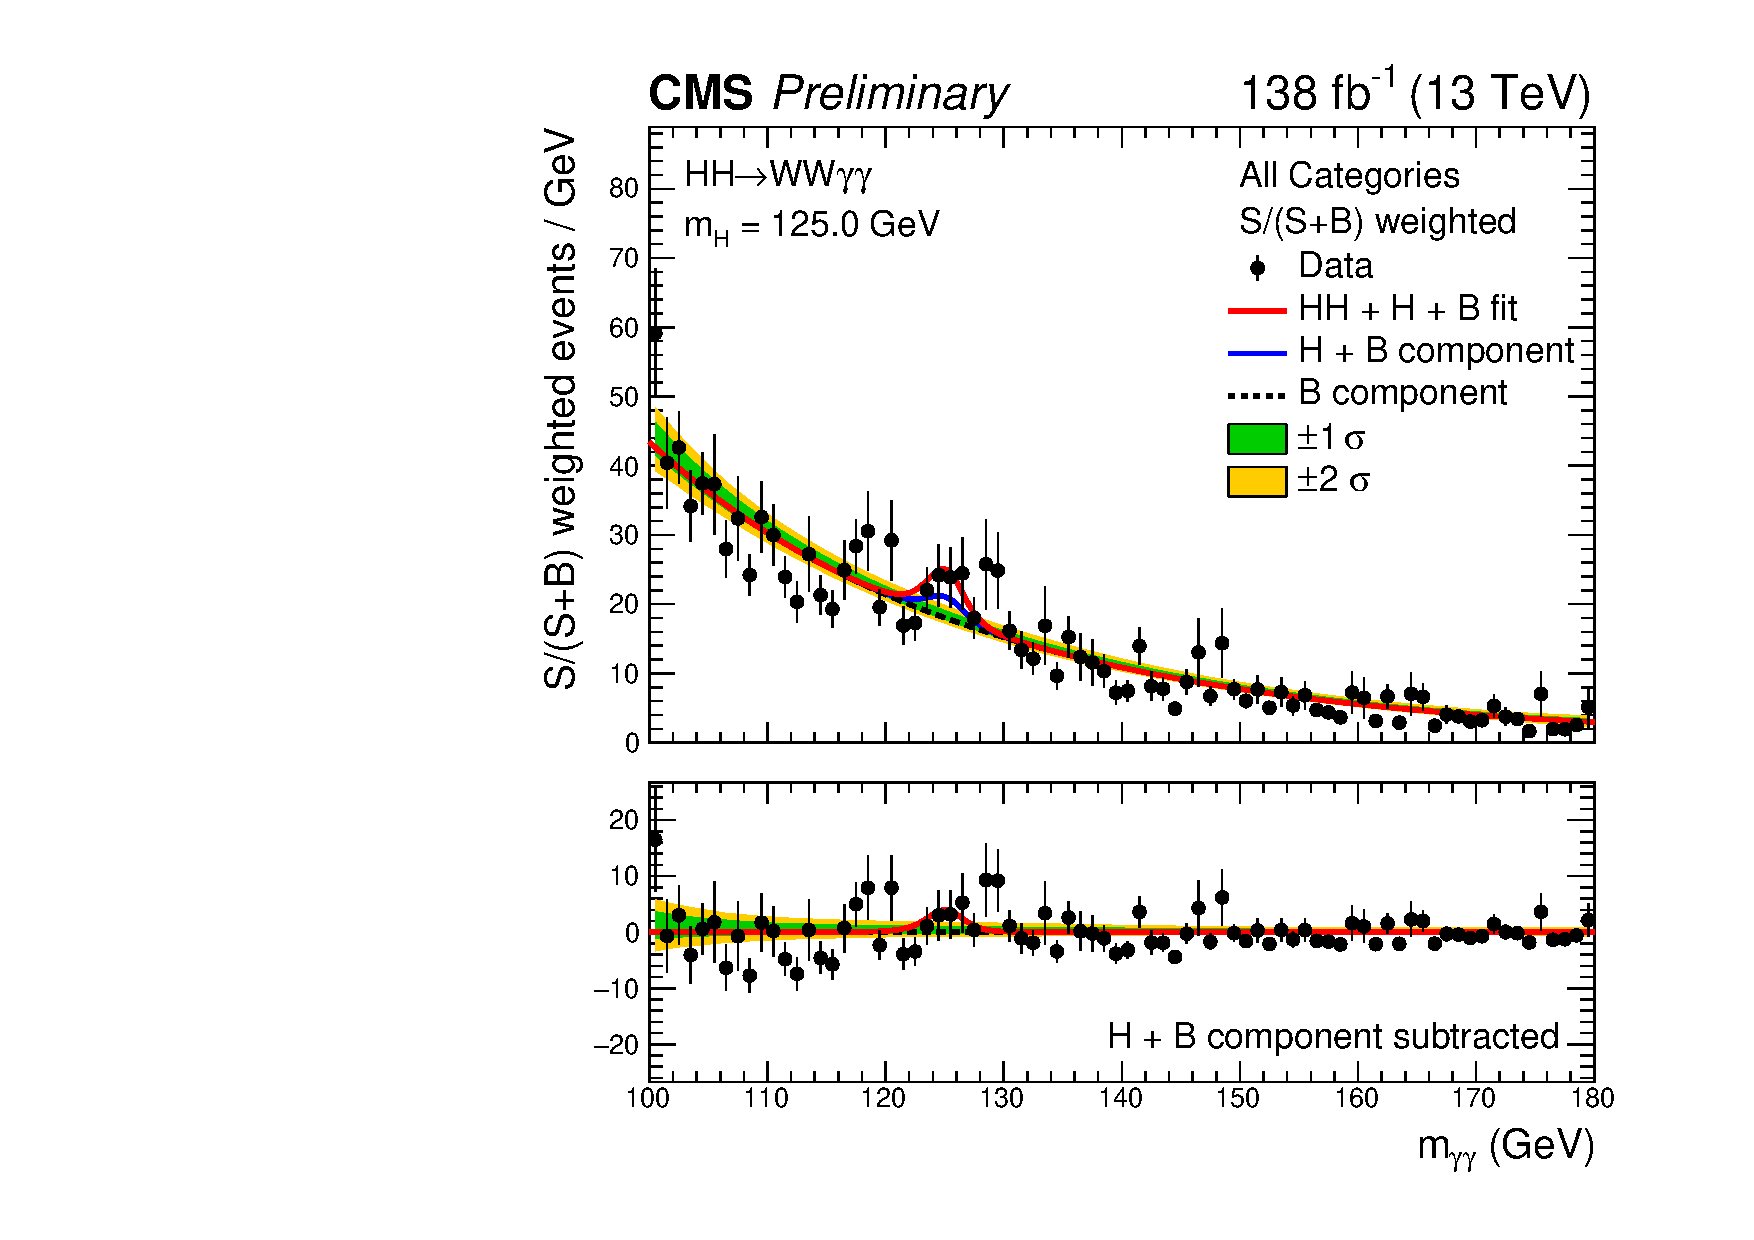
\includegraphics[width=\textwidth]{Sections/HHWWgg/images/Results/All_combined_SplusB.pdf}
    \caption{Combined signal $+$ background model fit to Run 2 data, weighted per category by S / S$+$B \label{fig:CombinedSPlusB}}
\end{figure}